 \documentclass[letterpaper,12pt]{book}
\usepackage[spanish]{babel}
\decimalpoint 
\usepackage[utf8]{inputenc}
%\usepackage{ifpdf}            %provee un switcheado facil para pdf o dvi
%\usepackage[numbers]{natbib}  %para la bibliografia
\usepackage{cite}
%\usepackage{gnuplottex} %por si se quisiera usar gnuplot directamente



\usepackage{lscape} 
\usepackage{epsfig}
\usepackage{graphics}
\usepackage{graphicx}
\graphicspath{ {figures/chapter_1/}{figures/chapter_2/} }
\usepackage{amsfonts}  
\usepackage{multicol}
\usepackage{wrapfig}   
%\usepackage[lofdepth,lotdepth]{subfig}%subs clasificados en lof y lot
%\usepackage{subfig}%subs clasificados en lof y lot
\usepackage{textcomp} 
\usepackage{subfloat} 
\usepackage{float}
%\usepackage{placeins}% provides \FloatBarrier, it prevents floats from being moved over it. 
\usepackage{multirow}
\usepackage{amsmath}
\usepackage[makeroom]{cancel}
\usepackage{amssymb} 
\usepackage{bm}
\usepackage{color} %Para poner letras con color
\usepackage{soul} %Subrayar.
\usepackage[normalem]{ulem}
\usepackage[usenames,dvipsnames]{xcolor} %Definir nombres de colores
\usepackage{url} %Para escribir urls
\usepackage{listings} %Para transcribir código
\usepackage{footnote} %Para poner footnotes en floats
\usepackage{array}
\usepackage{mathrsfs} %Font cursivo
\usepackage{enumerate}
\usepackage[T1]{fontenc}
\usepackage{booktabs}

%\usepackage{tocloft}

\usepackage[lined,boxed,commentsnumbered, algochapter]{algorithm2e}
%\usepackage{setspace}%Reducir el espacio en la biblio
%\renewcommand{\bibfont}{\small}%Letra pequeña en la biblio


%\usepackage{enumitem}%reducir espacio de items
%\setlist[1]{itemsep=-3pt}
 
% \usepackage{cleveref}
% %\crefname{section}{§}{§§}
% \crefname{section}{§}{§§}
% \Crefname{section}{§}{§§} 

%\usepackage{framed} %%%Not using it.    

%\usepackage{cite} %%%Not working

\usepackage{titlesec}         %para titulos fancy de capitulos
\usepackage{caption}  
\captionsetup[figure]{margin=0.5cm,font=small,labelfont=bf}
\captionsetup[table]{margin=0.5cm,font=footnotesize,labelfont=bf}
\captionsetup[lstlistlisting]{margin=0.5cm,font=footnotesize,labelfont=bf}
\captionsetup[algorithmcf]{margin=0.5cm,font=footnotesize,labelfont=bf}


\usepackage[list=true]{subcaption}
\captionsetup[subfigure]{margin=0.5cm,font=footnotesize,labelfont=bf}
\captionsetup[subtable]{margin=0.5cm,font=footnotesize,labelfont=bf}


%\usepackage{psfrag}             %para que texto en la figura sea remplazado
                                %incluso formulas
\usepackage[inner=3.2cm,outer=2.5cm, top=4.5cm, bottom=2.0cm]{geometry}
\usepackage[final]{pdfpages}    %para que meta facilmente paginas de pdf's

\usepackage{booktabs} %Fancy toprule, midrule, bottomrule
\usepackage{tabularx}           %tablas con anchos establecidos
\usepackage{makeidx}    %para que haga un indice de palabras. Notar:

%\usepackage{nextpage}\pagestyle{headings}
\usepackage{fancyhdr}           %para las lineas de los headers
\pagestyle{fancy}               %idem
\setlength\voffset{-0.7in}
\fancyheadoffset[LE,RO]{15pt}
%\setlength\headsep{25pt}


% Dutch style of paragraph formatting, i.e. no indents. 
\setlength{\parskip}{1.3ex plus 0.2ex minus 0.2ex}
\setlength{\parindent}{0pt}

% %******************************************************
%Mis librerías Blas

%theorem & proof packages
\newtheorem{theorem}{Theorem}[section]
\newtheorem{teorema}[theorem]{Teorema}
\newtheorem{proposicion}[theorem]{Proposición}
\newtheorem{definicion}[theorem]{Definición}
\newtheorem{corolario}[theorem]{Corolario} 
\newenvironment{proof}[1][Dem]{\begin{trivlist} %proof
\item[\hskip \labelsep {\bfseries #1}]}{\end{trivlist}}
\newcommand{\qed}{\nobreak \ifvmode \relax \else %qed
      \ifdim\lastskip<1.5em \hskip-\lastskip
      \hskip1.5em plus0em minus0.5em \fi \nobreak
      \vrule height0.75em width0.5em depth0.25em\fi}

% %******************************************************

% %* Número de cuenta
% \newcommand{\alumnocta}[1]{\def\elalumnocta{#1}}
% %* Jefe(a) de la División de Estudios Profesionales
% \newcommand{\jefeDEP}[1]{\def\eljefeDEP{#1}} 
% %* Nombre de la carrera               
% \newcommand{\nomcarrera}[1]{\def\elnomcarrera{#1}}
% %* Sinodal propietario A
% \newcommand{\sinoda}[1]{\def\elsinoda{#1}}
% %* Sinodal suplente A
% \newcommand{\suplea}[1]{\def\elsuplea{#1}}
% %* Sinodal propietario B
% \newcommand{\sinodb}[1]{\def\elsinodb{#1}}
% %* Sinodal suplente B  
% \newcommand{\supleb}[1]{\def\elsupleb{#1}}
% %* Jefe(a) del Consejo Departamental de la carrera
% \newcommand{\jefeCD}[1]{\def\eljefeCD{#1}}


% \alumnocta{40802391-7***}
% \jefeDEP{El Jefe(a) de la División de Estudios Profesionales}  %--'
% \nomcarrera{Física}
% \sinoda{El Sinodal A}
% \suplea{El Suplente A}
% \sinodb{El Sinodal B}
% \supleb{El Suplente B}
% \jefeCD{El Jefe(a) del Consejo Departamental de \elnomcarrera}

\newcommand{\titulo}{Working title on portada}
\newcommand{\titulito}{Working title on headers}
\newcommand{\nombre}{{\Large \textbf{\textsc{Blas Kolic}}}}
\newcommand{\carrera}{{\large \textsc{Físico}}}
\newcommand{\director}{{\large\textsc{Dr. Fancy Pants}}}
\newcommand{\fecha}{2017} 

%%%%%%%%%%%%%%%%%%%%%%%%%%%%%%%%%%%%%%%%%%%%%%%%%%%%%%%
%% Para asegurar que no ponga encabezados en las páginas blancas al
%% final de los capítulos que terminan en página impar.

\makeatletter
\def\cleardoublepage{\clearpage
\if@twoside
  \ifodd\c@page\else
    \hbox{}
    \thispagestyle{plain} %cambiar a empty para que no ponga el numero de pag.
    \newpage
    \if@twocolumn\hbox{}\newpage\fi
  \fi
\fi}
\makeatletter

%%%%%%%%%%%%%%%%%%%%%%%%%%%%%%%%%%%%%%%%%%%%%%%%%%%%%%%%%
%%Algunos otros detalles de fancyheaders, como pie de pagina en el exterior,
%%y que en paginas impares el titulo del capitulo se muestre a la derecha
%%y en italicas (Definicion del estilo de pagina)
\pagestyle{fancy}
\fancyhf{}
\renewcommand{\chaptermark}[1]{\markboth{ \emph{#1}}{}}
\fancyhead[LO]{}
\fancyhead[RE]{\leftmark}
\fancyfoot[LE,RO]{\thepage}


%%%%%%para activar, poner despues de \begin(document)%%%%%%%%%%%%%

%%%%%%%%%%%%%%%%%%%%%%%%%%%%%%%%%%%%%%%%%%%%%%%%%%%%%%%%%%%%%%%%

\makeindex              %hay que correr makeindex archivo.idx y luego compilar

\setlength{\headheight}{16pt} %para que no se queje por fancyheaders
\setlength{\marginparwidth}{1.5cm} %para que todonotes sea util en este caso
\definecolor{dark-red}{rgb}{0.4,0.15,0.15}
\definecolor{dark-blue}{rgb}{0.15,0.15,0.4}
\definecolor{medium-blue}{rgb}{0,0,0.5}
\definecolor{dark-green}{RGB}{50,71,13}

\ifpdf
\usepackage[pdfauthor={Kolic Blas},%
pdftitle={\titulito},%
pdftex]{hyperref} %este TIENE que ser el ultimo comando aqui
\hypersetup{   %para que aparezcan o no los cuadros de los links
  linktocpage,%make page number, not text, be link 
  colorlinks,%
  citecolor=dark-blue,%
  filecolor=black,%
  linkcolor=dark-green,%
  urlcolor=NavyBlue
  % menucolor
  % runcolor
  % anchorcolor
}
\else
  \usepackage[dvipdfm]{hyperref}
  \hypersetup{   %para que aparezcan o no los cuadros de los links
    colorlinks,%
    citecolor=dark-blue,%
  %    citecolor=black,%
    filecolor=black,%
    linkcolor=dark-red,%
  %    linkcolor=black,%
    urlcolor=black
  }
\fi

%\renewcommand{\sectionautorefname}{\S}
\def\sectionautorefname{\S$\!$}
\def\subsectionautorefname{\S$\!$}
\def\subsubsectionautorefname{\S$\!$}


\begin{document}

%%%%%%%%%%%%%%%%% DEFINICION DE COMANDOS %%%%%%%%%%%%%%%%%

\newcommand{\polk}[1]{\sum_{k=0}^n #1 x^k}
\newcommand{\polj}[1]{(\sum_{j=0}^k #1 )}
\newcommand{\pk}{{^{n}P_{\mathbb{K}}}}
\newcommand{\pkn}[1]{{^{n}P_{\mathbb{C}}^ #1 }}
\newcommand{\pkk}[2]{{^{#1}P_{\mathbb{R}}^ #2 }}
\newcommand{\algpol}{\mathcal{A}(^{n}P_{\mathbb{K}},+,\cdot)}
\newcommand{\ball}[1]{B_{#1,\bm{x}_0}(\bm{\mu})}
\newcommand{\norm}[1]{\left\lVert#1\right\rVert}
\newcommand{\afc}[1]{\hat{\Psi}^{\dagger}_#1}
\newcommand{\afa}[1]{\hat{\Psi}_{#1}}
\newcommand{\anni}[1]{\hat{a}_{#1}}
\newcommand{\crea}[1]{\hat{a}_{#1}^{\dagger}}
\newcommand{\interact}[4]{\afc{#1}\afc{#2}\afa{#3}\afa{#4}}
\newcommand{\interactt}[4]{\crea{#1}\crea{#2}\anni{#3}\anni{#4}}
\newcommand{\bra}[1]{\left\langle #1\right|}
\newcommand{\ket}[1]{\left|#1\right\rangle}
\newcommand{\tens}{\mathbin{\mathop{\otimes}}}
\newcommand{\pder}[2]{\frac{\partial #1}{\partial #2}}
\newcommand{\flowci}{\phi(t;t_0,\mathbf{x}_0)}
\newcommand{\flowU}{\phi(t;t_0,\Uxo )}
\newcommand{\flowxi}{\phi(t;t_0,\xo + \xi)}
\newcommand{\xo}{\mathbf{x}_0}
\newcommand{\xt}{\mathbf{x}(t)}
\newcommand{\dotx}{\dot{\mathbf{x}}}
\newcommand{\U}{\mathcal{U}}
\newcommand{\Uxo}{\mathcal{U}_{\xo}}
%\newcommand{\norm}[1]{\left\lVert#1\right\rVert}
%\newcommand{\pder}[3]{\frac{\partial^#3 #1}{\partial #2^#3}}

\newcommand{\ketB}[1]{\big|#1\big\rangle}
\newcommand{\braket}[2]{\left\langle #1\middle|#2\right\rangle} 
\newcommand{\braketB}[2]{\big\langle #1 \big|#2\big\rangle} 
\newcommand{\nubar}{\bar{\nu}}
\newcommand{\nutau}{\nu_{\tau}}
\newcommand{\numu}{\nu_{\mu}}
\newcommand{\nue}{\nu_e}
\newcommand{\numubar}{\bar{\nu}_{\mu}}
\newcommand{\nuebar}{\bar{\nu}_e}
\newcommand{\dmtwo}{\Delta m^2}
\newcommand{\stt}{\sin^2{ 2 \theta}}
\newcommand{\numunue}{\numu \rightarrow \nue}
\newcommand{\numunuebar}{\numubar \rightarrow \nuebar}
\newcommand{\pspace}{\left(\sin^2{ 2 \theta}, \Delta m^2\right()}
\newcommand{\pplane}{\sin^2{ 2 \theta}\mbox{--}\Delta m^2}
\newcommand{\bs}[1]{\boldsymbol{#1}}
\newcommand{\data}{\boldsymbol{D}}
\newcommand{\bgr}{\boldsymbol{B}}
\newcommand{\signal}{\boldsymbol{S}}
\newcommand{\pred}{\boldsymbol{Q}}
\newcommand{\enuqe}{E_{\nu}^{QE}}
\newcommand{\like}{\mathscr{L}}
%\newcommand{\true}{\Delta \mathscr{L_{\mathbf{V}}}}
\newcommand{\true}{\Delta \mathscr{L}}
\newcommand{\fake}{\Delta \like_{\mathbf{f}\ i}^{\{\bs{p}_0\}}}
\newcommand{\eff}{\chi^2_{\mathbf{Ef}}}%no me gusta esta notacion!!!!
\newcommand{\NF}{n_{\mathbf{f}}}
\newcommand{\critic}{\Delta\like^{\{\bs{p}_0\}}_c}


\newcommand\scalemath[2]{\scalebox{#1}{\mbox{\ensuremath{\displaystyle #2}}}}





%%%float parameters
\renewcommand{\topfraction}{0.85}
\renewcommand{\textfraction}{0.1}
\renewcommand{\floatpagefraction}{0.75}
% %%%Puse esto para los float se queden hasta arriba cuando les toca


% \makeatletter
% \setlength{\@fptop}{0pt}
% \makeatother


%\renewcommand{\contentsname}{Contenido}
\renewcommand{\bibname}{Bibliografía}
\renewcommand{\indexname}{Índice}
\renewcommand{\figurename}{Figura}
\renewcommand{\tablename}{Tabla}
\renewcommand{\listtablename}{Índice de tablas}
\renewcommand{\chaptername}{Capítulo}
\renewcommand{\appendixname}{Apéndice}
\renewcommand\lstlistingname{Código}
\renewcommand\lstlistlistingname{Código}
\renewcommand{\algorithmcfname}{Algoritmo}
\renewcommand{\listalgorithmcfname}{Índice de algoritmos y código}
%\renewcommand{\algorithmautorefname}{algoritmo}

\setcounter{tocdepth}{2}%Para que salga hasta 3=subsubsection,
                        %4=paragraph, en el índice general. 

\makeatletter
\providecommand\phantomsection{}% for hyperref

\newcommand\listofillustrations{%
    \chapter*{Índices de figuras, tablas, algoritmos y código}%
    \phantomsection
    \addcontentsline{toc}{chapter}{Índices de figuras, tablas,
      algoritmos y código}%
    \section*{Figuras}%
    \phantomsection
    \addcontentsline{toc}{section}{\protect\numberline{}Figuras}%
    \@starttoc{lof}%
    \bigskip
    \section*{Tablas}%
    \phantomsection
    \addcontentsline{toc}{section}{\protect\numberline{}Tablas}%
    \@starttoc{lot}
    \section*{Algoritmos y código}%
    \phantomsection
    \addcontentsline{toc}{section}{\protect\numberline{}Algoritmos y código}%
    \@starttoc{loa}%
    \bigskip
}
\makeatother

%\hyphenation{pa-la-bra}         %para que separe correctamente palabra
% usar \- entre silabas y en el mismo texto para evitar probs. con acentos

%%%Comandos para cambiar los identificadores en itemize
%\renewcommand{\labelitemi}{$\bullet$}
%\renewcommand{\labelitemii}{$\cdot$}
%\renewcommand{\labelitemiii}{$\diamond$}
%\renewcommand{\labelitemiv}{$\ast$}
%%%

%%% Posiblemente util para hacer una especie de itemize
%\begin{description}
%\item[Biology] Study of life.
%\item[Physics] Science of matter and its motion.
%\item[Psychology] Scientific study of mental processes and behaviour.
%\end{description}
%%%

% \tiny
% \scriptsize
% \footnotesize
% \small 	
% \normalsize
% \large 	
% \Large 	
% \LARGE 	
% \huge 	
% \Huge



%%%%%%%% Modifica formato de los titulos de los capitulos %%%%%%%

\titleformat{\chapter}[display] % cambiamos el formato de los capítulos
{\bfseries\Huge} % por defecto se usarán caracteres de tamaño \Huge en negrita
{% contenido de la etiqueta
\titlerule[2pt] % línea horizontal
\vspace{1pt}
\filleft % texto alineado a la derecha
\Large\chaptertitlename\ % "Capítulo" o "Apéndice" en tamaño \Large en lugar de \Huge
\Large\thechapter} % número de capítulo en tamaño \Large
{0mm} % espacio mínimo entre etiqueta y cuerpo
{\filleft} % texto del cuerpo alineado a la derecha
[\vspace{1pt} \noindent\rule{\textwidth}{2pt}]%\bigrule] % después del cuerpo, dejar espacio vertical y trazar línea horizontal gruesa

%%%%%%%%%%%%%%%%%%%%%%%%%%%%%%%%%%%%%%%%%%%%%%%%%%%%%%%%%%%%%%%%%%

%%%%%%%%%%%%%%%%% segunda opcion %%%%%%%%%%%%%%%%%%%%%%%%%%%%%%%%%

% \renewcommand{\thechapter}{\Roman{chapter}}
% \titleformat{\chapter}[display]
%   {\bfseries\Large}
%   {\filleft\MakeUppercase{\chaptertitlename} \Huge\thechapter}
%   {4ex}
%   {\titlerule
%    \vspace{2ex}%
%    \filright}
%   [\vspace{2ex}%
%    \titlerule]
%%%%%%%%%%%%%%%%%%%%%%%%%%%%%%%%%%%%%%%%%%%%%%%%%%%%%%%%%%%%%%%%%%%



\frontmatter %ahorraria lo de cleardoublepage hasta chaptermark. Con
             %\frontmatter se da estilo a la parte frontal del
             %libro. Todo lo que quede contenido entre \frontmatter y
             %\mainmatter, tendra un estilo en el que la numeracion de
             %pagina es con numeros romanos, y ningun capitulo, ni
             %ningun otro titulo de nivel inferior sera numerado.


%********************************
%\includepdf[pages=1]{main.pdf} %para incluir como pdf la portada
%(parece que se modifica ligeramente)
%\phantomsection
\input{Chapters/portada}
%\addcontentsline{toc}{chapter}{Portada}    
%\fullpage{1}{logoUNAM}

%\setcounter{page}{3}
%\pagenumbering{roman} %esto no sera necesario porque estamos usando frontmatter



% \newpage
% \input{Chapters/dedicatoria}        
 
\chapter{Agradecimientos} 
\documentclass[letterpaper,12pt]{book}
\usepackage[spanish]{babel}
\decimalpoint 
\usepackage[utf8]{inputenc}

\usepackage{mathrsfs}
\usepackage{amsmath}
\usepackage{amssymb}
\usepackage{amsfonts}

\begin{document}



\end{document}

% para que no haya salto de linea en el archivo toc, y por tanto no haya
% problemas en el indice
\setlength{\parskip}{0ex plus 0.5ex minus 0.2ex}
 

\pagestyle{fancy}
\fancyhead[LO]{}
\fancyhead[RE]{\emph{Índice general}}
\renewcommand{\headrulewidth}{0.5pt}

\phantomsection
\tableofcontents
\addcontentsline{toc}{chapter}{Índice general}    
\clearpage

\pagestyle{fancy}
\fancyhead[LO]{}
\fancyhead[RE]{\emph{Índices de figuras, tablas, algoritmos y código}}
\renewcommand{\headrulewidth}{0.5pt}

 \listofillustrations

 % % \setcounter{page}{1}



\newpage
\pagestyle{fancy}
\fancyhead[LO]{}
\fancyhead[RE]{\emph{Resumen / Abstract}}
\renewcommand{\headrulewidth}{0.5pt}
\addcontentsline{toc}{chapter}{Resumen / Abstract}
En esta tesis se desarrolla el concepto del transporte de jets motivado por los estudios de Daniel Pérez-Palau en \cite{Perez2013, Perez2015} y se aplica en casos particulares del problema circular de tres cuerpos. El transporte de jets integra el flujo de una ecuación diferencial alrededor de una vecindad $\U$ en lugar de una única  condición inicial $\xo$. Para hacerlo, se parametriza a $\U$ con un polinomio de $k$ variables, donde $k$ es la dimensión del espacio y se aplica a cualquier método de integración numérica, que en este trabajo será el método de Taylor por cuestiones de precisión. Como el método de Taylor depende de $\mathbf{x}_n$ para obtener a $\mathbf{x}_{n+1}$, el transporte de jets dependerá de $\mathcal{U}_{\mathbf{x}_n}$ para obtener $\mathcal{U}_{\mathbf{x}_{n+1}}$ y, como $\mathcal{U}_{\mathbf{x}_n}$ es un polinomio, operar con éste requiere de la implementación de un álgebra polinomial, que estará guiada por la construcción de Haro en \cite{Haro2009}. Las soluciones para las distintas variaciones respecto a $\mathcal{U}_{\mathbf{x}_n}$ se obtienen simplemente al evaluar el polinomio en cuestión. Al tener parametrizada toda una vecindad de $\xo$, se proponen en la tesis varios indicadores y algoritmos que aprovechan dicha parametrización.

En el problema circular de tres cuerpos se aplican dichos indicadores y algoritmos desarrollados con el transporte de jets para encontrar la probabilidad de colisión entre asteroides de diferente radio en el sistema Tierra-Luna, probar, en un sentido numérico, que el integrador preserva la simplecticidad del sistema, estudiar la sensibilidad de condiciones iniciales y analizar la variación del parámetro de masa alrededor de puntos de equilibrio del espacio de configuraciones.  

Adicionalmente, se evalúa la eficiencia, la presición y los tiempos involucrados para los algoritmos desarrollados, los cuales están disponibles en \href{https://github.com/blas-ko/tesis}{https://github.com/blas-ko/tesis} y se programaron en el lenguaje Julia, haciendo uso de los paquetes \textsf{TaylorSeries} \cite{TaylorSeries} y \textsf{TaylorIntegration} \cite{TaylorIntegration}. 

\clearpage

\pagestyle{fancy}
\fancyhead[LO]{}
\fancyhead[RE]{\emph{Introducción}}
\renewcommand{\headrulewidth}{0.5pt}
\chapter{Introducción}
\label{chap:Intro}
Las leyes que gobiernan a la Física pueden ser casi siempre presentadas como un conjunto de ecuaciones diferenciales que describen un sistema. Pensemos en la ecuación de Shrödinger de la Mecánica Cuántica, las ecuaciones de Maxwell del Electromagnetismo, las ecuaciones de Newton y las de Hamilton de la Mecánica Clásica, o las leyes de la Termodinámica en su forma diferencial, por mencionar algunas. Casi siempre se han hecho modelos simplificados y aproximaciones de la teoría para resolver preguntas específicas sobre ésta. Un ejemplo es suponer que la moléculas de un gas diluido no interactúan entre sí, lo cual permite resolver analíticamente la ecuación de estado del gas ideal, que recibe el nombre de ideal ya que no existe gas alguno que cumpla tal suposición. Considero dos principales razones por las cuales se hace ésto. La primera es para entender. Si las suposiciones son simples y la cadena lógica que nos lleva a los resultados es clara, es mucho más fácil generar intuición sobre un tema y nos permite extrapolar a casos más complicados una vez que se entiende el modelo base. En el ejemplo del gas ideal uno genera intuición sobre cómo la física estadística explica las propiedades macroscópicas como la presión, el volumen o la temperatura y, una vez que se adquiere cierta experiencia al respecto, se suelen hacer suposiciones más complejas y/o realistas como el modelo de Van der Wals, que sí toma en consideración la interacción entre las moléculas de un fluido y predice la transición de fase de éste. La segunda razón, y que va de la mano con el objetivo principal de esta tesis, es que resolver ecuaciones diferenciales de manera analítica resulta difícil en general. Nadie ha podido resolver de manera analítica el sistema de ecuaciones diferenciales que describen al problema restringido de tres cuerpos, cuyo estudio lleva más de 300 años. La dificultad de dichas ecucaciones a impulsado a analizarlas sin tener que resolverlas explícitamente. Nacen herramientas como el estudio de órbitas periódicas, puntos singulares, puntos de equilibrio, análisis de estabilidad, entre otras. Éstas no solucionan al problema, pero ayudan a entender cómo funcionan ciertos aspectos dinámicos. Sin embargo, hoy tenemos métodos para encontrar dichas soluciones sin resolverlas de forma analítica con el precio de que no son exactas del todo; éstos se conocen como métodos numéricos y métodos cualitativos.

Los métodos numéricos, a los cuales les prestaremos principal atención en este trabajo, encuentran la solución aproximada\footnote{Que las soluciones sean aproximadas no quiere decir que sean malas. Existen métodos hoy en día, como el método de Taylor, que pueden ser de precisión arbitraria si así se requiere. Actualmente la limitante es la capacidad de cómputo para hacer operaciones y el tamaño finito de la partición que representa a los números en una computadora.} de una condición inicial que represente el estado de un sistema en un momento dado. En esta tesis se propone extender el concepto de condición inicial al de vecindad inicial, lo cual se conoce como ``Transporte de Jets''. Es decir, el transporte encuentra el flujo de un conjunto de condiciones vecinas a una condición $\xo$ dada bajo un sistena de ecuaciones diferenciales ordinarias. Estas ideas ya se han abordado antes en los trabajos de Daniel Pérez-Palau \cite{Daniel2015, Perez2013, Perez2015} y en los trabajos de Makino y Berz \cite{Berz1991,Berz1998}, donde han explorado aplicaciones como la probabilidad de colisión entre satélites orbitando la Tierra, la navegación de naves espaciales via filtros de Kalman o  encontrar estructuras lagrangianas en el espacio fase. El nombre Transporte de Jets viene inspirado de la evolución de los jets en la física de partículas, que siempre vienen en paquete, tal como el jet de gluones descrito por Peskins en \cite{Peskin1996}.

La tesis está organizada de la siguiente manera: El capítulo \ref{chap:jt} presenta el concepto de transporte de jets como extensión de los métodos numéricos, específicamente montándolo sobre el método de Taylor, se construye un álgebra polinomial necesaria para las operaciones de las vecindades, y finalmente se pone a prueba al transporte en una serie de ejemplos hamiltonianos sencillos. El capítulo \ref{chap:jt_indicators} desarrolla una serie de indicadores dinámicos para el transporte de jets, donde se aprovecha el carácter paramétrico de las vecindades. El capítulo \ref{chap:CR3BP} estudia al problema circular de tres cuerpos, donde se analizan sus ecuaciones, sus puntos de equilibrio, sus constantes de movimiento y la estructura del espacio de configuraciones. Finalmente, el capítulo \ref{chap:results} presenta los resultados principales utilizando los conceptos del capítulo \ref{chap:jt} y los indicadores de \ref{chap:jt_indicators} en el problema circular de tres cuerpos desarrollado en el capítulo \ref{chap:CR3BP}. 


%Párrafo inicial con un poquito de historia, que de razones para alzar el estudio de ecuaciones diferenciles, específicamente los métodos numéricos. 
%Un poco la historia de cómo surge el jet transport y la motivación de querer usarlo. Aquí se menciona el objetivo 
%Hablar de la relación del JT con el P3C y por qué es un buen caso de estudio.

% Para que de nuevo haya salto de linea. (buscar Dutch style)
\setlength{\parskip}{1.3ex plus 0.2ex minus 0.2ex}


           



\mainmatter %Estilo del texto principal del documento, en que las
            %paginas seran numeradas con numeros arabigos y los
            %capitulos y titulos de nivel inferior, si seran
            %numerados.

% Ajuste de los encabezados de nuevo para que esta vez, las paginas impares
% tengan el capitulo a la izquierda, y las pares tendran capitulo x a la
% derecha.
\fancyhead[LO]{\leftmark}
\fancyhead[RE]{\emph{Capítulo \thechapter}}

%%%%%%%%%%%%%%%%% CAPÍTULOS %%%%%%%%%%%%%%%%%

\chapter{Transporte de Jet (TJ)} 
\label{chap:jt}
Consideremos un sistema de ecuaciones diferenciales ordinarias (EDO) descrito por 
\begin{equation}
\dot{\mathbf{x}}(t) = f(\mathbf{x}(t),t)
\label{eq:ode}
\end{equation}
con $t$ el parametro que describe la evolución del sistema y $\flowci$ la trayectoria o \textbf{flujo} de la solución que en $t_0$ se encuentra en $\xo$. En la mayoría de los sistemas físicos, el parámetro $t$ describe al tiempo, i.e., $t \in \mathbb{R}^+$, y al sistema de ODE se le conoce como sistema dinámico.

Pocos son los casos en donde la solución a $\dot{\mathbf{x}}(t)$ se puede obtener de manera analítica y, por tanto, estudiar las familias de soluciones para diferentes condiciones iniciales termina siendo, casi siempre, un estudio indirecto o aproximado. Se han considerado varias formas para darle la vuelta a este problema y, en los esfuerzos de lo aproximado, una de las soluciones más prácticas ha sido discretizar al parámetro temporal $t$ de (\ref{eq:ode}) y encontrar, en saltos discretos de $t$, el ``estado actual'' del sistema dado un ``estado anterior''.

Gracias a que hoy en día existe poder de cómputo para hacer muchas operaciones simples en relativamente poco tiempo, se ha explotado el estudio y uso de métodos iterativos para obtener $\flowci$, siendo de gran utilidad en los últimos años. Éstos se conocen como \textbf{métodos numéricos de integración de ecuaciones diferenciales}. Con estos métodos se puede, en la mayoría de los casos, definir una condición inicial $\xo := \mathbf{x}(t_0)$ y obtener la solución para esta condición particular. Sin embargo, no siempre es suficiente obtener la solución de una única condición inicial dada y, muchas veces, interesa todo una familia de soluciones alrededor de un punto $\xo$ de interés. Esto puede pasar, por ejemplo, en aceleradores de partículas que disparan paquetes de onda como si fuesen ``gotas" sujetas a algún campo externo. En mecánica de fluidos es interesante estudiar parcelas de fluidos y, con la representación lagrangiana de las ecuaciones de Navier-Stokes, ver cómo evolucionan estas parcelas en el tiempo; ésta es una rama muy utilizada por los métodos computacionales, ya que por las no linealidades de las ecuaciones de Navier-Stokes, ha sido muy difícil obtener soluciones analíticas sin hacer un montón de aproximaciones previas. En sistemas de muchos cuerpos también se ha pensado en familias de soluciones cercanas, ya que difícilmente se conocen las condiciones iniciales de todo el sistema con una precisión profunda, de hecho, en todos los sistemas donde las condiciones iniciales pueden no saberse con exactitud, un método exhaustivo sería el conseguir todas las soluciones de las posibles condiciones iniciales para estos sistemas. Una rama muy relacionada a lo anterior son los métodos de Montecarlo, donde, en el caso de las EDO, se consigue una distribución inicial de condiciones iniciales y se obtiene cada una de las soluciones para éstas. 
En un plano más general, el mundo de las ecuaciones diferenciales ordinarias ha estudiado exhaustivamente los campos vectoriales que generan las ecuaciones de la forma (\ref{eq:ode}). Ha habido gran interés en entender el comportamiento de órbitas periódicas y puntos singulares o, más generalmente, la topología del campo vectorial que representa las soluciones de las ecuaciones. Se han desarrollado métodos para encontrar estructuras hiperbólicas en el espacio fase y métricas para catalogar el comportamiento de las soluciones. Algunos de los resultados teóricos para esto son el número de Euler, que categoriza la topología del espacio, las secciones de Poincaré, que son representaciones de la solución en un espacio de menor dimensionalidad, donde normalmente se busca que no sea tangente a las soluciones para entender cómo éstas cruzan dichas secciones que describe, los exponentes de Lyapunov, que estudia la separación de soluciones cercanas a una condición inicial dada, la derivada de Lie, que compara al campo vectorial de (\ref{eq:ode}) contra otro campo vectorial, la linealización de Grobman-Hartman, que toma la parte lineal de $\dot{\mathbf{x}}(t)$ en localidades suficientemente pequeñas y analiza qué quiere decir ``suficientemente'', entre otras. 
%%REFERENCIAS NECESARIAS EN EL PÄRRAFO ANTERIOR.

Muchas de estas preguntas podrían responderse si en vez de encontrar $\flowci$ para una condición $\mathbf{x}_0$ dada se tuviera una vecindad inicial $\U$ alrededor de $\mathbf{x}_0$ (que llamaremos $\Uxo$) y se encuentra el flujo para toda esta parcela. Ésto viene motivado principalmente por los trabajos de Daniel-Perez sobre aplicaciones del TJ, \cite{Perez2013,Perez2015}. Parecería una idea idéntica a las simulaciones de Montecarlo, pero la gran diferencia es que en Montecarlo se integra cada solución de manera independiente y aquí se integra toda la vecindad $\Uxo$ a la vez. Ésta es la principal motivación detrás del Transporte de Jets (TJ); dada la vecindad inicial $\U_{\xo}$ alrededor de $\xo$ parametrizada por el vector $\mathbf{\xi}$, se busca obtener $\flowxi$ y evaluar $\xi$ en $\Uxo$ para obtener $\flowU$, la deformación de la vecindad $\U_{\xo}$ al tiempo $t$. La idea operativa computacional del TJ es muy similar a la de cualquier método numérico de integación de EDO: discretiza los pasos del parámetro de evolución (tiempo) en intervalos $h_n$ y encuentra un método iterativo para conseguir el siguiente punto del flujo $\flowci$. En la figura \ref{fig:FIGURA!} se observa un esquema cualitativo de la idea del transporte de jets.

%FIGURA!

Merece la pena ilustrar dicha discretización con un método muy sencillo e intuitivo aunque, al  no ser tan preciso, se usará otro para el desarrollo de esta tesis.

Sabemos, por definición, que 
\begin{equation*}
 \dot{\mathbf{x}}(t) = \lim_{h\to 0} \frac{\mathbf{x}(t+h)-\mathbf{x}(t)}{h}.
\end{equation*}  

Si tomamos $h$ \textit{suficientemente pequeña}, aunque finita, podemos aproximar
\begin{equation*}
 \mathbf{x}(t+h) \approx \mathbf{x}(t) + h \dot{\mathbf{x}}(t)
\end{equation*}

que, si tomamos en cuenta que $\dot{\mathbf{x}}(t) = f(\mathbf{x}(t),t)$ y que $h$ es un paso de integración, se obtiene
 
\begin{equation}
 \mathbf{x}_{n+1} = \mathbf{x}_n + h f(\mathbf{x}_n,t_n)
 \label{eq:euler} 
\end{equation}

que se conoce como el \textbf{Método de Euler}. Así, dada $\xo$ se puede obtener $\flowci$ iterando (\ref{eq:euler}) hasta llegar a $t$ en pasos de $h$.

Ahora, para la evolución del TJ se parametriza a la vecindad $\U_{xo}$ usando un polinomio $P_{t_0,\xo}(\xi)$ alrededor de $\xo \in \mathbb{R}^n$ 
\begin{equation*}
 P_{t_0,\xo}(\xi) = P_{0,\xo}(\xi) = \xo + \xi = \xo + \left( \xi_1, \xi_2, ..., \xi_n \right)^T
\end{equation*} 

y se evalúa con el método de Euler (o cualquier otro) para obtener el flujo de $\Uxo$ en algún tiempo $t$ posterior $\flowU$
\begin{equation*}
P_{1,\xo}(\xi) := P_{t_0+h,\xo}(\xi) = P_{t_0,\xo}(\xi) + h f(P_{0,\xo},t_0) = \xo + \xi + h f(\xo + \xi).
\end{equation*}

Así, se puede extender el método de Euler al TJ 
\begin{equation}
 P_{t_n,\xo}(\xi) = P_{n,\xo}(\xi) = P_{n-1,\xo}(\xi) + h f(P_{n-1,\xo}(\xi),t_{n-1})
 \label{eq:eulerU}
\end{equation}

donde $P_{n,\xo}(\xi)$ representa al flujo $\flowxi$. Basta evaluar éste polinomio en $\Uxo$ para obtener $\flowU$\footnote{$\flowxi$ no necesariamente debe ser evaluado en toda una vecindad $\Uxo$; puede, también, ser en un único punto $\xi =\delta \mathbf{x}$ y obtener el flujo para $\phi(t;t_0,\xo + \delta \mathbf{x})$}.

Es importante notar que la solución $\flowci$ o el conjunto de soluciones $\flowU$ son sensibles al método de integración utilizado para encontrarlas dado que la solución construida es una aproximación. Se recomienda al lector, si le interesa, leer el desarrollo explícito en \cite{Perez2015} para ver estas diferencias.

Para ilustrar un poco lo anterior, merece la pena desarrollar un ejemplo que motive el uso del Transporte de Jet.

Sea
\begin{align}
\dotx = f(\mathbf{x},t) = \left[ \begin{array}{cc}
 0 & -1  \\
 1 & 0  \\
\end{array} \right] \left( x_1, x_2 \right)^T
\label{eq:center}
\end{align}
un campo vectorial que describe centros alrededor de $x_0 = (0,0)$. 

Si se toma $P_{0,\xo} = (x_{1_0},x_{2_0}) + (\xi_1,\xi_2)$ como la vecindad inicial, podemos desarrollar ``a mano'' el transporte de Jet, donde, usando el método de Euler tenemos

\begin{align*}
\mathbf{x}_1 &= P_{1,\xo}(\xi) = P_{0,\xo}(\xi) + h f(P_{0,\xo}(\xi),t_0) \\
&= (x_{1_0} - h x_{2_0}, h x_{1_0} + x_{2_0} )^T + \left[ \begin{array}{cc}
 1 & -h  \\
h & 1  \\
\end{array} \right] (\xi_1,\xi_2)^T.
\end{align*} 

El primer término de $\mathbf{x}_1$ corresponde al primer paso de integración de $\xo$ sin el transporte de jets. El segundo término es la solución de las ecuaciones variacionales de primer order para el primer paso con el método de Euler, o dicho de otra manera, una aproximación lineal de soluciones cercanas a $\xo$ parametrizadas por las $\xi$'s. Gracias a esta parametrización, es natural pensar en obtener soluciones cercanas simplemente evaluando $\xi$ en $P_{1,\xo}(\xi)$ o, más generalmente, en $P_{n,\xo}(\xi)$. De este modo, el TJ se plantea a ser un buen método para hacer simulaciones de Montecarlo de manera muy rápida, ya que habría que hacer una sola integración de $\U_{\xo}$ y después simplemente evaluar los polinomios. La única desventaja en esto es que la integración de $\U_{\xo}$, al operar siempre con polinomios y no con números, suele ser más lenta que la de una única trayectoria que pasa por $\xo$ en $t_0$. Naturalmente, el tiempo en donde uno u otro método es mejor es discutible y dependerá fuertemente de la complejidad y la dimensionalidad de las ecuaciones presentes en el sistema\footnote{Para una discusión más a fondo sobre este tema, revisar la sección \ref{sec:}, donde se hacen varios benchmarks en relación al tiempo de cómputo y la memoria utilizada.}.

Se podría seguir haciendo el desarrollo del TJ iterativamente con el método de Euler. Por ejemplo, el segundo paso quedaría como 
\begin{align*}
\mathbf{x}_2 =& P_{2,\xo}(\xi) = P_{1,\xo}(\xi) + h f(P_{1,\xo}(\xi),t_n) \\
=& (x_{1_0} - h x_{2_0}, h x_{1_0} + x_{2_0} )^T + \left[ \begin{array}{cc}
 1 & -h  \\
h & 1  \\
\end{array} \right] (\xi_1,\xi_2)^T \\ 
&+ h \left( \left[ \begin{array}{cc}
 0 & -1  \\
 1 &  0  \\
\end{array} \right] \left( (x_{1_0} - h x_{2_0}, h x_{1_0} + x_{2_0} )^T + \left[ \begin{array}{cc}
 1 & -h  \\
h & 1  \\
\end{array} \right] (\xi_1,\xi_2)^T \right) \right) \\
=& \left[ \begin{array}{c}
x_{1_0} - h^2x_{1_0} - 2h x_{2_0}  \\
2h x_{1_0} + x_{2_0}  - h^2x_{2_0}  \\
\end{array} \right] + \left[ \begin{array}{cc}
 1-h^2 & -2h  \\
2h & 1-h^2  \\
\end{array} \right] (\xi_1,\xi_2)^T
\end{align*}
 
y así sucesivamente. Una vez que se obtiene $P_{n,\xo}(\xi)$ basta con evaluarlo para valores $\mathbb{\xi}$ \textit{suficientemente pequeños} para encontrar las soluciones en la vecindad de $\xo$. En la figura \ref{fig:center-evals} se evalúa $\flowxi$ para distintos valores de $t$ en vecindades $\Uxo$ dadas por círculos de distinto radio.

se pueden ver las evaluaciones de $P_{n,\xo}(\xi)$ para distintos valores de $t_n$ y de $\xi$ alrededor del punto singular $\xo = (0,0)$.

%FIGURA!
\begin{figure}[h!]
 \centering
 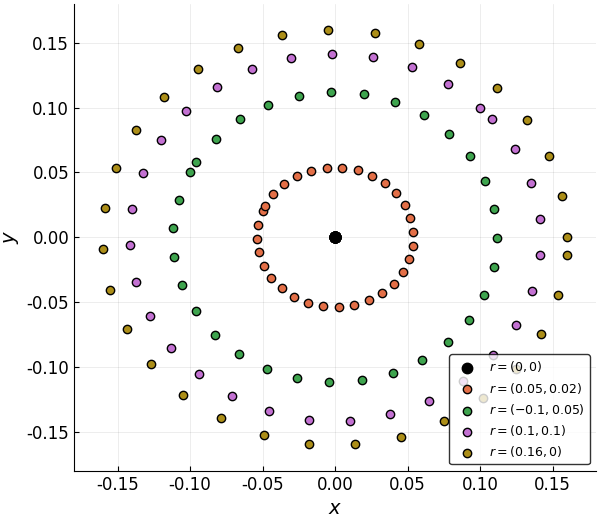
\includegraphics[width=0.8\linewidth]{euler-jt-evaluations-center}
 \caption{Transporte de jets para la ecuación (\ref{eq:center}) con condición inicial $\xo = (0,0)^T$ usando el método de Euler para $\Uxo$ parametrizada en un círculo $\xi(\tau) = r\left( \cos(\tau),\sin(\tau) \right)$ para un intervalo temporal $[0,2\pi]$ en pasos de $h=10^{-4}$. Se evaluó la solución para los distintos $r$'s marcados en la gráfica, en intervalos de $1000h$.}
 \label{fig:center-evals}
\end{figure}

Notemos que (\ref{eq:center}) corresponde a un sistema hamiltoniano cuyas soluciones en el espacio fase viven en las curvas de nivel dadas por
\begin{equation*}
H(\mathbf{x}) = \frac{1}{2} \left( x_1^2 + x_2^2 \right),
\end{equation*} 
con solución analítica
\begin{align}
 x_1(t) &= x_{01}\cos{(t)} - x_{02}\sin{(t)} \nonumber \\
 x_2(t) &= x_{01}\sin{(t)} + x_{02}\cos{(t)}.
 \label{eq:center_analytical}
\end{align}

En la figura \ref{fig:center_anal_comparison} se muestran distintas comparaciones de la integración numérica contra las soluciones analíticas de (\ref{eq:center_analytical}).

%FIGURA! 
\begin{figure}[h!]
\centering
\begin{subfigure}{0.49\textwidth}
	\centering
	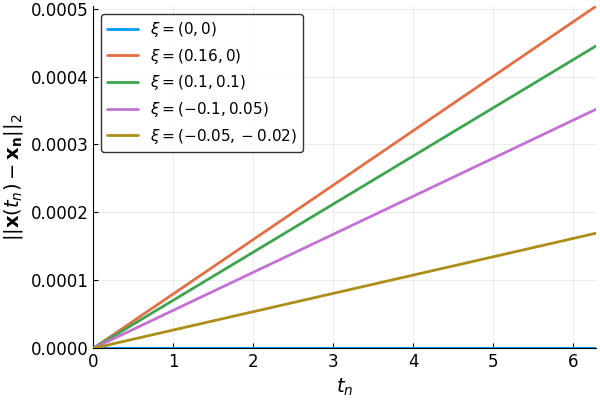
\includegraphics[width = \textwidth]{euler-vs-analytical_center}
	\caption{Norma de la diferencia entre la solución real y evaluaciones de la solución numérica para distintos valores de $\xi$ marcados en la gráfica. Se puede observar un crecimiento lineal del error numérico, lo cual es una de las consecuencias de usar el método de Euler.}
	\label{fig:center-eu_vs_anal}
\end{subfigure}
%
\begin{subfigure}{0.49\textwidth}
	\centering
	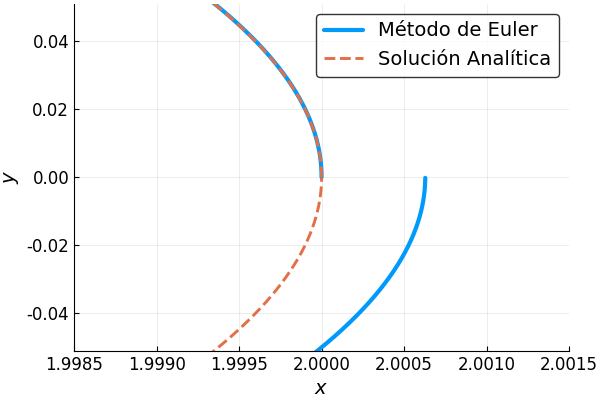
\includegraphics[width = \textwidth]{euler-method_error}
	\caption{Sección del espacio fase donde se observan la solución analítica y la solución numérica para pasos de $h=10^{-4}$ con cóndición inicial $\xo = (2,0)$. \\ \\}
	\label{fig:center_not-closed}
\end{subfigure}
\caption{Diferencias numéricas entre el método de Euler y la solución analítica para \ref{eq:center}}
\label{fig:center_anal_comparison}
\end{figure}


Queda claro que el desarrollo de TJ necesita de un álgebra polinomial para poder evaluar los distintos $P_{j,\xo}(\xi)$ que definen al campo vectorial en cada uno de sus pasos. El problema de evolucionar una vecindad $\U_{\xo}$ dado un sistema dinámico $\dot{\mathbf{x}}(t) = f(t,\mathbf{x}(t))$ se reduce al problema de saber cómo se evalúan distintos polinomios en cada paso de integración, así como la definición computacional de sus operaciones. Hay muchos detalles a considerar en este problema: ¿Qué paso de integración se deberá usar para conseguir la evolución temporal de las soluciones? ¿Cómo medimos el error respecto a la solución real? ¿Existe alguna forma de controlar el error que arrojan el método de integración y la propagación de jets del TJ? ¿Cuál es la complejidad de las operaciones para la aritmética de polinomios? En la siguiente sección \ref{sec:alg_poli} se desarrolla el álgebra polinomial y sus operaciones tal como son implementadas en el TJ y se ahonda en esta discusión. En la sección \ref{sec:taylor-metodo} se hace el desarrollo del método de Taylor como integrador computacional adaptativo de sistemas de EDO. En el siguiente capítulo se desarrollarán herramientas a partir del transporte de jets y sus características así como sencillos ejemplos ilustrativos para cada una de ellas.


\section{Álgebra Polinomial}
\label{sec:alg_poli}

La necesidad del álgebra polinomial se vuelve imperativa para el TJ como hemos visto en la sección anterior. Haremos la construcción de manera formal donde denotaremos  dicha álgebra como $\algpol$ donde $\pk$ es el conjunto de \textbf{polinomios de orden $n$ con coeficientes en el campo $\mathbb{K}$} tal que, si  $P(x) \in \pk$, éste se define como
$$P = P(x) := \polk{p_k} $$
con $P: \mathbb{C} \to \mathbb{K}$ una función analítica y $p_k \in \mathbb{K} \  \forall i \in [0,n]$.

Esta sección se divide en tres: la primera sobre construcción formal del álgebra en una variable vía la demostración de sus propiedades de campo, la segunda sobre el desarrollo de las operaciones para las funciones estándar dentro de ésta álgebra. La tercera sección es la extensión de dicha álgebra a más variables, para poder trabajar a cualquier dimensionalidad

%		- It may be necessary to analize how different independet variables imply that A(x) != A(b).

\subsection{Construcción del Álgebra}
\label{sec:alg_field}

Inspirado en la aritmética usual en $\mathbb{C}$ o $\mathbb{R}$, podemos definir $(+,\cdot)$ para $\algpol$ de la siguiente manera:

Sean $A,B \in \pk$ con $A = \polk{a_k}$ y $B = \polk{b_k} \ a_k,b_k \in \mathbb{K} \ \forall k \in [0,n]$, entonces, para la suma, notemos que
\begin{align*}
\polk{a_k} + \polk{b_k} =& a_0 + a_1 x + \cdots a_n x^n + b_0 + b_1 x + \cdots + b_n x^n \\
=& (a_0 + b_0) + (a_1 + b_1) x + \cdots + (a_n + b_n)x^n = \polk{(a_n + b_n)} 
\end{align*}
así, se define \textbf{$+$}  en $\pk$ como
\begin{equation}
A + B = \polk{(a_k + b_k)}.
\label{eq: polsum}
\end{equation}

Para el producto, notemos que
\begin{align*}
\polk{a_k}\cdot\polk{b_k} =& (a_0 + a_1 x + \cdots + a_n x^n)\cdot(b_0 + b_1 x + \cdots + b_n x^n) \\
=& (a_0b_0) + (a_1b_0 + a_0b_1) x + (a_2b_0 + a_1b_1 + a_0b_2) x^2 + \cdots + \\
+& \sum_{j=0}^n a_{n-j}b_j x^n + \mathcal{O}(x^{n+1}) = \polk{ \polj{a_{k-j}b_j } }
\end{align*}

así, se define \textbf{$\cdot$}  en $\pk$ como

\begin{equation}
A \cdot B = \polk{\sum_{j=0}^k a_{k-j}b_j}.
\label{eq: polprod}
\end{equation}
Aún cuando las operaciones están definidas inspiradas en la aritmética de los números, $\mathbb{K}$ puede ser cualquier campo arbitrario.

\begin{proposicion}
Para $\mathbb{K} = \mathbb{R}$ o $\mathbb{C}$, $\algpol$ forma un campo.
\label{prop:alg_field}
\end{proposicion}

\begin{proof}
Basta probar las nueve propiedades de campo con las operaciones de \ref{eq: polsum} y \ref{eq: polprod}.
Sean $A$, $B$ y $C \in \pk$
\begin{enumerate}

 \item $ A + B = B + A $
 \begin{proof}
  \begin{align*}
   A + B =& \polk{a_k} + \polk{b_k}  = \polk{(a_k + b_k)} \\ 
   =& \polk{(b_k + a_k)} = \polk{b_k} +     \polk{a_k} = B + A
  \end{align*}
 \end{proof}
 
 \item A + (B+C) = (A+B) + C
 \begin{proof}
  \begin{align*}
   A + (B+C) =& \polk{a} + \polk{(b_k+c_k)} = \polk{(a_k + (b_k + c_k))} \\
   =&  \polk{((a_k + b_k) + c_k)} = \polk{(a_k+b_k)} + \polk{c_k} \\
   =& (A+B) + C 
  \end{align*}
 \end{proof}
 
 \item $\exists \  \bm{0} \in \pk \text{ tal que }  \bm{0} + A = A $
 \begin{proof}
 Sea $\mathbb{0} = \bm{0}(x) = \polk{\sigma_k}$ donde $\sigma_k = 0 \ \forall k \in [0,n]$, así 
  \begin{align*}
  \bm{0} + A = \polk{(\sigma_k + a_k)} = \polk{(0 + a_k)} = \polk{a_k} = A
  \end{align*}
 \end{proof}
 
 \item $\exists \ {-A} \in\pk  \text{ tal que } A + (-A) = 0 $
 \begin{proof}
 Sea $-A = -A(x) = \polk{\mathrm{a}_k}$ donde $\mathrm{a}_k = -a_k \ \forall k \in [0,n]$, así
  \begin{align*}
   A + (-A) = \polk{(a_k + \mathrm{a}_k)} = \polk{(a_k + (-a_k))} = \polk{0} = \bm{0}
  \end{align*}
 \end{proof}
 
 \item $ A\cdot B = B\cdot A $
 \begin{proof}
 Hay que probar, básicamente, que $\sum_{j=0}^k{a_{k-j}b_j} = \sum_{j=0}^k{b_{k-j}a_j}$:
  \begin{align*} 
   \sum_{j=0}^k{a_{k-j}b_j} =& \sum_{i=0}^k{a_ib_{k-i}} \text{ con } i = k - j \\
   =& \sum_{i=0}^k{ b_{k-i}a_i } = \sum_{j=0}^k { b_{k-j}a_j }
  \end{align*}
  $\therefore A\cdot B = B\cdot A$.
 \end{proof}
 
 \item $ (A \cdot B) \cdot C = A \cdot (B \cdot C) $
 \begin{proof}
 Por un lado
  \begin{align*}
  A \cdot (B \cdot C) =& \polk{a_k}\ \polk{ \polj{b_{k-j}c_j} } = \polk{\big(  \sum_{j=0}^ka_{k-j}\sum_{i=0}^jb_{j-i}c_i \big)} \\
  =& \polk{\big(  \sum_{r+j=k}a_r\sum_{p+i=j}b_pc_i \big)} = \polk{\big(  \sum_{r+j=k}\sum_{p+i=j}a_rb_pc_i \big)} \\
  =& \polk{\big(  \sum_{r+p+i=k}a_rb_pc_i \big)} 
  \end{align*}
  por otro
    \begin{align*}
  (A \cdot B) \cdot C =& \polk{ \polj{a_{k-j}b_j} }\ \polk{c_k} = \polk{\big( \sum_{i=0}^ja_{j-i}b_i  \sum_{j=0}^kc_{k-j} \big)} \\
  =& \polk{\big(  \sum_{r+j=k}(\sum_{p+i=r}a_pb_i) c_j \big)} = \polk{\big(  \sum_{r+j=k}\sum_{p+i=r}a_pb_ic_j \big)} \\
  =& \polk{\big(  \sum_{p+i+j=k}a_pb_ic_j \big)} 
  \end{align*}
  
  Basta ver que, por un cambio de nombre de índices $p \to r$, $i \to p$, $j \to i$,
  \begin{align*}
   \sum_{p+i+j=k}a_pb_ic_j = \sum_{r+p+i=k}a_rb_pc_i
  \end{align*}   
  $\therefore (A \cdot B) \cdot C = A \cdot (B \cdot C)$.
 \end{proof}
 
 \item $\exists \ \textbf{1} \in \pk \text{ tal que } \textbf{1}\cdot A = A $
 \begin{proof}
 Sea $ \textbf{1} = \textbf{1}(x) = \polk{\omega_k}$ donde $\omega_k = 0 \ \forall k > 0$ y $\omega_0 = 1$, así:
 \begin{align*}
  \textbf{1} \cdot A = \polk{ \polj{a_{k-j}\omega_j} } = \polk{ a_{k-0} \cdot 1 } 
  =& \polk{a_k} = A 
 \end{align*}
 \end{proof}
 
 \item $\exists \  A^{-1} \in \pk \text{ tal que } A \cdot A^{-1} = \textbf{1} \ \forall A \text{ con } a_o \neq 0 $
 \begin{proof}
 Sea $A^{-1} = A^{-1}(x) = \polk{\alpha_k}$; con 
 \end{proof}
 \begin{align*}
  A \cdot A^{-1} = \polk{ \polj{a_{k-j}\alpha_j} } \text{ así, buscando} \\
  \sum_{j=0}^k a_{k-j} \alpha_j = 0 \ \forall \ k>0 \text{ y }  \alpha_0 = \frac{1}{a_0}  
 \end{align*}
 podemos llegar a una fórmula recursiva para $\alpha_k$
 \begin{align*}
 \alpha_k = -\frac{1}{a_0} \sum_{j=0}^{k-1}a_{k-j}\alpha_j.
 \end{align*}
 Así, por construcción, se obtiene que $ A \cdot A^{-1} = \textbf{1} $.
 \item $ A \cdot (B+C) = A \cdot B + A \cdot C $
 \begin{proof}
  \begin{align*}
  A \cdot (B+C) =& \polk{a_k} \big(\polk{(b_k + c_k)} \big) = \polk{\polj{a_{k-j}(b_j+c_j)}} \\
  =& \polk{ \big( \polj{a_{k-j}b_j} \polj{a_{k-j}c_j} \big) } = A \cdot B + A \cdot C
  \end{align*}   
 \end{proof}
 
\end{enumerate}
Así, quedan demostradas todas las propiedades de campo. \qed
\end{proof}

\subsection{Definición explicita de operaciones con polinomios}
\label{sec:alg_functions}

Aún con \ref{prop:alg_field} demostrado y con las operaciones básicas $(\cdot,+)$ definidas, es práctico prestar atención a otras operaciones que serán de ayuda al trabajar con elementos de $\pk$. Serán la potencia, la composición y la derivada nuestros ``caballos de batalla" para el desarrollo de casi cualquier función existente en la aritmética usual.

Sea $A = A(x) = \polk{a_k} \in \pk$. Si $m \in \mathbb{N}$,
\begin{align*}
 A^m =& \big(\polk{a_k}\big)^m = \polk{a_k}\polk{a_k}\big(\polk{a_k}\big)^{m-2} \\
 =& \polk{\polj{a_{k-j}a_j}}\polk{a_k}\big(\polk{a_k}\big)^{m-3} = \polk{{^1\alpha_k}}\polk{a_k}\big(\polk{a_k}\big)^{l-3} \\
 =& \cdots = \polk{{^m\alpha_k}} \\
 &\text{con } {^1\alpha_k} = \polj{a_{k-j}a_j} \text{ y } {^m\alpha_k} = \polj{{^{m-1}\alpha_k}a_j} \\
\end{align*}
y , aunque no queda clara la forma explícita de ${^m\alpha_k}$, se muestra que la \textbf{potencia} está bien definida y que $A^m \in \pk$.


Con esto último, y sea $B = \polk{b_k} \in \pk$, se puede desarrollar
\begin{align*}
 B(A(x)) = B(A) =& \sum_{k=0}^n b_k \big( \sum_{j=0}^n a_j x^j  \big)^k = \polk{b_k} \sum_{j=0}^n {^k\alpha_j x^j} =\polk{ \polj{b_{k-j} {^k\alpha_j} } }
 \end{align*}
que corresponde a la \textbf{composición} de $A$ en $B$, la cual está bien definida y pertenece a $\pk$.

Inspirados en la derivada usual de polinomios de orden $n$ $P: \mathbb{C} \to \mathbb{C}$, tenemos que

\begin{align*}
 \frac{dP(x)}{dx} := P'(x) = P' = \sum_{k=0}^n{k p_k x^{k-1}} = \polk{(k+1)p_{k+1}} 
\end{align*}

así, se define la \textbf{derivada} de $A$ como

\begin{align}
 A' = \polk{(k+1)a_{k+1}}
 \label{eq:polderiv}
\end{align}

con $a_{n+1} := 0 \in \mathbb{K}$ tal que $A' \in \pk$. De la definición usual de derivada podemos ver cómo la \textbf{regla de la cadena} también tiene sentido en este campo, ya que 
\begin{align*}
 { A(B(x))}' :=& \lim_{x \to a}\frac{A(B(x)) - A(B(a))}{x-a} = \lim_{x \to a} \frac{A(B(x)) - A(B(a))}{B(x)-B(a)}\frac{B(x) - B(a)}{x-a}  \\
 =& \lim_{x \to a} \frac{A(B(x)) - A(B(a))}{B(x)-B(a)} \lim_{x \to a} \frac{B(x) - B(a)}{x-a} = A(B(x))'B(x)'
\end{align*}

lo cual se puede traducir a 
\begin{align*}
\lim_{x \to a} \big( A(B(x)) + \ - A(B(a)) \big) \cdot \big( (B(x) + \ -B(a) \big)^{-1} \cdot \lim_{x \to a} \big( (B(x) + \ -B(a) \big) \cdot \big( \textbf{1(x)} + \ -\textbf{1(a)} \big)    
\end{align*}
con las operaciones definidas hasta ahora.

%		- See "chain rule" technical details. Maybe only mention taht is has sense for polynomial functions and later on prove that it is indeed true.
%		- Define (/,-,sin,cos,exp,log,pow). This should be expanded when needed in the thesis only.

Aún cuando ya tenemos las operaciones básicas del álgebra definidas, va a ser de gran practicidad extender otras operaciones útiles para el transporte de $\mathbb{U}$ para el campo vectorial que estemos estudiando.

Se define la \textbf{resta $-$} como
\begin{equation}
 A - B := A + (-B).
 \label{eq:polisub}
\end{equation}


Para la división, sea $D(x) \in \pk$, tal que  $B \cdot D = A $,  entonces 
\begin{align*}
 & \polk{ \polj{b_{k-j} d_j} } = \polk{ a_k } \implies \polk{ a_k - \polj{b_{k-j} d_j} } = 0 \\ 
 &\implies a_k - ( \sum_{j=0}^{k-1}a_{k-j} d_j + b_0 d_k ) = 0 \\
 & \therefore d_k = \frac{1}{b_0} \big( a_k - \sum_{j=0}^{k-1} b_{k-j} d_j \big)  
\end{align*}

Se define la \textbf{división} como
\begin{equation}
 D = A/B \text{ con } d_k = \frac{1}{b_0} \big( a_k - \sum_{j=0}^{k-1} b_{k-j} d_j \big)
 \label{eq:polidiv}
\end{equation}

Con el mismo espíritu, inspirados por el artículo de Haro \cite{Haro2009} podemos definir las relaciones de recurrencia para otras operaciones entre polinomios.

%		- Maybe I can make just a few and then cite "Haro"... in the spirit of Haro, other functions will be defined as ---

\subsection{Polinomios en varias variables}
\label{sec:pknN}

Fantástico, $^nP_{\mathbb{C}}$ y $^nP_{\mathbb{R}}$ son campos y tenemos ya varias operaciones definidas sobre $\pk$, pero la motivación del desarrollo de este álgebra es hacer polinomios de una variable (que representen al tiempo) cuyos coeficientes sean polinomios de varias variables (que representen al espacio fase de $\dot{x} = f(x(t))$), cuyos coeficientes sean elementos de $\mathbb{C}$ o $\mathbb{R}$. Es decir, nos gustaría trabajar con polinomios cuyos coeficientes sean polinomios, cuyos coeficientes sean, finalmente, números.
Sea  $\pk$ con $\mathbb{K} = {{^{n}P_{\mathbb{C}}}}$, entonces, con $P(x) \in \pk$ y $P_k(y) = \sum_{j=0}^n a_{j,k}y^j \in \mathbb{K} \forall k \in [1,n]$

\begin{equation}
 P(x) =  \polk{P_k(y)} = \polk{\left( \sum_{j=0}^n a_{j,k} y^j \right)} := \sum_{k+j=0}^n a_{j,k} y^j x^k = P(\mathbf{x}).
\label{eq:pkn2}
\end{equation}

Con la definición planteada en la última igualdad de (\ref{eq:pkn2}) se observa cómo el polinomio $P(x)$ cuyos coeficientes son los polinomios $P_k(y)$ es equivalente a un polinomio de dos variables que vive en un espacio que denominaremos, por construcción, $\pkn{2}$. Se tuvo que imponer la condición de que en el último conjunto de términos $i+j = n$ así $P(x)$  pueda pertenecer, en efecto, a un espacio de polinomios de orden $n$.

Inductivamente, se puede construir el espacio $\pkn{N}$ tomando
\begin{align}
 P(x_1) = \sum_{k_{1}=0}^n\sum_{k_2=0}^n\cdots\sum_{k_N=0}^n a_{k_{1},k_{2},\cdots,k_{N}}x_N^{k_{N}}x_{N-1}^{k_{N-1}} \cdots x_1^{k_{1}} := \sum_{||\mathbf{k}||_{1}=0}^n a_{\mathbf{k}}\mathbf{x}^{\mathbf{k}}
\label{eq:pknN}
\end{align}

con $\mathbf{k} = (k_1,\cdots,k_N)$, $||\mathbf{k}||_1 = k_1+k_2+\cdots+k_N$ la 1-norma de $\mathbf{k}$ y $\mathbf{x} = (x_1,\cdots,x_N)^T$. Así, quedan bien definidos los polinómios de orden $n$ en $N$ variables con coeficientes en $\mathbb{C}$ (y en $\mathbb{R}$, naturalmente) en el espacio $\pkn{N}$ como la suma de polinomios homogeneos desde orden $0$ hasta $N$.

%%Con esto contruido, se puede hablar de los Taylors anidados de manera muy natural, que nacen de NO truncar a orden n el espacio; notar que los espacios $\pk$ con $\mathbb{K} = {{^{n}P_{\mathbb{C}}}}$ y $\pkn{2}$ son escencialmente distintos ya que no son del mismo orden...

En el caso del transporte de jets se trabaja en el espacio ${^{m}P_{\mathbb{K}}}$, $\mathbb{K} = \pkn{N}$, con $m$ el orden de la expansión temporal del método de Taylor y $n$ el orden de la expansión polinomial de $f$ en (\ref{eq:ode}) evaluada en $\U_{\xo}$. 

\section{Método de Taylor}
\label{sec:taylor-metodo}

Como se observa en (\ref{eq:euler}), el método de Euler es la aproximación lineal de $\mathbf{x}(t)$ con $h$ dado. El método de Taylor es la generalización del de Euler en el sentido de que si $\dotx = f(\mathbf{x}(t),t)$ es una función analítica, entonces $\mathbf{x}(t)$ también lo es y, por tanto, se puede expresar como una serie de potencias convergente 
\begin{equation}
\mathbf{x}(t + h) = \sum_{i=0}^\infty x_i h^i = \sum_{i=0}^\infty \frac{\mathbf{x}^{(i)}(t)}{i!}h^i 
= \sum_{i=0}^M \frac{\mathbf{x}^{(i)}(t)}{i!}h^i + \mathcal{O}(h^{M+1}),
\label{eq:anal-exp}
\end{equation}
donde $x_i$ es la i-ésima derivada normalizada, i.e. $x_i  := \mathbf{x}^{(i)}(t)/i! $, con $\mathbf{x}^{(i)}(t)$ la i-ésima derivada de $\mathbf{x}(t)$ evaluada en $t$. En el caso que $\mathbf{x}: \mathbb{R} \to \mathbb{R}^d$, entonces $i$ es un índice múltiple tal que $x_i := x_{i_1,\cdots,i_d} \in \mathbb{R}^d$ e $i :=\norm{\mathbf{i}}_1 = i_1 + \cdots + i_d$, compactando así la notación para dimensiones $d > 1$. El término $\mathcal{O}(h^{M+1})$ corresponde al residuo de la expansión hasta $M < \infty$ y, en caso de funciones analíticas, son términos cada vez más pequeños mientras estén dentro del radio de convergencia de ésta. Por esto, el residuo no será tomado en cuenta explícitamente y será considerado como el error del método.

Notemos que comparando ambas expansiones en series de potencias de (\ref{eq:ode}) y notando que $ \frac{d}{dt} \left( \sum_{k=0} a_k t^k \right) = \sum_{k=1} k a_k t^{k-1}$,   
\begin{equation*}
 \dot{\mathbf{x}}(t) \approx \sum_{i=1}^M i x_i t^{i-1} = \sum_{i=0}^M (i+1)x_{i+1} t^i = \sum_{i=0}^M f_i t^i
\end{equation*}

definiendo la relación de recurrencia
\begin{equation}
x_{i+1} = \frac{f_i}{i+1}
\label{eq:rec-rel}
\end{equation}

obteniendo así 
\begin{equation}
\mathbf{x}(t_{n+1}) = \mathbf{x}(t_n) + \sum_{i=1}^M f_i(\mathbf{x}(t_{n+1}),t_n)h^i + \mathcal{O}(h^{M+1})
\label{eq:taylor-rel}
\end{equation}

el \textbf{método de Taylor} para obtener $\mathbf{x}(t) = \flowci$ dado $\xo$.

Una enorme ventaja de (\ref{eq:taylor-rel}) sobre el método de Euler, o cualquier método de integración numérica con paso fijo como varios de los Runge-Kutta, es que se puede acotar el residuo $\mathcal{O}(h^{M+1})$ en términos de $h$ si cambiamos el orden $M$ de la expansión, controlando así el error de integración del sistema de EDO para cada paso. Como $f$ y $\mathbf{x}$ son analíticas, entonces su expansión en series de potencias es convergente. De este modo, buscamos que la contribución del último término de la serie sea menor a cierta tolerancia $\epsilon_{Taylor}$, es decir
\begin{equation*}
\norm{x_M}_\infty h^M \leq \epsilon_{Taylor} \implies h = \left( \frac{\epsilon_{Taylor}}{\norm{x_M}_\infty} \right)^{1/M}.
\end{equation*} 

Para el caso de funciones pares o impares, es probable que el último coeficiente de la serie sea identicamente cero y, para evitar indeterminaciones al encontrar $h$, se busca la mínima $h$ entre los dos últimos coeficientes de la expansión de $\mathbf{x}(t+h)$
\begin{equation}
h = \min_{m \in [M-1,M]}{ \left( \frac{\epsilon_{Taylor}}{\norm{x_m}_\infty} \right)^{1/m} }.
\label{eq:stepsize}
\end{equation} 
%% De acuerdo con Simo y la tesis de Dani Perez, esta no es la mejor selección para el paso de integración. De hecho, no pude demosttrar que este paso sea, en efecto, una buena elección. Sin embargo, suena como algo intuitivo ya que la serie es convergente. Ellos, sin embargo, sí acotan de manera formal la contribución del error del residuo... checarlo.

\subsection{Método de Taylor para el transporte de jets}
Para el método que se acaba de desarrollar, cada término satisface que $\mathbf{x}_i \in \mathbb{R}^d$. Sin embargo, en el transporte de jets (TJ) se parametriza la vecindad de la condición inicial con un polinomio $P_{0,\xo}(\mathbf{\xi}) \in \pkk{N}{d}$\footnote{Consultar la sección \ref{sec:pknN} para familiarizarse con esta notación.}. Dado que $P_{0,\xo}(\mathbf{\xi}) = \xo + \mathbf{\xi}$, la relación de recurrencia (\ref{eq:taylor-rel}) puede reescribirse como
\begin{equation}
P_{n+1,\xo}(\xi) = P_{n,\xo}(\xi) + \sum_{i=1}^M f_i(P_{n,\xo}(\xi),t_n)h^i 
\label{eq:jt-rel}
\end{equation}

donde $P_{n,\xo}(\xi) \in \pkk{N}{d} \ \forall \ n$. Así, puede encontrarse la solución $\phi(t_n;t_0,\xo + \mathbf{\xi}) = P_{n,\xo}(\xi)$, que representa las vecindades del flujo $\phi(t_n;t_0,\xo)$ parametrizadas por $\mathbf{\xi}$.

Notemos que para este punto ya no hay problema en evaluar $P_{n,\xo}(\xi)$ ya que quedaron definidas las operaciones necesarias en la sección \ref{sec:alg_poli}. Sin embargo, hay que prestar atención a cómo obtener el paso de integración $h$ ya que, siguiendo (\ref{eq:stepsize}), debemos tomar $\norm{x_m}_\infty$ y para $x_m \in \pkk{N}{d}$, la p-norma no está definida.

\begin{definicion}
Sea $\norm{\cdot} : \mathbb{K} \to \mathbb{R}^+$, $P(\mathbf{\xi}) = \sum_{k} a_k \mathbf{\xi}^k \in \mathbb{K} = \pkk{N}{d}$. Se define la \textbf{p-norma} de $P(\xi)$ como
\begin{equation}
 \norm{P(\mathbf{\xi})}_p := \left( \sum_{k} \norm{a_k}_p^p \right)^{1/p}
 \label{eq:poly-norm}
\end{equation}  
donde, si $a_k \in \mathbb{R}$, entonces $\norm{a_k}_p = |a_k|$.
\end{definicion}

Así, la elección del paso de integración tiene sentido ahora también para polinomios. Es importante mencionar que la definición de la norma para polinomios en $\pkk{N}{d}$ coincide con la definición estándar de norma. Además, de este modo, el paso de integración $h$ coincide por el utilizado por D. Perez en \cite{Perez2013}.

\subsection{Probando el método de Taylor}
\label{sec:benchmark-taylor}

Hasta ahora, se han desarrollado ejemplos únicamente con el método de Euler con intención de entender la escencia del transporte de jets. Sin embargo, es hora de poner a prueba el método de Taylor desarrollado hace un momento y ver si (\ref{eq:taylor-rel}) y (\ref{eq:jt-rel}) son suficientemente precisos y ver, para (\ref{eq:jt-rel}) en particular, qué tipo de variables e indicadores se pueden obtener para obtener lo mejor del método.

%Referenciar capítulo de mecánica?
Para probar el método se tomarán algunos hamiltonianos de la forma
\begin{equation}
 H(\mathbf{p},\mathbf{q}) = \frac{1}{2m}\mathbf{p}^2 + V(\mathbf{q},\mathbf{p})
 \label{eq:hamiltonian}
\end{equation}
%V = V(p,q) ? 

donde
\begin{align}
 \dot{\mathbf{p}} &= -\frac{\partial{H}}{\partial{\mathbf{q}}} \nonumber \\
 \dot{\mathbf{q}} &= \frac{\partial{H}}{\partial{\mathbf{p}}}.
\label{eq:ham-rel}
\end{align}

Tomar este tipo de sistemas es cómodo ya que las soluciones viven en curvas de nivel con $H$ constante que, de paso, representan la conservación de la energía mecánica. Ésto nos permite hacer un chequeo de la dicha conservación, la cual debería ser constante para toda la trayectoria. Es posible que algunos de los ejemplos tengan más cantidades conservadas y éstas robustecerán la confianza al integrador de Taylor.
%Otra propiedad importante de los sistemas hamiltonianos es la conservación de la estructura simpléctica, que no es más que ... [ref:chaos]

\subsubsection{Oscilador armónico}
\label{sec:oscilador}
Sea un sistema dado por una masa $m$ que, al desplazarlo de su estado de equilibrio por una cantidad $\mathbf{x}$, siente una fuerza restitutiva proporcional a dicho desplazamiento
\begin{equation}
 \mathbf{F}(\mathbf{x}) = m \ddot{\mathbf{x}} = - k\mathbf{x}
 \label{eq:oscilador_force}
\end{equation}
con $[k] = \frac{Kg}{s^2}$  y $k>0$. 

Tomando $\mathbf{v} = \dot{\mathbf{x}}$ se obtienen
\begin{align}
 \dot{\mathbf{x}} &= \frac{k}{m} \mathbf{p} \nonumber \\
 \dot{\mathbf{v}} &= - \frac{k}{m} \mathbf{x}
 \label{eq:oscilador_ode}
\end{align}
las EDO para el \textbf{oscilador armónico}, las cuales son equivalentes, para $\omega^2 := \frac{k}{m} = 1$ y $\mathbf{x} \in \mathbb{R},\ \mathbf{p} \in \mathbb{R}$, a (\ref{eq:center}). 

La primera integral de (\ref{eq:oscilador_ode})
\begin{equation}
 H(\mathbf{p},\mathbf{x}) = \frac{1}{2m}p^2 + \frac{\omega^2}{2} x^2
 \label{eq:oscilador_ham}
\end{equation}
con $p=mv$, cumple con las ecuaciones de (\ref{eq:ham-rel}), una constante de movimiento que representa la energía.

%FIGURA!
\begin{figure}[h!]
 \centering
 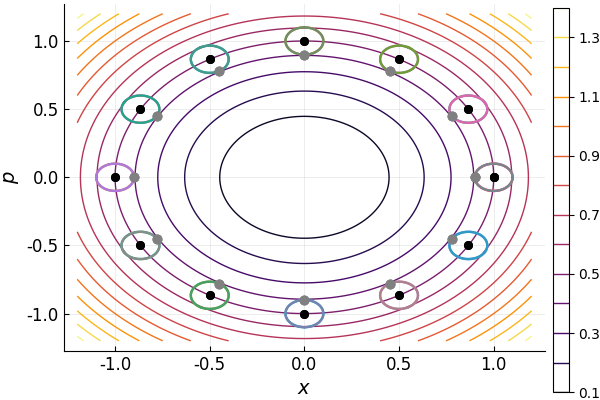
\includegraphics[width=0.8\linewidth]{oscillator_phsp}
 \caption{Espacio fase para el oscilador armónico representado por la ecuación \ref{eq:oscilador_ham}. En negro aparece la solución calculada con el método de Taylor para jets con $\xo = (1,0)^T$, tolerancia $\epsilon_{Taylor} = 10^{-20}$, orden de la expansión $M = 28$ y orden del jet $N=4$. Los jets fueron evaluados para la vecindad parametrizada por $\mathbf{\xi}(\tau) = 0.1\cdot \left( \cos(\tau), \sin(\tau) \right)^T$, $\tau \in [0,1]$, mientras que la solución en gris representa la variación $\xi = (-0.1,0)^T$.}
 \label{fig:oscilador_phsp}
\end{figure}

Así, tenemos que las soluciones analíticas son de la forma 
\begin{align}
 x(t) &= v_{0}\sin{(\omega t)} + x_{0}\cos{(\omega t)} \nonumber \\ 
 v(t) &= v_{0}\omega\cos{(\omega t)} - x_{0}\omega\sin{(\omega t)}. 
 \label{eq:oscilador_analytical}
\end{align}

La figura \ref{fig:oscilador_phsp} presenta al espacio fase del oscilador armónico, junto con una solución calculada con el transporte de jets. En ésta se observa cómo las soluciones evaluadas en una vecindad inicial parametrizada por un círculo están siempre en las líneas de las curvas de nivel del hamiltoniano. Se observa además en la figura la estructura de centros alrededor del único punto singular $(0,0)^T$.

Dada la condición inicial $\xo = (1,0)^T$ y tomando $m = 1 \ Kg$, $k = 1 \frac{Kg}{s^2}$, el oscilador tendrá una energía de $E_0 = H(\xo) = 1$ Joules. En la figura \ref{fig:oscillator_deltas} se pueden ver las variaciones $\delta E(t_n)$ de la energía en cada paso de integración así como la diferencia $\delta \mathbf{x}(t_n)$ de las soluciones de jet calculadas por el método de Taylor evaluadas en diferentes $\xi$s y las soluciones analíticas del oscilador armónico correspondientes al desplazamiento dado por dichas $\xi$s.

%FIGURA!
 \begin{figure}[h!]
\centering
\begin{subfigure}{0.49\textwidth}
	\centering
	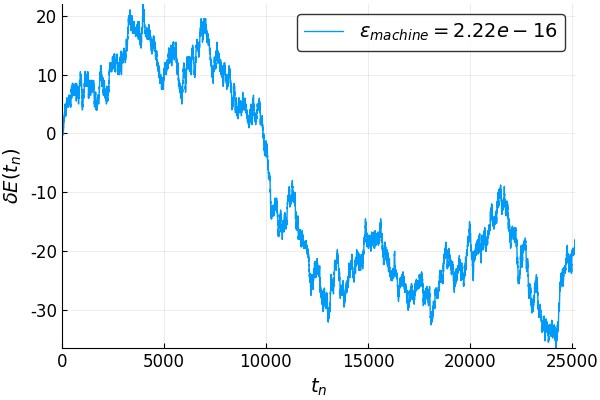
\includegraphics[width = \textwidth]{oscillator_dE}
	\caption{Variación $\delta E(t_n) = \frac{E(t_n)-E_0}{\epsilon_{machine}}$ de la energía respecto a la energía inicial $E_0 = 1$ Joule.\\ \\ }
	\label{fig:oscillator_dE}
\end{subfigure}
%
\begin{subfigure}{0.49\textwidth}
	\centering
	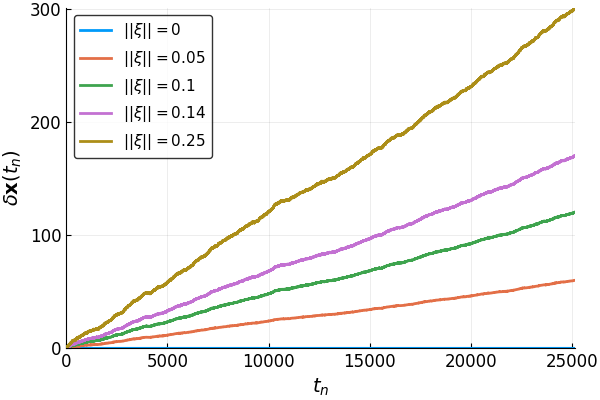
\includegraphics[width = \textwidth]{oscillator_dx}
	\caption{Variación $\delta \mathbf{x}(t) =  \frac{\norm{\mathbf{x}(t_n) - \mathbf{x_n}}_2}{\epsilon_{machine}}$ respecto a la solución analítica (\ref{eq:oscilador_analytical}) para distintos desplazamientos $\xi$ respecto de la condición inicial $\xo$.}
	\label{fig:oscillator_dx}
\end{subfigure}
\caption{Variaciones de energía y trayectoria para el oscilador armónico en cada uno de los pasos temporales de la solución con condición inicial $\xo = (1,0)^T$ y vecindad parametrizada por  $\mathbf{\xi}(\tau) = 0.1\cdot \left( \cos(\tau), \sin(\tau) \right)^T$, $\tau \in [0,1]$. Se utilizó tolerancia $\epsilon_{Taylor} = 10^{-20}$, orden de la expansión $M = 28$ y orden del jet $N=4$.}
\label{fig:oscillator_deltas}
\end{figure}

Es interesante notar que (\ref{eq:oscilador_ode}) es un sistema lineal de ecuaciones y, por tanto, basta con un jet de orden $1$ para obtener la mejor aproximación de las vecindades de $\xo$. De hecho, evaluar $\U_{\xo}$ en $f(\mathbf{x})$ de (\ref{eq:ode}) siempre regresa una cantidad lineal y por tanto, nunca aparecen términos de orden mayor en las variables del sistema de EDO.

\subsubsection{Péndulo simple}
\label{sec:pendulo}
Sea un sistema donde una masa $m$ está anclada al extremo de una varilla de longitud $l$ cuya masa es despreciable. Esta varilla está anclada, a su vez, a un punto inmovil. Así, $m$ se mueve bajo la acción de la gravedad $\mathbf{g}$ como se muestra en la figura \ref{fig:pendulo}, ignorando la resistencia del aire.

%FIGURA! 


La forma más natural de trabajar este problema es en coordenadas polares, en donde la masa $m$ se mueve con una velocidad $v = l\dot{\theta}$ con $l$ constante, es decir $r = l \neq r(t) \implies \dot{r} = \dot{p_r} = 0$. Esta constricción reduce en uno los grados de libertad del sistema, haciendo que éste dependa únicamente de $\theta$. 

Tenemos que 
\begin{align}
 K &= \frac{1}{2}m v^2 = \frac{1}{2} m l^2 \dot{\theta}^2 \nonumber \\
 U &= mgh(\theta) = mgl\left(1 - \cos{\theta} \right)
\end{align}
son la energía cinética y potencial, respectivamente. 

Así, contruimos el lagrangiano del sistema
\begin{equation*}
 \mathcal{L}(\theta,\dot{\theta}) = K - U = \frac{1}{2} m l^2 \dot{\theta}^2 - mgl\left(1 - \cos{\theta} \right).
\end{equation*}
Sabemos, por (\ref{eq:lagr-ham-rel}), que
\begin{equation*}
 \mathbf{p} = \frac{\partial \mathcal{L}}{\partial \mathbf{\dot{q}}} = ml^2\dot{\theta}
\end{equation*}

obteniendo la coordenada conjugada de momento y, así, plantear el hamiltoniano, o energía total del sistema, como
\begin{equation}
 H(p,\theta) = K + U = \frac{p_{\theta}^2}{2ml^2} + mgl\left(1 - \cos{\theta} \right).
\label{eq:pendulo-ham}
\end{equation}
 
Las EDO quedan entonces, por (\ref{eq:ham-rel}), como
\begin{align}
 \dot{\theta} &= \frac{p_{\theta}}{ml^2} \nonumber \\
 \dot{p_{\theta}} &= -mgl\sin{\theta} 
\label{eq:pendulo-ode}
\end{align}

en cuyo dominio $(\theta,p_{\theta}) \in [-\pi,\pi]\times[p_{min},p_{max}] \subset \mathbb{R}^2$ existen tres puntos singulares: $(-\pi,0),(\pi,0), (0,0)$; dos puntos de ``liberación'' y otro de ``relajación'', respectivamente. En la figura \ref{fig:pendulum_pshp} se puede ver una representación del espacio fase donde se exhibe el comportamiento de dichos puntos.

%FIGURA!
\begin{figure}[h!]
 \centering
 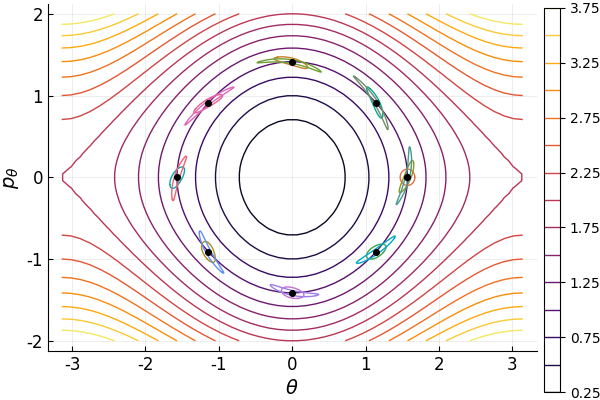
\includegraphics[width=0.8\linewidth]{pendulum_phsp}
 \caption{Espacio fase para el péndulo simple representado por la ecuación \ref{eq:pendulo-ham}. En negro salen puntos de la trayectoria calculada con el método de Taylor para Jets con $\xo = (\frac{\pi}{2},0)^T$, tolerancia $\epsilon_{Taylor} = 10^{-20}$, orden de la expansión $M = 28$ y sus vecindades (jets) evaluadas para $\mathbf{\xi}(\tau) = 0.1\cdot \left( \cos(\tau), \sin(\tau) \right)^T$, $\tau \in [0,1]$.}
\label{fig:pendulum_pshp}
\end{figure}

Si viajamos a un planeta en donde $g = 1 \ \frac{m}{s^2}$ \footnote{A veces, para la física, es más fácil viajar a un planeta donde exista la atracción gravitacional que más nos gusta que hacer a un péndulo girar en la Tierra; qué comodo.} y tomamos una varilla de longitud $l=1$ m y una masa $m=1$ kg,  entonces, para las condiciones iniciales $p_{\theta}(0) = 0 \ N \cdot m$ y $\theta(0) = \pi/2$, la energía total es 
\begin{equation*}
E_0 = H(p_{\theta}(0),\theta (0) ) = 1 \text{ J.}
\end{equation*}

Para dichas condiciones, se puede integrar el transporte de jets y además, evaluarlo para condiciones cercanas y ver cómo se comportan éstas soluciones en el espacio fase, que deben, en teoría, moverse por las curvas de (\ref{eq:pendulo-ham}). Se puede observar de la figura \ref{fig:pendulum_jt_O4} cómo para jets de orden 4, las soluciones se quedan sobre las curvas de nivel del hamiltoniano.

%FIGURA!
\begin{figure}[h!]
\centering
\begin{subfigure}{0.49\textwidth}
	\centering
	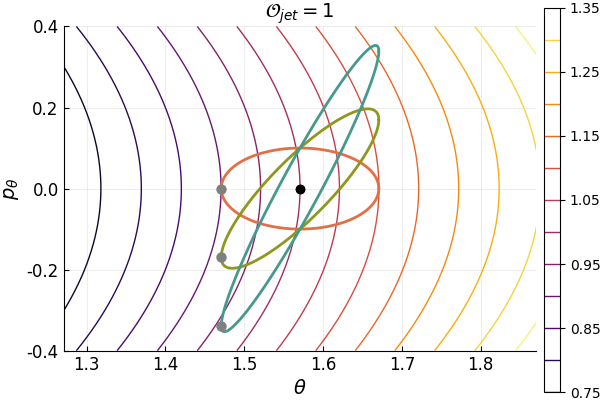
\includegraphics[width = \textwidth]{pendulum_jt_O1}
	\caption{Jet de orden $1$ después de dos periodos desde $\xo$.}
	\label{fig:pendulum_jt_O1}
\end{subfigure}
%
\begin{subfigure}{0.49\textwidth}
	\centering
	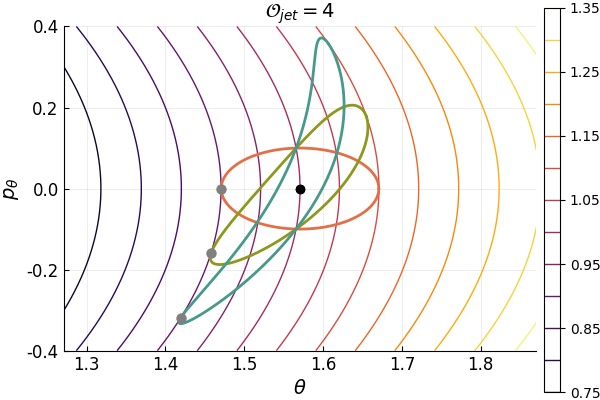
\includegraphics[width = \textwidth]{pendulum_jt_O4}
	\caption{Jet de orden $4$ después de dos periodos desde $\xo$.}
	\label{fig:pendulum_jt_O4}
\end{subfigure}
\caption{Jets de distinto orden para $\U_{\xo}$ parametrizada en un círculo de radio 0.1 $\mathbf{\xi}(\tau) = 0.1\left( \cos(\tau),\sin(\tau) \right)^T$ alrededor de $\xo = (\frac{\pi}{2},0)^T$ en el péndulo simple. Se utilizó tolerancia $\epsilon_{Taylor} = 10^{-20}$ y orden de la expansión $M = 28$.}
\label{fig:pendulum_jt}
\end{figure}

Respecto a las variaciones de energía en el sistema, se ve en la figura \ref{fig:pendulum_dE} cómo $\delta E(t)$ varía alrededor de cero como un movimiento browniano. Éste último se relaciona con los errores de redondeo de puntos flotantes de la máquina y no con el método de Taylor en sí, a diferencia del método de Euler, como se observa en la figura \ref{fig:center_anal_comparison}, donde el error crece de manera lineal. La máxima variación respecto a la energía inicial es de $2.28\times10^{-14}$, lo cual corresponde a $103 \epsilon_{machine}$ (sin redondear).

%FIGURA! 
\begin{figure}[h!]
 \centering
 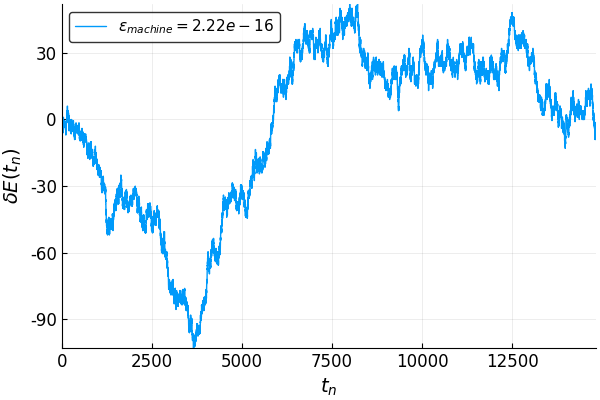
\includegraphics[width=0.8\linewidth]{pendulum_dE}
 \caption{Diferencia $\delta E(t_n) := \frac{E(t_n) - E_0}{\epsilon_{machine}}$ de la energía del péndulo simple con condición inicial $\xo = (\frac{\pi}{2},0)$, tolerancia $\epsilon_{Taylor} = 10^{-20}$ y orden de la expansión $M = 28$.}
 \label{fig:pendulum_dE}
\end{figure}

\subsubsection{Hamiltoniano Artificial}
\label{sec:artificial_ham}

Inventemos un hamiltoniano que no necesariamente represente un sistema físico. Éste último ejemplo servirá como motivación de la sección siguiente, ya que estaremos analizando las soluciones cerca de una curva límite y se podrá extender un poco la discusión sobre los jets y la necesidad de contruir algunos indicadores dinámicos relevantes. 

Sea 
\begin{equation}
 H(q,p) = qp^2 - \frac{1}{2}q^2
 \label{eq:artificial_ham}
\end{equation}

el hamiltoniano del sistema cuyas curvas de nivel representan las soluciones para la EDO
\begin{align}
 \dot{q} &= 2qp \nonumber \\
 \dot{p} &= -p^2 + q.
 \label{eq:artificial_ode}
\end{align}


Notemos que el sistema anterior tiene un único punto singular $(0,0)^T$ que corresponde a una energía de $H(0,0) = 0$. Con esto, podemos obtener la condición para que las soluciones estén sobre dicho curva límite o separatriz que divide diferentes regiones del espacio. Vemos que si
\begin{equation*}
 H(q,p) = qp^2 - \frac{1}{2}q^2 = 0 \implies p = \pm \sqrt{\frac{q}{2}} 
\end{equation*}

entonces las condiciones iniciales tipo $\xo = \left( q, -\sqrt{\frac{q}{2}} \right)$ vivirán sobre la separatriz. 

%FIGURA!
\begin{figure}[h!]
 \centering
 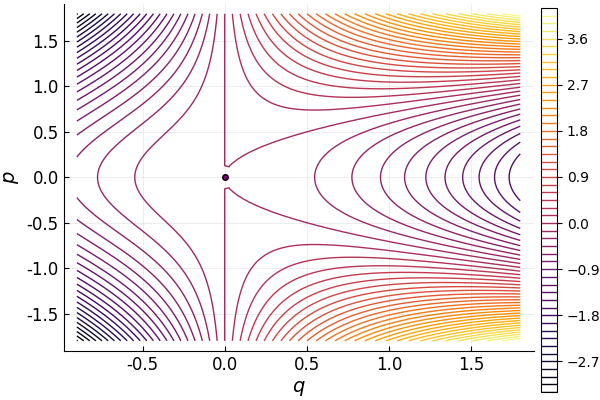
\includegraphics[width= 0.8\linewidth]{artificial_phsp}
 \caption{Espacio fase de \ref{eq:artificial_ode}.}
 \label{fig:artificial_phsp}
\end{figure}

Se muestra en la figura \ref{fig:artificial_phsp} el espacio fase dado por el hamiltoniano del sistema. Notemos que dicha separatriz se puede observar como una especie de parábola horizontal positiva con centro en el punto singular.

%FIGURA!
\begin{figure}[h!]
 \centering
 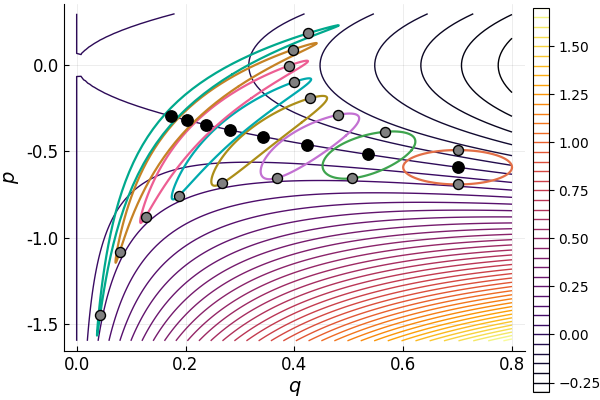
\includegraphics[width= 0.8\linewidth]{artificial_jt_O16}
 \caption{Solución para (\ref{eq:artificial_ode}), con condición inicial sobre la separatriz, donde $q_0 = 0.7$. Aquí, los jets son de orden $M=16$, en $8$ pasos de integración desde $t_0 = 0$ hasta $t_{max} = 1.7$, con tolerancia $\epsilon_{Taylor} = 10^-{20}$ y orden de la expansión $N=28$. En gris están las soluciones a $\xo + \xi$ sin utilizar TJ.}
 \label{fig:artificial_jt}
\end{figure}

Si tomamos $q_0 = 0.7$ con la condición anterior, y hacemos un transporte de jets alrededor de dicha condición inicial podríamos ver, en teoría, las trayectorias que toman las soluciones cercanas a la curva límite en cada lado de la frontera que ésta impone. En la figura \ref{fig:artificial_jt} se observa la deformación de estos jets conforme pasa el tiempo y, aunque la evolución temporal es un intervalo relativamente corto, es evidente la tendencia que tienen las soluciones cercanas a diverger.

En este problema se vuelve importante muy rápidamente la precisión con la que los jets nos dan soluciones cercanas ya que la deformación de la vecindad inicial $\U_{\xo}$ es muy grande. Por esto, se muestra en la tabla \ref{table:djet_artificial} la diferencia entre evaluar el jet en $\xi = (0,-0.1)^T$ y hacer el método de Taylor convencional partiendo de ese punto. De hecho, se observan en la figura \ref{fig:artificial_jO2_jO16} la evaluación de jets de distinto orden para la misma vecindad inicial alrededor de $\xo$.

%TABLA!
\begin{table}[h!]
\centering
\begin{tabular}{c|ccccc}
\toprule
               & \textbf{$ M = 1 $} & \textbf{$M = 2 $} & \textbf{$ M = 4$} & \textbf{$ M = 8 $} & \textbf{$ M = 16 $} \\ \cmidrule(l){1-6} 
\textbf{$t_0$} & -Inf                       & -Inf                       & -Inf                       & -Inf                       & -Inf                          \\
\textbf{$t_1$} & -2.42                      & -3.97                      & -7.07                      & -13.28                     & -15.95                        \\
\textbf{$t_2$} & -1.92                      & -3.1                       & -5.47                      & -10.22                     & -15.95                        \\
\textbf{$t_3$} & -1.54                      & -2.48                      & -4.37                      & -8.15                      & -15.91                        \\
\textbf{$t_4$} & -1.21                      & -1.96                      & -3.47                      & -6.49                      & -12.53                        \\
\textbf{$t_5$} & -0.91                      & -1.49                      & -2.68                      & -5.05                      & -9.79                         \\
\textbf{$t_6$} & -0.61                      & -1.05                      & -1.95                      & -3.74                      & -7.34                         \\
\textbf{$t_7$} & -0.29                      & -0.6                       & -1.24                      & -2.52                      & -5.08                         \\ \bottomrule 
\end{tabular}
\caption{Diferencia logarítmica de $\delta \mathbf{x} = \norm{ \phi(t_i,t_0,\xo + (0,-0,1)^T) - P_{i,\xo}((0,-0.1)^T) }$ para polinomios $P_{i,\xo}(\xi)$ de distinto orden $M$ en $\xi$.}
\label{table:djet_artificial}
\end{table}

%FIGURA!
\begin{figure}[h!]
 \centering
 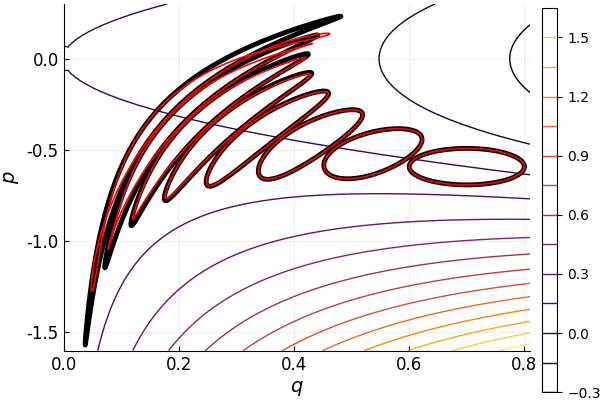
\includegraphics[width= 0.7\linewidth]{artificial_jO2_jO16}
 \caption{Diferencia gráfica entre un jet de orden $M=2$ contra uno de orden $M=16$ para las mismas condiciones.}
 \label{fig:artificial_jO2_jO16}
\end{figure}

Recordemos que como (\ref{eq:artificial_ode}) es un sistema de EDO hamiltoniano entonces deberá conservar la energía. En la figura \ref{fig:artificial_dE} se observa la variación de la energía para cada paso temporal con el jet evaluado en $\xi = (0,\pm 0.1)^T$, así como en $\xo$, i.e., para el método de Taylor sin jets. Notemos cómo al principio (figura \ref{fig:artificial_dEjets_half}) la energía sí se conserva, i.e, las evaluaciones del TJ se mantienen sobre las superficies de nivel del hamiltoniano, sin embargo, cuando la vecindad se empieza a deformar más, la energía empieza a variar más respecto a la de su condición inicial. Notemos que aunque esta variación es de $\approx 10^8 \epsilon_{machine}$, el error en la energía es en la octava cifra significativa, dado que $\epsilon_{machine} = 2.22\times 10^{-16}$.

%FIGURA!
\begin{figure}[h!]
 \centering
 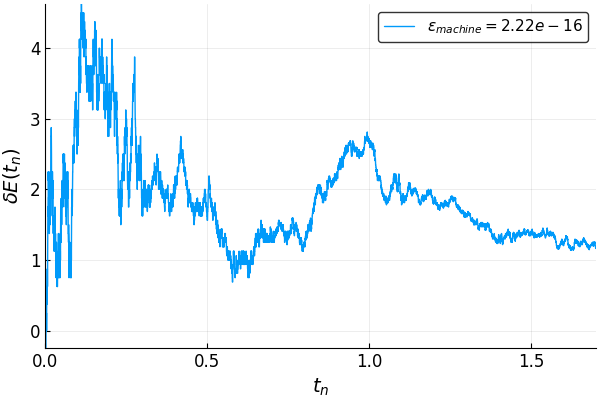
\includegraphics[width=0.7\linewidth]{artificial_dE}
 \caption{Diferencia en energía $\delta E(t_n) = \frac{1}{\epsilon_{machine}} \left( H(\mathbf{x}(t_n)) - H(\xo) \right)$ para el sistema \ref{eq:artificial_ode} sin transporte de jets, con tolerancia $\epsilon_{Taylor} = 10^{-20}$, orden de expansión $N = 28$ y $8000$ pasos temporales de $t_0 = 0$ a $t_{max} = 1.7$.}
 \label{fig:artificial_dE}
\end{figure}

%FIGURA!
\begin{figure}[h!]
\centering
\begin{subfigure}{0.49\textwidth}
	\centering
	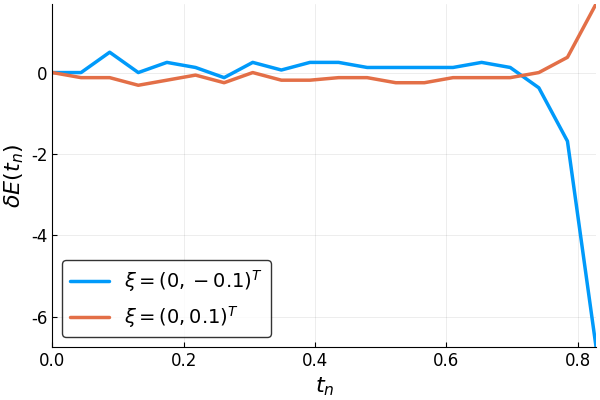
\includegraphics[width = \textwidth]{artificial_dEjets_half}
	\caption{Diferencias de energía $\delta E$ respecto a la energía inicial en la primera mitad de la integración.}
	\label{fig:artificial_dEjets_half}
\end{subfigure}
%
\begin{subfigure}{0.49\textwidth}
	\centering
	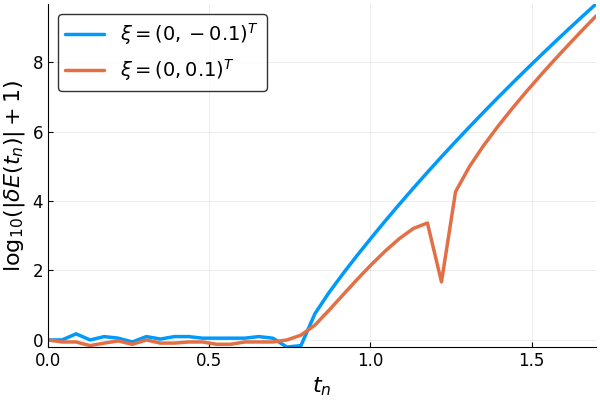
\includegraphics[width = \textwidth]{artificial_dEjets_all}
	\caption{Logaritmo de las diferencias de energía $\delta E$ respecto a la energía inicial en toda la integración.}
	\label{fig:artificial_dEjets_all}
\end{subfigure}
\caption{Diferencia en energía $\delta E(t_n) = \frac{1}{\epsilon_{machine}} \left( H(\mathbf{x}(t_n)) - H(\xo) \right)$ para el sistema (\ref{eq:artificial_ode}) con jets de orden $M=16$ evaluados en $\xi$. Se utilizó tolerancia $\epsilon_{Taylor} = 10^{-20}$, orden de expansión $N = 28$ y $40$ pasos temporales de $t_0 = 0$ a $t_{max} = 1.7$.}
\label{fig:artificial_dEjets}
\end{figure}


Todos los ejemplos construidos en la última sección han sido evaluados en una vecindad con un radio de $r = 0.1$ alrededor de $\xo$. Sin embargo, nada asegura que ésta sea una buena elección para dicha vecindad. Estudiar cuál es el tamaño máximo que una vecindad puede tomar para que los jets arrojen soluciones precisas se vuelve una pregunta natural al ver las gráficas y tablas de éstos ejemplos. Por otro lado, hemos visto en éste último ejemplo cómo una vecindad inicial puede deformarse bastante rápido cerca de una curva límite cuando en el oscilador armónico, en cambio, no se deforma nada. Establecer una métrica de deformación se vuelve, también, una forma de análisis del estudio de vecindades de alguna condición $\xo$ dada para algún sistema de ecuaciones diferenciales a trabajar. En el caso del péndulo simple, se observa cómo después de cada periodo de oscilación, el jet se deforma de manera tal que las soluciones cercanas no cruzan la condición inicial al mismo tiempo que $\xo$; esto se puede estudiar si pintamos una sección transversal a las soluciones del péndulo que pase por $xo$ y observamos en qué tiempo cruzan las vecindades ésta sección. El uso de jets motiva a hacer varios indicadores sobre la dinámica de las ecuaciones son obtener explícitamente la solución. Es importante notar que no siempre se tendrá un hamiltoniano explicito para comparar las soluciones con sus curvas de nivel, así que estos indicadores servirán para darnos información sobre el espacio fase sin conocerlo del todo. 

%Los siguientes indicadores están motivados fuertemente en lo discutido en \cite{Perez2015}, \cite{Perez2015}, \cite{Haro2009}.

%% Para que de nuevo haya salto de linea. (buscar Dutch style)
\setlength{\parskip}{1.3ex plus 0.2ex minus 0.2ex}

\chapter{Indicadores Dinámicos del TJ} 
\label{chap:jt_indicators}
En los ejemplos anteriores se ha evaluado la precisión del método de Taylor con y sin el transporte de jets. Hemos estudiado casos hamiltonianos en donde las soluciones a las ecuaciones diferenciales viven en curvas de energía constante sobre el espacio fase. Es importante tener en cuenta que éste es sólo un subconjunto de casos en la familia de sistemas de ecuaciones diferenciales ordinarias. Nuevos elementos aparecen en los campos vectoriales impuestos por la forma más general de (\ref{eq:ode}) como órbitas periódicas, atractores, repulsores o atractores extraños \cite{Perez2015}. La idea de los indicadores dinámicos radica en encontrar estructuras que nos permitan catalogar a los campos vectoriales, sean hamiltonianos o no, y sacar información relevante acerca de las soluciones al sistema de ecuaciones dado. 

Hay que destacar que el transporte de jets no sirve únicamente para dar indicadores dinámicos del espacio fase. Hay un montón de cosas que se pueden aprovechar al tener la solución parametrizada por polinomios. Entre éstas están hacer simulaciones de Montecarlo o hacer variación de los parametros de las ecuaciones.

\subsection{Un poco de motivación vía exponentes de Lyapunov}
\label{sec:FTLE}

El transporte de jets nos permite saber qué pasa con el flujo entre condiciones iniciales vecinas. En este sentido, si se hace un transporte alrededor de $\xo$, sabemos como es el flujo de $\xo + \delta \xo$. Por esto, los Exponentes de Liapunov a Tiempo Finito (ELTF) emergen commo una motivación natural a los indicadores que serán propuestos en este capítulo. Un ELTF es, sin entrar en muchos detalles, el promedio en un lapso finito de tiempo de la tasa de máxima expansión entre dos condiciones iniciales cercanas. La construcción que aquí se plantea sigue a Shadden, Lekien y Marsden en \cite{Shadden2005}.

Supongamos dos condiciones iniciales vecinas $\xo$ y $\mathbf{\chi}_0 = \xo + \delta \xo$ en $\mathcal{D} \subset R^d$ con flujos $\phi(T;t_0, \xo)$ y $\phi(T;t_0, \chi_0)$, respectivamente, después de un intervalo $T$ de tiempo, con $\delta \xo \ll 1$ y en alguna dirección arbitraria . La perturbación después del intervalo $T$ es

\begin{equation}
 \delta \mathbf{x}(T) = \phi(T;t_0, \chi_0) - \phi(T;t_0, \xo) = \frac{d \phi(T;t_0, \xo)}{d\xo} \delta \xo + \mathcal{O} \left( \norm{ \delta \xo}^2 \right).
 \label{eq:perturbation}
\end{equation}

Ignorando el término de orden cuadrático en $\delta \xo$, se puede encontrar la magnitud de la perturbación al tiempo $T$ via la norma estándar

\begin{equation}
 \norm{\delta \mathbf{x}(T)} = \sqrt{ \left\langle \frac{d \phi(T;t_0, \xo)}{d\xo} \delta \xo, \frac{d \phi(T;t_0, \xo)}{d\xo} \delta \xo \right\rangle }.
 \label{eq:perturbation_norm}
\end{equation}

La máxima expansión de (\ref{eq:perturbation_norm}), se encuentra en la dirección donde $\delta \xo$ esté alineada con el eigenvector asociado al máximo eigenvalor de la matriz\footnote{Esta matriz se suele conocer como el tensor (derecho) de Cauchy-Green.}
\begin{equation}
 \Lambda(\xo, T) := \frac{d \phi(T;t_0, \xo)}{d\xo}^* \frac{d \phi(T;t_0, \xo)}{d\xo}.
 \label{eq:finite_cgtensor} 
\end{equation}
Es decir, 
\begin{equation*}
 \max_{\delta \xo} \norm{\delta \mathbf{x}(T) } = \sqrt{ \lambda_{max}(\Lambda) \norm{ \delta \tilde{\xo}}^2 } = e^{\sigma(\xo,T)\lvert T \rvert} \norm{ \delta \tilde{\xo} }  ,
\end{equation*}
con $ \delta \tilde{\xo} $ en la dirección del eigenvector asociado a $\lambda_{max}(\Lambda)$ y
\begin{equation}
 \sigma(\xo,T) := \frac{1}{2 \lvert T \rvert} \ln \lambda_{max}(\Lambda(\xo, T)),
 \label{eq:FTLE}
\end{equation}
el máximo ELTF integrado a tiempo $T$ asociado al punto que en $t_0$ pasa por $\xo$. Como se mencionaba al principio de la sección, $\sigma(\xo,T)$ nos da la tasa de máxima expansión de $\xo$ promediada en el intervalo $T$. Calcular el ELTF es fácil con el TJ ya que, por la parametrización polinomial de $\flowxi$, $\lambda(\xo,T)$ se puede calcular directamente usando jets de orden $M = 1$. Con esto, se puede estudiar al espacio fase de una campo vectorial dado ya que diferentes valores de $\sigma$ representan diferentes tasas de expansión para la misma escala temporal.

%FIGURA!
\begin{figure}[h!]
 \centering
 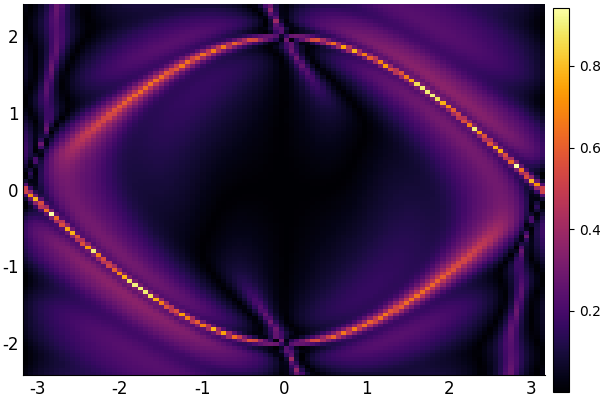
\includegraphics[width=0.7\linewidth]{ftle_pendulum}
 \caption{Campo escalar de los ELTF para el péndulo de (\ref{eq:pendulo-ode}) en una retícula de $100$ puntos por lado, después de un periodo, con tolerancia $\epsilon_{Taylor} = 10^{-10}$ y orden máximo de la expansión $M = 25$.}
 \label{fig:ftle_pendulum}
\end{figure}

La figura \ref{fig:ftle_pendulum} presenta al campo escalar de los ELTF calculados a partir de (\ref{eq:FTLE}) para el péndulo simple descrito por (\ref{eq:pendulo-ode}). Es interesante cómo la separatrices del péndulo coinciden con los valores más grandes de $\sigma$ en el espacio fase. En \cite{Haller2011}, se hace un análisis profundo para detectar diferentes regiones en el espacio fase, que ahí nombra como Estructuras Lagrangianas Coherentes, motivado en la parcelas lagrangianas de la mecánica de fluidos. Como se muestra en la referencia anterior, no necesariamente el campo escalar de ELTF va a encontrar separatrices, sino puntos cuyas soluciones vecinas se alejan rápidamente en el tiempo; esto puede indicar, sí, separatrices, pero también caos, o grandes gradientes de velocidad en el espacio fase.

%Casos donde esto falla o donde el jacobiano no es suficientemente buena aproximación... 

\pagebreak

\subsection{Tamaño máximo de las vecindades}
%
%Vimos, en el caso anterior, cómo el jacobiano $J^{t_n}(\xi)$ representa la deformación lineal de las trayectorias vecinas a $\xo$ al tiempo $t_n$ y cómo, con éste, se puede calcular el campo escalar de los ELTF. Sin embargo, en los ejemplos XXX se observa que a veces la aproximación lineal de las deformaciones no es suficiente para sacar conclusiones contundentes sobre el sistema de EDO. De hecho, por el teorema de Grobman-Hartman, existen casos donde las ecuaciones no son siquiera topológicamente equivalentes a su aproximación lineal. 
%%Trabajar los ejemplos XXX.

Los ELTF son una buena herramienta para ver la tasa de expansión de la variacion entre dos condiciones vecinas. Esto es una buena motivante para el transporte de jets, ya que no se tiene, a priori, la restricción de la linealidad que se tiene en el caso anterior. Lo único que se hizo para adaptar el TJ al campo de ELTF fue tomar una expansión a primer orden de las soluciones de un campo vectorial dado. Sin embargo, si las expansiones de los polinomios son de orden $N > 1$, entonces las deformaciones en las vecindades de $\xo$ exhibirán términos no lineales para cada término del flujo y, así, se puede obtener información más precisa con los indicadores pertinentes\footnote{La figura \ref{fig:pendulum_jt} es un buen ejemplo de cómo no siempre las deformaciones lineales son suficientes si la variación es suficientemente grande.}. Intuitivamente, entre mayor sea el orden de expansión de los jets, mejor será la aproximación a la solución real en las vecindades de $\xo$ y más grandes pueden ser las variaciones respecto a $\xo$; sin embargo, no se ha analizado qué tan grandes deben ser dichas variaciones para estar bajo una tolerancia impuesta.

%FIGURA!
\begin{figure}[h!]
	\centering
	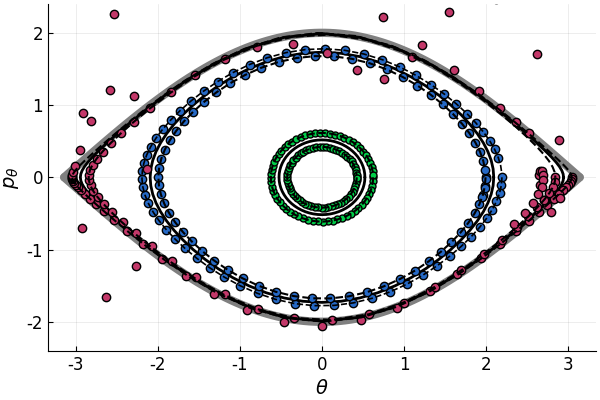
\includegraphics[width=0.7\linewidth]{xi_precision_pendulum}
	\caption{Evaluación del TJ para $\xi = ( \pm 0.1, 0)^T$ en un periodo del péndulo simple en tres distintas secciones para una tolerancia $\epsilon_{Taylor} = 10^{-10}$, jets de orden $M=4$ y expansión de orden $N=24$ Las integraciones nominales de $\xo \pm \xi$ se representan con las curvas negras no sólidas, mientras que la integración para $\xo$ son las curvas negras sólidas. \textit{En verde}: $\xo = (\pi/6, 0)^T$, \textit{En azul}: $\xo = (2\pi/3, 0)^T$ y \textit{En rosa}: $\xo = (15\pi/16, 0)^T$.}
	\label{fig:xi_precision_pendulum}
\end{figure}

%FIGURA! 
%\begin{figure}[h!]
%\centering
%\begin{subfigure}{0.49\textwidth}
%	\centering
%	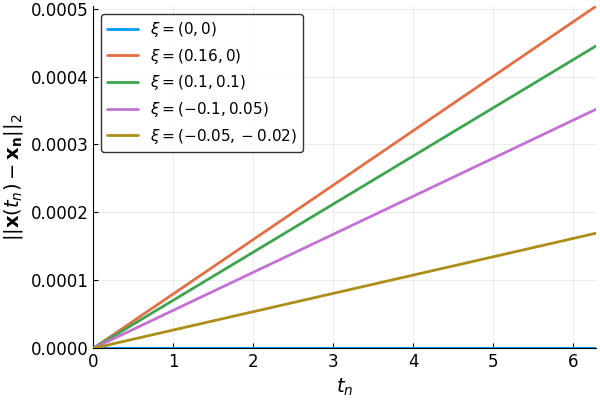
\includegraphics[width = \textwidth]{euler-vs-analytical_center}
%	\caption{Norma de la diferencia entre la solución real y evaluaciones de la solución numérica para distintos valores de $\xi$ marcados en la gráfica. Se puede observar un crecimiento lineal del error numérico, lo cual es una de las consecuencias de usar el método de Euler.}
%	\label{fig:center-eu_vs_anal}
%\end{subfigure}
%%
%\begin{subfigure}{0.49\textwidth}
%	\centering
%	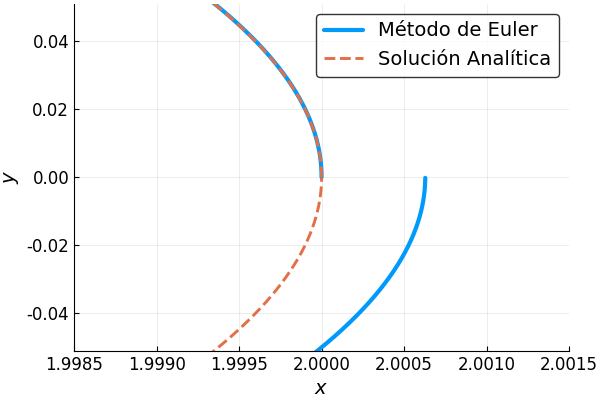
\includegraphics[width = \textwidth]{euler-method_error}
%	\caption{Sección del espacio fase donde se observan la solución analítica y la solución numérica para pasos de $h=10^{-4}$ con cóndición inicial $\xo = (2,0)$. \\ \\}

Los coeficientes de la expansión de $\flowxi$ dependen de qué tan grandes son las variaciones de las vecindades de la condición tomada para el flujo. La figura \ref{fig:xi_precision_pendulum} muestra cómo para la misma variación $\xi = (\pm 0.1, 0)^T$ el transporte no siempre se comporta de la manera. Más cerca de la separatriz, las evaluaciones se parecen uy poco a flujo real. Así, una forma de controlar qué tan grandes pueden ser las variaciones alrededor de $\xo$ es acotar la contribución del último término a una tolerancia dada; es decir,
\begin{equation*}
 a_{M}^{(n)}\xi_{max}^M \leq \epsilon_{jet}
\end{equation*}
donde $\flowxi = P_{n,\xo}(\xi) = \sum_{|m|=1}^M  a_{m}^{(n)} \xi^m$, con $a_{m}^{(n)}$ el polinomio de orden $m = \norm{\mathbf{m}}_1$ del jet al tiempo $t_n$.

Se busca controlar el máximo de estos coeficientes, de modo que 
\begin{align}
 \xi_{max} = \min_{|m|=M} \left( \frac{\epsilon_{jet}}{a_{m}^{(n)}} \right)^{\frac{1}{m}}.
 \label{eq:ximax}
\end{align}
es el radio máximo que la vecindad $\Uxo$ puede tomar para estar debajo de la tolerancia impuesta. 

Con ésto se establece qué tan grandes pueden ser las variaciones de $\xo$ sin que las deformaciones del jet repercutan de manera drástica en las soluciones evaluadas. La sección \ref{sec:artificial_ham} muestra cómo la dinámica del campo vectorial exige que las deformaciones de $\Uxo$ sean muy grandes y, como se observó en la figura \ref{fig:artificial_dEjets_all}, después de cierto tiempo la energía deja de conservarse, lo cual implica que la solución ya no vive en la curva de nivel del hamiltoniano y, por tanto, el TJ no es suficiente preciso para determinar soluciones cercanas. Visto de otro ángulo, la vecindad en la que se evaluó era demasiado grande para conservar la energía en toda la trayectoria del flujo.

%FIGURA!
\begin{figure}[h!]
	\centering
	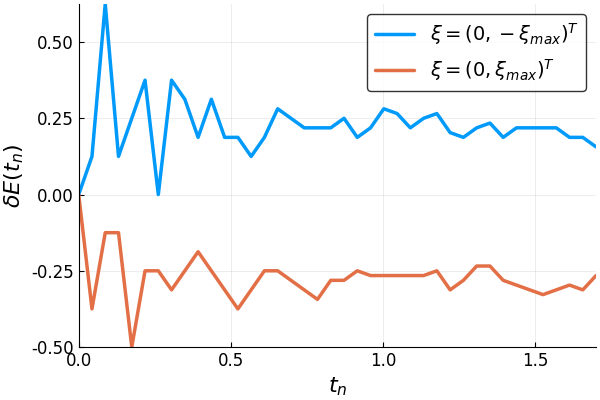
\includegraphics[width=0.7\linewidth]{dE_ximax_ah}
	\caption{Diferencia de energía $\delta E(t_n) = \frac{1}{\epsilon_{machine}} \left( H(\mathbf{x}(t_n)) - H(\xo) \right)$ para el sistema (\ref{eq:artificial_ode}) con jets de orden $M=16$ evaluados en $\xi_{max} = 0.0235$, el cual se calculó con $\epsilon_{jet} = 10^{-14}$. Se utilizó tolerancia $\epsilon_{Taylor} = 10^{-10}$, orden de expansión $N = 25$ y $40$ pasos temporales de $t_0 = 0$ a $t_{max} = 1.7$.}
	\label{fig:dE_ximax_ah}
\end{figure}

En la figura \ref{fig:dE_ximax_ah} retomamos al sistema (\ref{eq:artificial_ode}) que, en su momento, vimos cómo divirgió su energía. Ahora podemos ver que, al establecer una tolerancia $\epsilon_{jet} = 10^{-14}$, las variaciones de energía para ambos casos $\pm \xi_{max}$ son \textbf{más pequeñas que el épsilon de la máquina}. Esto implica que establecer un tamaño máximo de las vecindades reduce drásticamente el error de las soluciones calculadas. Esto, sin embargo, tiene un costo relativamente alto, ya que $\xi_{max} = 0.0235 \ll 0.1$, donde $0.1$ fue la variación respecto a $\xo$ que se había escogido arbitrariamente en la sección \ref{sec:benchmark-taylor}. 

$\xi_{max}$ depende fuertemente de la tolerancia $\epsilon_{jet}$ escogida y, más importante, de la condición inicial en donde se busque saber la variación máxima posible. En general, entre más se deforme el jet con la evolución del flujo, menores serán las vecindades en las que las evaluaciones de $\flowxi$ queden debajo de $\epsilon_{jet}$. Con esto en mente, el tamaño máximo de la vecindad puede servir como un indicador similar a los ELTF, ya que es sensible a la separación entre condiciones iniciales cercanas. El tamaño de vecindad va a detectar grandes gradientes de velocidades, presencia de separatrices en el espacio fase y regiones de caos en \textbf{órdenes no lineales de la vecindad de las soluciones}. Se muestra en la figura \ref{fig:jt_ximax_ah} cómo $\flowU$ consta de una $\Uxo$ considerablemente más pequeña que en \ref{fig:artificial_jt}.

%FIGURA!
\begin{figure}[h!]
 \centering
 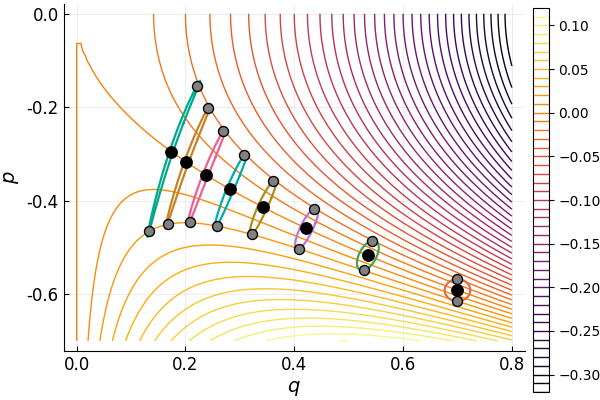
\includegraphics[width=0.7\linewidth]{jt_ximax_ah}
 \caption{Solución para (\ref{eq:artificial_ode}), con condición inicial sobre la separatriz, donde $q_0 = 0.7$. Aquí, los jets son de orden $M=16$, en $8$ pasos de integración desde $t_0 = 0$ hasta $t_{max} = 1.7$, evaluados para $\xi_{max} = 0.025$. Se utilizó tolerancia $\epsilon_{Taylor} = 10^-{20}$ y orden de la expansión $N=25$. En gris están las soluciones a $\xo \pm \xi_{max}$ sin utilizar TJ. La tolerancia para $\xi_{max}$ es de $\epsilon_{jet} = 10^{-5}$.}
 \label{fig:jt_ximax_ah}
\end{figure}

Dicho lo anterior, y a modo de comparar con los ELTF desarrollados previamente, tomemos el caso del péndulo simple, que tiene una separatriz que divide la zona en donde el péndulo oscila respecto a un punto de equilibrio (``rotación'') y la zona donde el péndulo completará períodos completos de oscilación (``libramiento'') . A diferencia de la figura \ref{fig:ftle_pendulum}, la figura \ref{fig:ximax_pendulum} alcanza sus mayores valores en el centro, que es donde las velocidades del campo vectorial son menores y, en cambio, en los valores de la separatriz, se alcanzan los mínimos valores para $\xi_{max}$, ya que es donde los jets sufren mayores deformaciones. Sin embargo, esta figura nos da información equivalente a los ELTF, ya que, cualitativamente, presenta la misma información y nos indica sobre la presencia de la separatriz. De hecho, si las no linealidades de $\xi_{max}$ no contribuyen de manera importante al cálculo de ésta, entonces $\xi_{max}(\xo,T) \propto \frac{1}{\sigma(\xo,T)}$. 

%FIGURA!
\begin{figure}[h!]
 \centering
 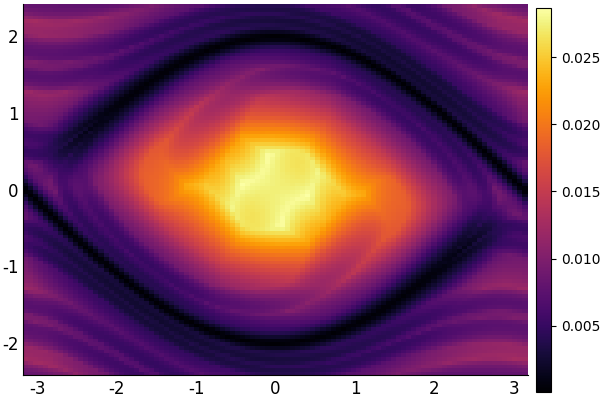
\includegraphics[width=0.7\linewidth]{ximax_pendulum}
 \caption{Campo escalar de los tamaños máximos de vecindad $\xi_{max}$ para el péndulo de (\ref{eq:pendulo-ode}) en una retícula de $60$ puntos por lado, después de un periodo, con tolerancia $\epsilon_{Taylor} = 10^{-10}$ y orden máximo de la expansión $M = 25$.}
 \label{fig:ximax_pendulum}
\end{figure}

%Hacer más ejemplo(s) con esto

\subsection{Tasa de expansión y contracción}
\label{sec:contraccion_expansion}

Otra forma de obtener información sobre los flujos es viendo la tasa de deformación de los jets propagados en el espacio fase. La ventaja de esto sobre el campo escalar de ELTF o del tamaño máximo de vecindades es que aquí es posible saber \textbf{en qué dirección} se tienen la mayor y menor deformación respecto a un punto en el espacio fase. Este indicador se relaciona, en este sentido, con el espectro de Lyapunov, que no es más que el conjunto de eigenvalores $\lambda_i$ obtenidos por las raíces del polinomio característico $P(\lambda) = \det(A - \lambda\mathbf{1})$. El espectro de Lyapunov nos dice cómo crece o se contrae la aproximación lineal de las soluciones bajo un cambio invertible de coordenadas. Las \textbf{tasas de expansión y contracción} de vecindades del flujo $\flowci$ ($\zeta_+$ y $\zeta_-$, respectivamente) nos dicen cuáles son la máxima y mínima separación de $\xo$ con una variación $\xi$ de radio $|\xi(\theta)| = \xi_{max}$.

Para obtener dicho indicador se hace el TJ del orden $M$ deseado integrando hasta $t = t_n$, se obtiene el radio máximo de la vecindad con el método de la sección anterior y se evalúa la frontera de $\Uxo$ en $P_{n,\xo}(\xi(\theta))$. Una vez evaluada, se encuentra el ángulo de máxima (mínima) separación 
\begin{equation}
 \theta_{+}(\xo) = \max_{\theta \in [0,2\pi)} \norm{ P_{n,\xo}(\xi(\theta)) - P_{n,\xo}(0) }
\end{equation} 
y se calcula 
\begin{equation}
 \zeta_{\pm}(\xo) = \frac{ \norm{P_{n,\xo}(\xi(\theta_{\pm})) - P_{n,\xo}(0)} }{\xi_{max}}.
 \label{eq:max_min_rate}
\end{equation}

En el caso de un grado de libertad, como los ejemplos hasta ahora planteados, se ha parametrizado dicha frontera con $\xi(\theta) = \xi_{max} \left( \cos(\theta), \sin(\theta) \right)^T, \theta \in [0,2\pi]$. Evidentemente no se puede evaluar la frontera de $\Uxo$ en un continuo de puntos en la computadora, así que se plantean dos maneras de mejorar la precisión sobre dichos máximos y mínimos: 
\begin{itemize}
\item Aumentar el número de puntos con los cuales se evalúa $\delta \Uxo$
\item Encontrar $\theta_{\pm}$ de los puntos disponibles y luego hacer un Newton-Rapson con $P_{n,\xo}$. 
\end{itemize} 

Se pueden encontrar $\theta_\pm$ y $\zeta_\pm$ para toda una rejilla de puntos y obtener dos campos vectoriales y dos escalares, respectivamente. Los campos vectoriales indican, para cada punto, la dirección de mayor y menor separación de la condición $\xo$ dada; los campos escalares indican la magnitud de esto último. En la figura \ref{fig:seprate_pendulum} se pueden ver ambos campos encimados para el péndulo simple donde, para cada punto de la rejilla, hay un vector en la dirección de máxima (mínima) separación y en color se indica la magnitud de dicha separación.

%FIGURA! 
\begin{figure}[h!]
\centering
\begin{subfigure}{0.49\textwidth}
	\centering
	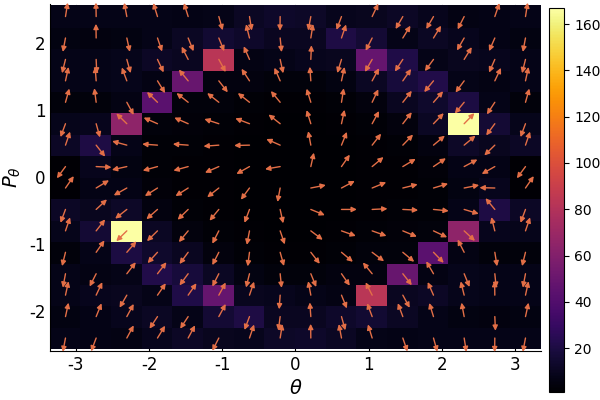
\includegraphics[width = \textwidth]{seprate_max_pendulum}
	\caption{Campos vectorial y escalar calculados con $\theta_+(\xo)$ y $\zeta_+(\xo)$,respectivamente.}
	\label{fig:seprate_max_pendulum}
\end{subfigure}
%
\begin{subfigure}{0.49\textwidth}
	\centering
	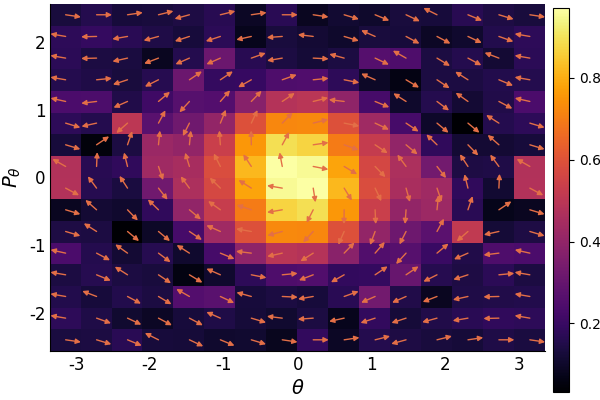
\includegraphics[width = \textwidth]{seprate_min_pendulum}
	\caption{Campos vectorial y escalar calculados con $\theta_-(\xo)$ y $\zeta_-(\xo)$,respectivamente.}
	\label{fig:seprate_min_pendulum}
\end{subfigure}
\caption{ Campos vectoriales dados por $\left( \cos(\theta_\pm(\xo)),\sin(\theta_\pm(\xo)) \right)^T$ sobre los campos escalares $\zeta_\pm(\xo)$ para el péndulo simple, en rejillas de $15\times15$, con tolerancia $\epsilon_{Taylor} = 10^{-20}$, orden de los jets $M=3$ y orden de la expansión $N=25$. }
\label{fig:seprate_pendulum}
\end{figure}

Es curioso ver que, para los campos escalares de $\zeta_\pm$, se detecta la presencia de la separatriz en un modo similar que en las dos subsecciones anteriores. De hecho, $\zeta_\pm$ puede utilizarse también como un indicador de separatrices, caos y grandes gradientes de velocidad. La figura \ref{fig:seprate_scalar_pendulum} nos muestra una versión más refinada de los campos escalares correspondientes.\footnote{Se toma la raíz cúbica de $\zeta_\pm$ para achicar la diferencia entre los valores máximos y mínimos y que la imagen sea más legible.} 

%FIGURA!
\begin{figure}[h!]
\centering
\begin{subfigure}{0.49\textwidth}
	\centering
	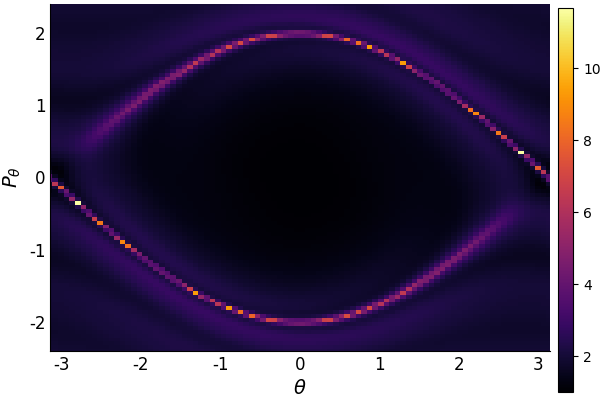
\includegraphics[width = \textwidth]{seprate_max_scalar_pendulum}
	\caption{Campo escalar $\zeta_+(\xo)$.}
	\label{fig:seprate_max_scalar_pendulum}
\end{subfigure}
%
\begin{subfigure}{0.49\textwidth}
	\centering
	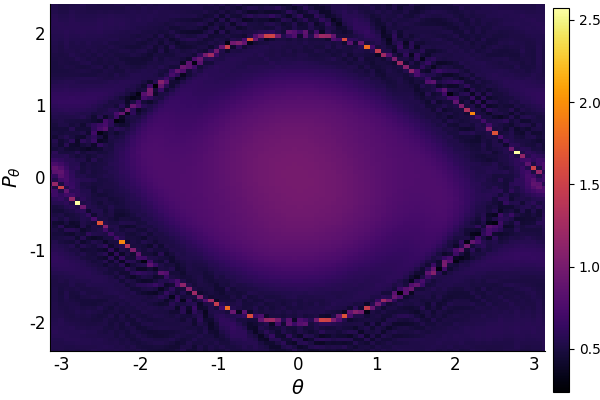
\includegraphics[width = \textwidth]{seprate_min_scalar_pendulum}
	\caption{Campo escalar $\zeta_-(\xo)$.}
	\label{fig:seprate_min_scalar_pendulum}
\end{subfigure}
\caption{ Campos escalares $\left( \zeta_\pm(\xo) \right)^{1/3}$ para el péndulo simple, en rejillas de $90\times 90$, con tolerancia $\epsilon_{Taylor} = 10^{-20}$, orden de los jets $M=3$ y orden de la expansión $N=25$. }
\label{fig:seprate_scalar_pendulum}
\end{figure}

%Teniendo xi_max se puede ver en qué dirección se expande más (menos) la deformación de de dx. ESte se hace encontrando el máximo y mínimo en la vecindad evaluada. ¿Cómo serviría esto? 

\subsection{Formas Simplécticas}
\label{sec:formas-simplecticas}
%Motivar un poco porqué hablaríamos de formas simpléticas y decir que el desarrollo viene motivado del chaosbook... si se puede encontrar algún otro libro para complementar estaría muy bien. 

Consideremos la siguiente función
\begin{align*}
H: \mathcal{M} \subset \mathbb{R}^d\times\mathbb{R}^d &\to \mathbb{R} \\ 
	(\mathbf{q},\mathbf{p}) &\to H(\mathbf{q},\mathbf{p})
\end{align*}

que define al hamiltoniano, cuyas ecuaciones de movimiento son

\begin{align*}
 \dot{\mathbf{q}} &= \ \pder{H}{\mathbf{p}} \\
 \dot{\mathbf{p}} &= - \pder{H}{\mathbf{q}}. 
\end{align*}

Si definimos $\mathbf{x} := (\mathbf{q},\mathbf{p}) = (x_1,\ldots,x_{2d})^T$, entonces
\begin{equation}
 \dot{x_i} = \omega_{i,j} \pder{H(\mathbf{x})}{x_j}
 \label{eq:symplectic_ham_ode}
\end{equation}

donde
\begin{equation}
 \omega = 
    \begin{bmatrix}
    \mathbf{0} & \mathbf{I} \\
    -\mathbf{I} & \mathbf{0}
  \end{bmatrix}
 \label{eq:symplectic_omega}
\end{equation}

es una matriz de $2d\times 2d$, $\mathbf{0}$ es una matriz de ceros de $d\times d$ e $\mathbf{I}$ es la matriz identidad de $d\times d$. Notemos que (\ref{eq:symplectic_omega}) cumple
\begin{align}
 \omega^2 &= -\mathbf{I}  \nonumber \\
 \omega^T &= -\omega
 \label{eq:omega_properties}
\end{align}
para cualquier $d$.

\begin{definicion}
Sea $\omega$ una matriz que cumple las propiedades (\ref{eq:omega_properties}). Se dice que una matriz $g$ es \textbf{simpléctica} si
\begin{equation}
 g^T \omega g = \omega.
 \label{eq:symplectic_condition}
\end{equation}
%Ver lo de las formas bilineales... Posiblemente se pueda partir de una definición más formal/general y concluir esto para g. 
\end{definicion}

Las matrices que cumplen la definición anterior forman un \textbf{grupo simpléctico} denotado $Sd(d)$, que son un caso particular de los grupos de Lie.

Los \textbf{grupos de Lie} son grupos cuyos elementos dependen de un número finito de parámetros, i.e., $g = g(\eta) = g(\eta_1,\ldots,\eta_N)$. Dicho esto, y como se menciona en \cite{CBHamiltonianDynamics}, para los cálculos se suele escoger una base para operar dichas matrices y, para transformaciones infinitesimales del espacio fase, éstas toman la forma
\begin{equation}
 g(\delta \eta) := \mathbf{1} + \delta \eta \mathbf{T}
 \label{eq:symp_infinit_rotation}
\end{equation}

con $\lbrace T_1, \ldots, T_N \rbrace$ un conjunto de rotaciones\footnote{Dichas rotaciones representan las deformaciones infinitesimales de las transformaciones de $g$.} sobre el espacio fase.

Notemos que si al grupo de rotaciones (\ref{eq:symp_infinit_rotation}) le imponemos la condición (\ref{eq:symplectic_condition}) de simplecticidad

\begin{align*}
  \left( \mathbf{1} + \delta \eta \mathbf{T} \right)^T \omega \left( \mathbf{1} + \delta \eta \mathbf{T} \right) = \omega \implies 
  \cancel{\omega} + (\delta \eta \mathbf{T})^T \omega + \omega \delta \eta \mathbf{T} + \cancelto{\mathcal{O}(\norm{\delta \eta \mathbf{T}}^2)} {(\delta \eta \mathbf{T})^T \omega \delta \eta \mathbf{T}} = \cancel{\omega}  
\end{align*}

obtenemos una forma explícita para que éste sea simpléctico
\begin{equation}
  (\delta \eta \mathbf{T})^T \omega + \omega \delta \eta \mathbf{T} = \mathbf{0}.
  \label{eq:eq:symplectic_condition2}
\end{equation}

En el caso de tener un hamiltoniano $H(\mathbf{x})$, basta darse cuenta que
\begin{itemize}
\item $H(\mathbf{x})$ es, al menos, $\mathcal{C}^2(\mathcal{M})$; esto es, $\frac{\partial^2 H}{\partial x_i \partial x_j} = \frac{\partial^2 H}{\partial x_j \partial x_i}$.

\item Los generadores de las transformaciones infinitesimales del sistema de EDO (\ref{eq:ode}) están dadas por $A_{i,j}(\mathbf{x}) := \pder{f_i(\mathbf{x})}{x_j}$. $A_{i,j}(\mathbf{x})$ son los elementos de matriz de $A(\mathbf{x})$, la cual se conoce como \textbf{matriz de estabilidad} del sistema.

\item La matriz de estabilidad puede representarse en términos de $\omega$ como $A(\mathbf{x}) = \omega \Xi(\mathbf{x})$, donde $\Xi(\mathbf{x}) = \left[ \frac{\partial^2 H(\mathbf{x})}{\partial x_i \partial x_j} \right]$ es el \textbf{hessiano}, o matriz de segundas derivadas, de $H$.

\item Como $H$ es $\mathcal{C}^2(\mathcal{M})$, entonces $\Xi$ es simétrica y, por tanto, $\Xi = \Xi^T$.
\end{itemize}

Con las observaciones anteriores podemos ver que
\begin{align*}
 A(\mathbf{x})^T \omega + \omega A(\mathbf{x}) = \Xi(\mathbf{x})^T \cancelto{\mathbf{I}}{\omega^T \omega} + \cancelto{-\mathbf{I}}{\omega \omega}\Xi(\mathbf{x}) = \Xi(\mathbf{x})^T - \Xi(\mathbf{x}) = 0.
\end{align*}

Así, cualquier sistema hamiltoniano es un sistema simpléctico y cumple
\begin{equation}
 A^T\omega + \omega A = 0
 \label{eq:symplectic_hamiltonian}
\end{equation}
%Meterlo como corolario o teorema? Chance es más elegante.

%Valdrá la pena hablar/demostrar que la simplecticidad implica la conservación de volumen? 

Regresemos, como siempre, al caso del péndulo simple. Sabemos, por (\ref{eq:pendulo-ham}), que es un sistema hamiltoniano y, por tanto, debe de cumplir (\ref{eq:symplectic_hamiltonian}). La matriz de estabilidad de éste\footnote{Se toma, sin pérdida de generalidad, $g = m = l = 1$.} está dada por
\begin{equation*}
  A_{pend}(\theta,p_\theta) =
  \begin{bmatrix}
    0             & 1 \\
    -\cos(\theta) & 0
  \end{bmatrix},
\end{equation*}

entonces

\begin{align*}
  A_{pend}^T \omega + \omega A_{pend} &=
  \begin{bmatrix}
    0 & -\cos(\theta) \\
    1 & 0
  \end{bmatrix}   
  \begin{bmatrix}
    0  & 1 \\
    -1 & 0
  \end{bmatrix} 
  +
  \begin{bmatrix}
    0  & 1 \\
    -1 & 0
  \end{bmatrix} 
  \begin{bmatrix}
    0             & 1 \\
    -\cos(\theta) & 0
  \end{bmatrix} \\
  &=
  \begin{bmatrix}
    \cos(\theta)  & 0 \\
    0             & 1
  \end{bmatrix}
  +
  \begin{bmatrix}
    -\cos(\theta)  & 0 \\
    0              & -1
  \end{bmatrix}
  = 0 
\end{align*}

probando ``a mano'', que es un sistema simpléctico. Sin embargo, la matriz de estabilidad también se calculó a mano, y ese es un proceso que la construcción polinomial del transporte de jets nos puede ahorrar. Dado que parametrizamos las vecindades de la condición inicial vía $\xo \to \xo + \xi = P_{0,\xo}(\xi)$, si evaluamos $P_{0,\xo}(\xi)$ en el campo vectorial $f$ obtendremos la parametrización de éste alrededor de $\xo$ y, como la evaluación es un vector de polinomios en $\xi$, se puede obtener la matriz de estabilidad, cuyos elementos son $A_{i,j}(\xi) = \pder{f_i(P_{0,\xo=(0,0)}(\xi))}{\xi_j}$.

Ahora, el problema de probar la simplecticidad de esta manera es que la expansión $P_{0,(0,0)}(\xi)$ es una expansión finita y no representa necesariamente a $f(\xi)$. Sin embargo, resulta ser que si un sistema es hamiltoniano, el correspondiente sistema dado por la expansión de sus funciones en series de Taylor hasta orden $M < \infty$ también lo es.

\begin{teorema}
Sea 
\begin{align*}
  H: \mathcal{M} \subset \mathbb{R} \times\mathbb{R} &\to \mathbb{R} \\ 
  (q,p) &\to H(q,p)
\end{align*}
una función escalar que define al sistema
\begin{align}
 \dot{q} &= \ \pder{H}{p} = f_1(q,p) \nonumber \\
 \dot{p} &= - \pder{H}{q} = f_2(q,p).
 \label{eq:theorem_ode}
\end{align}
Si $f_i$ es $\mathcal{C}^\omega(\mathcal{M}) \ \forall i$, entonces $\exists! \  \mathcal{H}: \mathcal{M} \to \mathbb{R}$ que define a
\begin{align*}
 \dot{q} &= \ \pder{\mathcal{H}}{p} = P_{f_1}^M(q,p) \\
 \dot{p} &= - \pder{\mathcal{H}}{q} = P_{f_2}^M(q,p)
\end{align*}
con $P_{f_i}^M(q,p)$ la expansión de Taylor de orden $M$ de $f_i$.
\footnote{El teorema es generalizable para $\mathcal{M} \subset \mathbb{R}^d \times \mathbb{R}^d$. La demostración queda como ejercicio para el lector.}
\end{teorema}

\begin{proof}
Como $f_i$ es $\mathcal{C}^\omega(\mathcal{M}) \ \forall i$, pueden expresarse como
\begin{align*}
 f_1(q,p) &= \sum_{i,j = 0}^\infty a_{i,j} q^i p^j \\
 f_2(q,p) &= \sum_{i,j = 0}^\infty b_{i,j} q^i p^j. 
\end{align*}
Así, por (\ref{eq:theorem_ode}), resolvemos $H(q,p)$ integrando
\begin{align*}
 H(q,p) &= \int f_1(q,p) dp = \sum_{i,j = 0}^\infty \frac{a_{i,j}}{j+1} q^i p^{j+1} + \ell_1(q) \\
 H(q,p) &= -\int f_2(q,p) dq = -\sum_{i,j = 0}^\infty \frac{b_{i,j}}{i+1} q^{i+1} p^j + \ell_2(p)
\end{align*}
encontrando la relación 
\begin{equation*}
 \frac{a_{i+1,j}}{j+1} = - \frac{b_{i,j+1}}{i+1} 
\end{equation*}
y la forma explícita de $\ell_i$
\begin{align*}
 \ell_1(q) &= \sum_{i=0}^\infty \frac{b_{i,0}}{i+1} q^i \\
 \ell_2(p) &= \sum_{i=0}^\infty -\frac{a_{0,i}}{i+1} p^i.
\end{align*}
Como todo lo anterior es cierto término a término, podemos truncar a cualquier orden $M < \infty$ y construir $\mathcal{H}$ con las expansiones truncas $P_{f_1}^M(q,p)$ y $P_{f_2}^M(q,p)$. \qed
\end{proof}

\begin{corolario}
Si $H$ define un sistema hamiltoniano, entonces $\mathcal{H}$ es simpléctico. 
\end{corolario}

Así, como sabemos que los ejemplos construidos hasta ahora vienen de un hamiltoniano $H(q,p)$, entonces la expansión polinomial $f(P_{0,(0,0)}(\xi))$ define una matriz de estabilidad simpléctica. 

Otra forma de ver la simplecticidad de un sistema es usando directamente (\ref{eq:symplectic_condition}) e interpretando la matriz $g$. Hay una visión geométrica que plantea Arnold \cite{Arnold1989} en su capítulo de variedades simplécticas, donde una estructura simplética es una 2-forma cerrada, lo cual representa la conservación del espacio fase. De este modo, la matriz $g$ se puede representar con el jacobiano de $\phi(t;t_0,\xo)$ y, para cualquier tiempo $t$ del flujo, un sistema es simpléctico cumple
\begin{equation}
 J(\phi(t))^T \omega J(\phi(t)) = \omega \ \forall t.
 \label{eq:sympletic_flow}
\end{equation} 
tal como se propone en la sección 42 de dicho capítulo del Arnold.

Esta forma de ver la simplecticidad es una mejor opción para ver qué tan buena es la integración de un sistema dado. Como el transporte de jets parametriza las vecindades de una trayectoria en el espacio fase, se puede obtener fácilmente el jacobinano para cada punto de ésta, y comprobar la simplecticidad de los sistemas se vuelve un proceso bastante directo una vez obtenida la solución. En este sentido, además de cualquier constante de movimiento que pueda tener un sistema, éste es un indicador de qué tan buena es la integración siempre que se tenga un sistema hamiltoniano.

%FIGURA! 
\begin{figure}[h!]
 \centering
 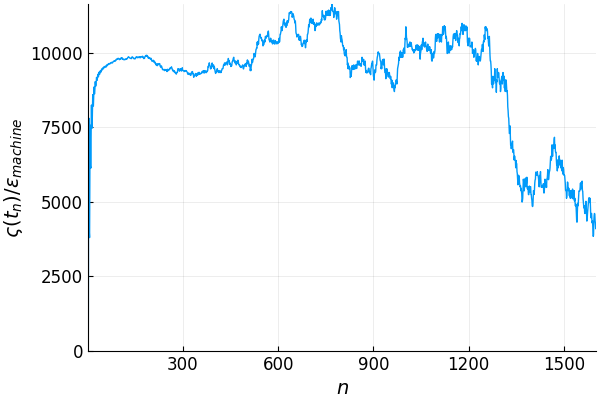
\includegraphics[width=0.8\linewidth]{simplecticity_pendulum}
 \caption{}
 \label{fig:simplecticity_pendulum}
\end{figure}

La figura \ref{fig:simplecticity_pendulum} muestra la variación de la cantidad $\varsigma(t)$ para el péndulo simple en términos de $\epsilon_{mahcine}$. Ésta se define como
\begin{equation}
 \varsigma(t) = \sum_{i,j} |\left[ J(\phi(t))^T \omega J(\phi(t)) - \omega \right]_{i,j}|
 \label{eq:scalar_symplecticity}
\end{equation}
y no es más que la suma de los valores absolutos de los elementos de matriz de (\ref{eq:sympletic_flow}). $\varsigma$ es una forma escalar de representar la simplecticidad del sistema para poder visualizarlo gráficamente para cada paso temporal.
  
Podemos observar en dicha figura un comportamiento browniano, similar a como pasa con la energía en los ejemplos de sistemas hamiltonianos planteados hasta ahora.


\subsection{Parametrización de parámetros}
\label{sec:parameter_variation}
Aunque el título de esta sección suene redundante, el TJ nos permite no sólo parametrizar las vecindades de $\xo$ en un campo vectorial dado sino también los parámetros que lo definen.

Tomemos, por ejemplo, al oscilador armónico\footnote{Al pobre oscilador armónico le deben picar las orejas de tanto que hablamos de él.} dado por  
\begin{equation}
 \ddot{x}(t) + \omega^2 x(t) = 0
 \label{eq:one_dim_oscil}
\end{equation}

cuyo hamiltoniano está dado por 
\begin{equation}
 H(x,y) = \frac{1}{2} \left( y^2 + \omega ^2 x^2 \right),
 \label{eq:osc_ham2}
\end{equation}
con $y = \dot{x}$.

Complejificando el dominio, sabemos que la solución está dada por 
\begin{equation*}
 x_{\mathbb{C}}(t) = A e^{i\omega t} + B e^{-i \omega t}
\end{equation*}
donde, si $\omega^2 < 0$, entonces la proyección a los reales es
\begin{equation}
 x(t) = a \cos(t) + b \sin (t)
 \label{eq:ho_solution_trig}
\end{equation}
y, si $\omega^2 > 0$, la proyección es
\begin{equation}
 x(t) = \alpha e^{\omega t} + \beta e^{- \omega t}.
 \label{eq:ho_solution_exp}
\end{equation}

%FIGURA!
\begin{figure}[h!]
 \centering
 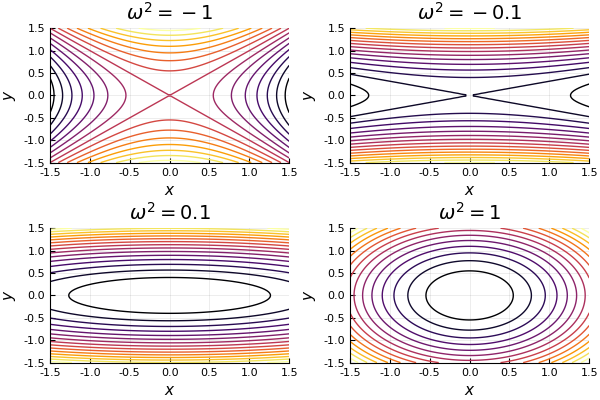
\includegraphics[width=0.8\linewidth]{oscillator_domega}
 \caption{Curvas de nivel dadas por (\ref{eq:osc_ham2}) para diferentes valores de $\omega^2$.}
 \label{fig:oscillator_domega}
\end{figure}

Observamos en la figura \ref{fig:oscillator_domega} cómo las curvas de nivel cambian para distintas $\omega^2$; en particular, observamos que las soluciones cambian de topología cuando $\omega^2$ cambia de signo. Con esto, pensar en una \textit{parametrización del parámetro} resulta una herramienta poderosa en el estudio de este tipo de sistemas ya que, por un lado, puede funcionar como un indicador para cambios de topología y, por otro, ayudar a encontrar conjuntos de soluciones cuando los parámetros no se conocen con exactitud. 

Para hacer esto con el transporte de jets, basta con incluir al parámetro o los parámetros que se quieran variar en el sistema de ecuaciones como $\dot{\lambda} = 0$, donde $\lambda$ es el conjunto de parámetros que se quieren variar. En este ejemplo el sistema queda como
\begin{align*}
 \dot{x} &= y \\
 \dot{y} &= - \omega^2 x \\
 \dot{\omega^2} &= 0
\end{align*}.
 
%FIGURA! 
\begin{figure}[h!]
 \centering 
 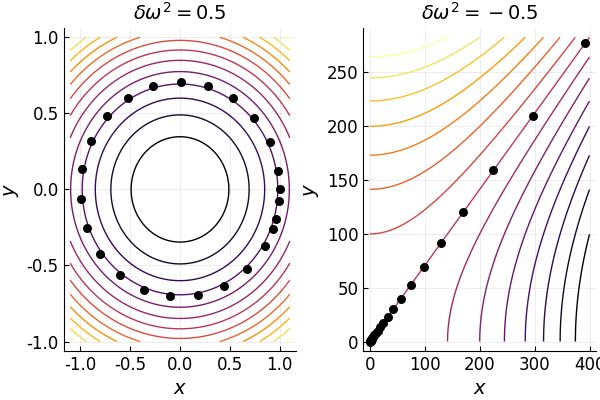
\includegraphics[width=0.8\linewidth]{oscillator_domega2}
 \caption{Solución para condición inicial $\xo = (1,0,0)$ y variación del parámetro para $\delta \omega^2 = 0.5$ en la izquierda y $-0.5$ en la derecha. $\delta \omega$ es un polinomio de orden $30$, y la expansión de Taylor para la solución es de orden $28$, con tolerancia de $10^{-20}$. Son $25$ pasos de integración de $0$ a $2 \pi$.}
 \label{fig:oscillator_param_transport}
\end{figure}

La figura \ref{fig:oscillator_param_transport} muestra el trasnporte de jets para $\omega^2$ para la condición inicial $\omega^2 = \omega_0^2 + \delta \xi$. En este caso $\omega_0^2 = 0$ y $\delta\xi = \pm 0.5$. Resulta que el transporte de jets sí obtiene el cambio de topología dado por el signo de $\omega^2$. Sin embargo, hay que ver qué tan precisa es la solución, lo cual se puede checar con la conservación de la energía al evaluar el hamiltoniano. 

El flujo conserva la energía cada vez menos conforme pasa el tiempo como se observa en la figura \ref{fig:oscillator_dE_domega}; de hecho, la solución que diverge más pierde hasta $15000$ epsilons casi al final de la integración. Sin embargo, el error máximo en términos absolutos es de $3.63 \times 10^{-12}$, lo cual es bastante aceptable.

%FIGURA! 
\begin{figure}[h!]
 \centering
 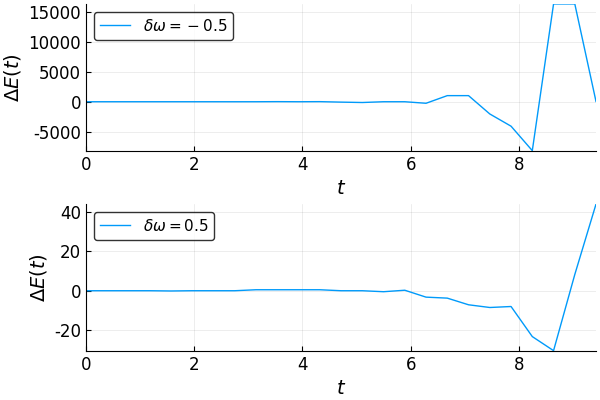
\includegraphics[width=0.8\linewidth]{oscillator_dE_domega}
 \caption{Variación $\Delta E = \frac{1}{\epsilon_{machine}} \left( E(t) - E_0 \right)$ de la energía respecto a la condición inicial para ambas evaluaciones del transporte $\delta \omega < 0$ y $\delta \omega > 0$.}
 \label{fig:oscillator_dE_domega}
\end{figure}


%Pequeña conclusión de sección ? 

%% Para que de nuevo haya salto de linea. (buscar Dutch style)
\setlength{\parskip}{1.3ex plus 0.2ex minus 0.2ex}

\chapter{Problema Restringido de Tres Cuerpos} 
\label{chap:CR3BP}
%%Relacionar mejor el inicio de este capítulo en relación a lo escrito en la introducción. Lo de ahorita es, en principio, preliminar. 

El objetivo de esta tesis es sacarle todo el provecho posible al transporte de jets y los indicadores que éste nos pueda regalar. Por esto, dos problemas físicos sencillos pero interesantes serán desarrollados en esta sección. El primero es el \textit{problema restringido de 3 cuerpos en una órbita circular (PR3COC)} y el segundo el \textit{sistema de Henón-Heiles (SHH)}. Antes de entrarle de lleno a estos problemas, creo que vale la pena recapitular un poco sobre la teoría en la que están basados; la mecánica analítica. Este capítulo se desarrollará como sigue: primero se hará un repaso de la mecánica lagrangiana y hamiltoniana muy al estilo de Landau y Lifshitz, específicamente en los capítulos I,II y VII de \cite{mechanics_landau_lifshitz}, luego, se desarrollará la teoría de PR3COC y, finalmente la de SHH.

\section{Problema de tres cuerpos sin restricciones}
\label{sec:3BP}

El problema de tres cuerpos interactuando en campos gravitacionales ha sido uno de gran controversia desde hace más de 300 años ya que la dinámica de éste tiene comportamientos que distan de ser obvios. Aún en el caso más simplificado, o sea, el caso restringido de tres cuerpos en órbitas circulares (PR3COC), el problema presenta alta sensibilidad a las condiciones iniciales, varios puntos de equilibrio, órbitas periódicas y semiperiódicas y, en general, una rica dinámica. Además,el PR3COC tiene únicamente dos grados de libertad (en vez de los 18 del problema general de tres cuerpos) lo cuál permite un estudio y una representación gráfica mucho más alcanzable respecto al problema original. En este sentido, se antoja analizar dicha dinámica con las herramientas desarrolladas en \ref{chap:jt_indicators}.

Adicionalmente, el apéndice \ref{chap:mecanics} tiene un repaso general de la mecánica analítica, de la cual se basa el plantemiento de este problema. 

El problema es planteado con el potencial gravitacional de Newton entre pares de cuerpos 
\begin{align}
 U_{M_1}(\mathbf{r}_1,\mathbf{r}_2,\mathbf{r}_3) &= -G \frac{M_1 M_2}{r_{1,2}} - G \frac{M_1 M_3}{r_{1,3}} \\
 U_{M_2}(\mathbf{r}_1,\mathbf{r}_2,\mathbf{r}_3) &= -G \frac{M_2 M_1}{r_{2,1}} - G \frac{M_2 M_3}{r_{2,3}} \\
 U_{M_3}(\mathbf{r}_1,\mathbf{r}_2,\mathbf{r}_3) &= -G \frac{M_3 M_1}{r_{3,1}} - G \frac{M_3 M_2}{r_{3,2}}
 \label{eq:3body_potential}
\end{align}

con $G$ la constante de gravitación universal, $\mathbf{r}_i = x_i \hat{\imath} + y_i \hat{\jmath} + z_i \hat{k}$ la posición de la i-ésima partícula, $M_i$ su masa y $r_{i,j} = \norm{ \mathbf{r}_i - \mathbf{r}_j}$ la distancia entre las partículas $M_i$ y $M_j$\footnote{Notemos la simetría $r_{i,j} = r_{j,i}$, aunque $\mathbf{r}_{i,j} = \mathbf{r}_i - \mathbf{r}_j = \mathbf{r}_j - \mathbf{r}_i  = - \mathbf{r}_{j,i}$.}. 

La energía cinética del problema la definimos de la manera usual 
\begin{equation}
 T(\dot{\mathbf{r}}_1,\dot{\mathbf{r}}_2,\dot{\mathbf{r}}_3) = \sum_{i=1}^3 M_i \dot{r}_i^2,
 \label{eq:3body_cinetic}
\end{equation}
lo cual define un sistema de 6 ecuaciones de movimiento dadas por (\ref{eq:newton_second_law})
\begin{equation}
 M_i \ddot{\mathbf{r}_1,\mathbf{r}_2,\mathbf{r}_3} = - G M_i \sum_{j\neq i} \frac{M_j}{r_{i,j}^2} \hat{\mathbf{r}}_{i,j},
 \label{eq:3body_eqs_motion}
\end{equation}
con $\hat{\mathbf{r}}_{i,j} = \frac{\mathbf{r}_{i,j}}{r_{i,j}}$ un vector unitario en la dirección de $\mathbf{r}_{i,j}$.

Éste es el caso más general del problema de tres cuerpos ya que ninguna restricción ha sido impuesta hasta el momento. Sin embargo, para el problema \textbf{restringido} de tres cuerpos uno supone que una de las partículas tiene una masa tan baja que no afecta a las otras dos y, por esto, las dos más grandes se mueven como si la tercera no existiera. Vale la pena estudiar primero el caso de dos cuerpos, ver la dinámica entre las dos partículas más masivas y luego regresar a estudiar el movimiento de la tercer partícula bajo la influencia de estas dos. 

\section{Problema de dos cuerpos}
\label{sec:2body_problem}
Dadas que $M_1$ y $M_2$ son los cuerpos de mayor masa o \textit{primarios} y $m_3$ es despreciable, la dinámica de dichos cuerpos primarios queda definida por
\begin{equation}
 \mathbf{F}_1(\mathbf{r}_1,\mathbf{r}_2) = M_1 \ddot{\mathbf{r}}_1 = -G \frac{M_1 M_2}{r_{1,2}^2} \hat{\mathbf{r}}_{1,2}.
 \label{eq:2body_eqs_motion}
\end{equation}
Como $\hat{\mathbf{r}}_{1,2} = - \hat{\mathbf{r}}_{2,1}$ entonces $\mathbf{F}_2 = -\mathbf{F}_1$, lo cual es equivalente a la tercera ley de Newton. Se tomará como referencia el desarrollo de \cite{} para obtener las soluciones de este problema. Por comodidad llamaremos a $\mathbf{r}_{1,2}$ simplemente $\mathbf{R}$ y, en términos de ésta, se puede plantear el \textit{problema de Kepler}, que describe la aceleración relativa
\begin{equation}
 \ddot{\mathbf{R}} = \ddot{\mathbf{r}}_1 - \ddot{\mathbf{r}}_2 = -G \frac{M_1 + M_2}{R^2} \hat{\mathbf{R}} = - \frac{\beta}{R^2}\hat{\mathbf{R}}
 \label{eq:kepler_problem}
\end{equation}
con $\beta = G \left(M_1 + M_2 \right)$. Multiplicando (\ref{eq:kepler_problem}) por $\mu := \frac{M_1 M_2}{M_1+M_2}$ obtenemos las ecuaciones de movimiento de la fuerza relativa de $M_1$ respecto a $M_2$ como si $M_2$ estuviera fija y $M_1$ tuviera la \textit{masa reducida} $\mu$.

El problema de Kepler conserva el momento angular $\mathbf{L} := \mathbf{R} \times \mathbf{p}$, ya que
\begin{equation}
 \frac{d\mathbf{L}}{dt} = \frac{d}{dt}\left(\mathbf{R} \times \mu\dot{\mathbf{R}} \right) = \mu\dot{\mathbf{R}} \cancelto{0}{\times}\dot{\mathbf{R}} + \mathbf{R} \times \mu \ddot{\mathbf{R}} = - \mathbf{R} \cancelto{0}{\times} G\frac{\mu \beta}{r^2}\hat{\mathbf{R}} = 0
\end{equation}
y, por tanto, $\mathbf{L} = \text{constante}$. Como primera consecuencia $\mathbf{R}$ y $\dot{\mathbf{R}}$ son perpendiculares a $\mathbf{L}$ y por tanto, viven en un plano. Por comodidad se escogerá un eje coordenado tal que dicho plano esté sobre $xy$. 

Una mejor descripción del movimiento se puede obtener en coordenadas polares, donde
\begin{align}
 \hat{R} &= \cos \theta \hat{\imath} + \sin \theta \hat{\jmath} \nonumber \\
 \hat{\theta} &= -\sin \theta \hat{\imath} + \cos \theta \hat{\jmath}
 \label{eq:polar_transformation}
\end{align}
y $z$ ya no necesita descripción ya que $z=0$ para toda la trayectoria. 

Debemos encontrar ahora las expresiones de $\mathbf{R}$,$\dot{\mathbf{R}}$ y $\ddot{\mathbf{R}}$ para replantear las ecuaciones de movimiento del sistema. Haciendo regla de la cadena obtenemos
\begin{align}
 \mathbf{R} &= R \cos \theta \hat{\imath} + R \sin \theta \hat{\jmath} = R \hat{R} \\
 \dot{\mathbf{R}} &= \left( \dot{R} \cos \theta - R \sin \theta \dot{\theta} \right) \hat{\imath} + \left( \dot{R} \sin \theta + R \cos \theta \dot{\theta} \right) \hat{\jmath} = \dot{R}\hat{R} + R \dot{\theta} \hat{\theta} \\
 \ddot{\mathbf{R}} &= \left(\ddot{R} - R \dot{\theta}^2 \right) \hat{R} + \left( R \ddot{\theta} + 2 \dot{R}\dot{\theta} \right) \hat{\theta}.
 \label{eq:motion_polar_variables}
\end{align}

De hecho, en éste sistema de coordenadas es fácil ver que
\begin{equation}
 L = \norm{ \mathbf{L} } = \norm{ \mathbf{R} \times \mu \dot{\mathbf{R}} } = \norm{ \left( R \hat{R} + 0 \hat{\theta} + 0 \hat{k} \right) \times \left( \dot{R} \hat{R} + R \dot{\theta} \hat{\theta} + 0\hat{k} \right) } = \mu R^2 \dot{\theta}
\end{equation}
para encontrar una expresión para la velocidad angular 
\begin{equation}
\dot{\theta}(R) = \frac{L}{\mu R^2}.
\label{eq:2body_ang_vel}
\end{equation}

Ahora, con (\ref{eq:motion_polar_variables}) podemos replantear (\ref{eq:kepler_problem}) y obtener las ecuaciones de movimiento en las nuevas coordenadas
\begin{align}
 R \ddot{\theta} + 2 \dot{R} \dot{\theta} &= 0 \\
 \ddot{R} - R \dot{\theta}^2 &= -\frac{\beta}{R^2}.
 \label{eq:2body_eqs_motion_polar}
\end{align}
Notemos que la primera queda resuelta por (\ref{eq:2body_ang_vel}) mientras que la segunda, notando la relación $\dot{R} = \frac{d R}{d\theta} \dot{\theta}$, se convierte en
\begin{align*}
 \frac{d^2 R}{d \theta^2} \dot{\theta}^2 + \frac{dR}{d\theta} \ddot{\theta} - R \dot{\theta}^2 = - \frac{\beta}{R^2}
\end{align*}
donde 
\begin{equation*}
 \ddot{\theta} = -\frac{2L}{\mu R^3}\dot{R} = -\frac{2L}{\mu R^3} \frac{dR}{d\theta}\dot{\theta} = - \frac{2L^2}{\mu^2 R^5} \frac{dR}{d\theta}.
\end{equation*}
Ésto y (\ref{eq:2body_ang_vel}) se sustituyen en  (\ref{eq:2body_eqs_motion_polar}) para obtener
\begin{equation*}
 \frac{L^2}{\mu^2 R^4}\left( \frac{d^2R}{d\theta^2} - \frac{1}{R} \left(\frac{dR}{d\theta} \right)^2 -R \right) = - \frac{\beta}{R^2}.
\end{equation*}

Finalmente, si hacemos $u(R) := \frac{1}{R}$, se simplifica la ecuación diferencial a
\begin{equation}
 \frac{d^2u}{d\theta^2} + u = \frac{\beta \mu^2}{L^2},
\end{equation}

que no es más que un oscilador armónico con forzamiento constante $\frac{\beta \mu^2}{L^2}$. Obtenemos explícitamente la solución para $u$:

\begin{equation*}
 u(\theta) = \frac{\beta \mu^2}{L^2} \left( 1 + e \cos (\theta - \theta_0 ) \right) 
\end{equation*}
\begin{equation}
 \therefore R(\theta) = \frac{L^2}{\beta \mu^2 \left(1 + e \cos (\theta - \theta_0) \right)}.
 \label{eq:2body_solution}
\end{equation}

%Cómo obtenemos explícitamente la forma de $e$ y de $\theta_0$? 
%Por qué esta ecuación representa una sección cónica en polares? Debería simplemente decirlo y citar algún texto? Chance sí...  

Ésta es la distancia relativa que tienen $M_1$ y $M_2$ en función del ángulo $\theta$. Notemos que (\ref{eq:2body_solution}) representa diferentes secciones cónicas en coordenadas polares y depende de la eccentricidad $e$ que tenga. 

\section{Problema restringido de 3 cuerpos en una órbita circular (PR3COC)}

Es ahora que estamos en posición de empezar a poner constricciones al problema de los tres cuerpos. 

Como ya se había mencionado, supondremos que la tercer partícula será mucho más pequeña que las otras dos, i.e., $m_3 \ll M_2 \leq M_1$. Así, la suposición principal es que $m_3$ no afecta la dinámica de $M_2$ ni de $M_1$ y, por tanto, la solución para $U_{M_1}$ y $U_{M_2}$ es la de los dos cuerpos desarrollada en \ref{sec:2body_problem}. En este sentido sólo queda por estudiar el comportamiento de $m_3$ en influencia de los cuerpos primarios.

Para restringir las órbitas a que sean circulares es necesario imponer que $R(\theta)$ tenga eccentricidad $e=0$; la cual queda de la forma
\begin{equation}
 R = \frac{L^2}{\mu^2 \beta}.
 \label{eq:3body_restricted_solution}
\end{equation} 

Con esto podemos dar una expresión para la velocidad angular que no dependa del momento angular $L$, es decir, con (\ref{eq:3body_restricted_solution}) en (\ref{eq:2body_ang_vel}) se obtiene
\begin{equation}
 \Omega := \dot{\theta} = \sqrt{ \frac{\beta R}{R^4} } = \sqrt{\frac{G \left(M_1 + M_2 \right)}{R^3}},
 \label{eq:3body_ang_velocity}
\end{equation}
que sólo depende de la distancia entre los cuerpos más masivos y la masa de cada uno de ellos. Notemos que al estar restringido el movimiento a órbitas circulares $R$ es constante en todo momento y por ello la velocidad angular también.

Para trabajar la dinámica de $m_3$ conviene establecer un marco de referencia en rotación de modo que $M_1$ y $M_2$ estén en reposo. Dicha rotación tendrá velocidad angular $\Omega$ y estará basada en el centro de gravedad entre las dos. Recordemos, de la sección \ref{sec:ficticious_forces}, que un sistema de referencia en rotación traerá algunas fuerzas ficticias descritas por (\ref{eq:rotating_constant_acceleration}), más específicamente la aceleración de Coriolis y la aceleración centrípeta. Como en este caso el sistema está centrado en el centro de gravedad de $M_1$ y $M_2$, la aceleración inercial será nula en todo momento.

Las ecuaciones para $m_3$ en este sistema quedan descritas como
\begin{equation}
 \ddot{\mathbf{r}} + 2\mathbf{\Omega} \times \dot{\mathbf{r}} = - \nabla V(\mathbf{r})
 \label{eq:3body_restricted_acceleration}
\end{equation}
con $\mathbf{r} = (x,y,z)$ la distancia de $m_3$ al centro de gravedad, $\mathbf{R} = \mathbf{r}_1 - \mathbf{r}_2 = (r_1 + r_2,0,0)$ la distancia entre $M_1$ y $M_2$ y
\begin{equation}
 V(\mathbf{r}) = \left( -G \frac{M_1}{\sqrt{(x + r_1)^2 + y^2 + z^2}} - G \frac{M_2}{\sqrt{(x - r_2)^2 + y^2 + z^2}} - \frac{1}{2} \mathbf{\Omega}^2 \mathbf{r}^2 \right)
 \label{eq:3body_restricted_potential}
\end{equation} 
la parte cerrada del potencial, que se suele conocer como \textit{pseudo-potencial}, ya que si la velocidad es distinta de cero, la fuerza de Coriolis debe ser considerada para la dinámica de la partícula.
Existe una primera integral desl sistema si hacemos el producto interno de (\ref{eq:3body_restricted_acceleration}) por $\dot{\mathbf{r}}$, que resulta en 
\begin{align*}
 \ddot{x} \dot{x} + \ddot{y} \dot{y} &= \pder{V}{x}\dot{x} + \pder{V}{y} \dot{y} \\
 \implies \frac{1}{2} \left( \dot{x}^2 + \dot{y}^2 \right) &= \frac{d V}{dt} 
\end{align*}
\begin{equation}
 \therefore C_J = 2U - v^2,
 \label{eq:3body_jacobi_constant}
\end{equation}
donde a $C_J$ se le conoce como \textbf{constante de Jacobi}.

Aunque se pudo encontrar una primera integral al problema, hay que notar que éste no es conservativo, ya que la dinámica de la partícula depende explícitamente de la velocidad de ésta. $V$ se escribe de manera tal que las masas quedan alineadas con el eje $x$ y se mueven en el plano $z = 0$. De hecho, con afan de reducir aún más los grados de libertad, tomaremos condiciones iniciales para que $m_3$ viva siempre en este plano.

Así, las ecuaciones de movimiento se reducen a
\begin{align}
 \dot{x} &= v_x \\
 \dot{y} &= v_y \\
 \dot{v}_x &= \Omega^2 \left( x - \frac{ R^3 (1 - \alpha) (x+\alpha R) }{\left( (x+\alpha R)^2 + y^2 \right)^{3/2} } - \frac{ R^3 \alpha (x- (1 -\alpha) R) }{\left( (x - (1-\alpha) R)^2 + y^2 \right)^{3/2} } \right) + 2\Omega v_y \\ 
 \dot{v}_y &= \Omega^2 y \left( x - \frac{ R^3 (1 - \alpha) }{\left( (x+\alpha R)^2 + y^2 \right)^{3/2} } - \frac{ R^3 \alpha }{\left( (1 - (1-\alpha) R)^2 + y^2 \right)^{3/2} } \right) - 2\Omega v_x
\end{align}
donde
\begin{align*}
 \alpha :&= \frac{M_2}{M_1 + M_2} \\ 
 R_1 &= \alpha R \\
 R_2 &= (1 - \alpha) R.
\end{align*}

\subsection{Puntos lagrangianos}
\label{sec:lag_points}

Aún sin ser conservativo, vale la pena estudiar las curvas de nivel de pseudo-potencial ya que éste nos dará una buena intuición sobre cómo será la trayectoria de nuestra partícula. De hecho, los puntos singulares que puedan aparecer seguirán siéndolo cuando se tome en cuenta la aceleración de Coriolis. La figura \ref{fig:3body_pseudo_potential} presenta dichas curvas de nivel, donde se observan tres puntos singulares en el eje alineados a $M_1$ y $M_2$ que se suelen llamar $L_2$,$L_1$ y $L_3$, respectivamente. Otros dos puntos existen para $y \neq 0$ los cuales se conocen como $L_4$ y $L_5$. Éstos cinco reciben el nombre de \textit{puntos lagrangianos} en honor a los estudios de Joseph Lagrange sobre el tema.

%FIGURA! 
\begin{figure}[h!]
 \centering
 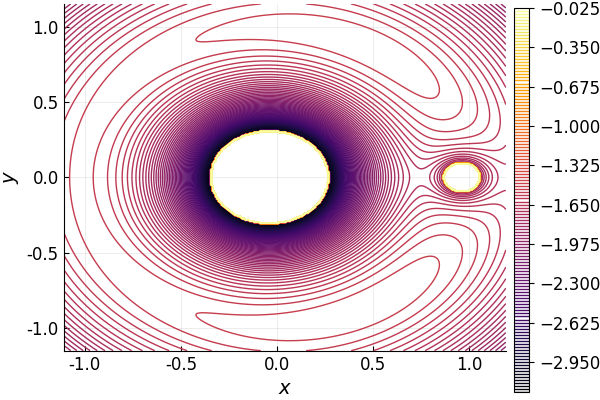
\includegraphics[width=0.8\linewidth]{pseudo_potential}
 \caption{Curvas de nivel para el pseudo-potencial $V(x,y)$ con $M_1 = 26M_2$, $R = 10$ Y $G=1$ en unidades adimensionales.}
 \label{fig:3body_pseudo_potential}
\end{figure}

Siguiendo el desarrollo de \cite{}, encontraremos dónde están dichos puntos singulares y se hará un análisis de estabilidad de éstos.

Los tres primeros se dan cuando $y=0$, quedando por resolver únicamente cuándo $\dot{v}_x = 0$. Esto plantea una ecuación de quinto grado en $x$ complicada de resolver analíticamente. Sin embargo, cuando $M_1$ es considerablemente más grande que $M_2$, se puede tomar la aproximación a primer orden de $\alpha$ y conseguir
\begin{align}
 L_1 &\approx \left( \left[ 1 - \left(\frac{\alpha}{3}\right)^{1/3} \right] R , 0 \right) \nonumber \\ 
 L_2 &\approx \left( R\left[ 1 + \left(\frac{\alpha}{3}\right)^{1/3} \right] R , 0 \right) \nonumber \\
 L_3 &\approx \left( -R\left[ 1 5 \frac{5 \alpha}{12} \right] R, 0 \right).
 \label{eq:3body_L123}
\end{align} 

También se pueden obtener estos valores numéricamente para cualquier $\alpha$, pero hace un poco más complicado el análisis de estabilidad ya que no se consiguen en función de $\alpha$ y $R$. Sin embargo, como se observa en la figura \ref{fig:3body_pseudo_xaxis}, para $\alpha = \frac{1}{27}$ sí se llega a notar la diferencia.

%FIGURA!
\begin{figure}[h!]
 \centering
 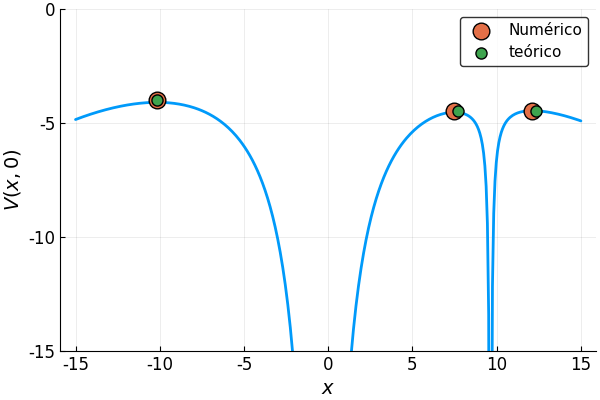
\includegraphics[width=0.8\linewidth]{pseudo_xaxis}
 \caption{Proyección del pseudo-potencial en el eje $x$ para ver sus puntos de inflexión. Aparecen $L_1, L_2$ y $L_3$ calculados con (\ref{eq:3body_L123}) (verde) y numéricamente (naranja).}
 \label{fig:3body_pseudo_xaxis}
\end{figure}

Para obtener $L_4$ y $L_5$ es importante destacar que la fuerza centrípeta es, por definición, radial hacia afuera. En este sentido, en la dirección radial se deben balancear la fuerza centrípeta con la gravitacional. Esto hace que el balance en la dirección tangencial sea debido únicamente a los dos objetos masivos interactuando bajo sus campos gravitacionales. Para obtener esto, hacemos una proyección de la fuerza hacia sus direcciones radiales y tangenciales con los vectores $\mathbf{r}_{\parallel} = (x,y)$ y $\mathbf{r}_{\bot} = (-y,x)$, así
\begin{align*}
 F_{\bot} &= \frac{1}{r_{\bot}} \mathbf{r}_{\bot} \cdot \mathbf{F} = \frac{\Omega^2R^3 y}{r_{\bot}} \left( - \frac{(1-\alpha)(x + \alpha R)}{ r_{1,3}^3 } - \frac{\alpha(x - (1-\alpha) R)}{ r_{2,3}^3 } + \frac{(1-\alpha)x}{ r_{1,3}^3 } + \frac{\alpha x}{ r_{2,3}^3 } \right) \\
 \therefore F_{\bot} &= \frac{\Omega^2R^3 \alpha (1-\alpha) y}{r_{\bot}} \left( \frac{1}{r_{1,3}^3} - \frac{1}{r_{2,3}^3} \right),
\end{align*}
es decir, la condición para que la componente tangencial de la fuerza se anule es que ambos cuerpos estén a la misma distancia de la partícula $m_3$, lo cual tiene sentido ya que el sistema tiene el origen en el centro de masa entre $M_1$ y $M_2$. 

Para la componente radial, tenemos que
\begin{align*}
 F_{\parallel} &= \frac{1}{r_{\parallel}} \mathbf{r}_{\parallel} \cdot \mathbf{F} = \frac{\Omega^2}{r_\parallel} \left( (x^2 + y^2) - R^3 (1-\alpha ) \left( \frac{(x+ \alpha R)x}{r_{1,3}^3} + \frac{y^2}{r_{1,3}^3} \right) - R^3 \alpha \left( \frac{(x - (1-\alpha) R)x}{r_{2,3}^3} + \frac{y^2}{r_{2,3}^3} \right) \right),
\end{align*}
pero $r_{1,3} = r_{2,3}$, por lo que lo anterior se simplifica a 
\begin{align*}
 F_{\parallel} = \frac{R^3 \Omega^2 (x^2 + y^2)}{r_\parallel} \left( \frac{1}{R^3} - \frac{1}{r_{1,3}^3} \right).
\end{align*}

Encontramos que $r_{1,3} = r_{2,3} = R$. $L_4$ y $L_5$ forman un tríangulo equilátero de lado $R$, cuya base es la distancia entre $M_1$ y $M_2$. Así,
\begin{align}
 L_4 &= \left( \frac{1 - 2\alpha}{2}  R , \frac{\sqrt{3}}{2} R \right) \\
 L_5 &= \left( \frac{1 - 2\alpha}{2}  R  , -\frac{\sqrt{3}}{2} R \right)
 \label{eq:L4_L5}
\end{align} 
tal como se ve en la figura \ref{fig:L_diagram}.

%FIGURA! 

%SI HACER EL ANALISIS DE LOS PUNTOS! YA QUE DE AQUI VIENE LA CONDICIÖN PARA QUE L4 Y L5 SEAN ESTABLES!
La estabilidad de estos puede estudiarse viendo cómo se comportan las ecuaciones de primera variación alrededor de los puntos de equilibrio, tal como se hace en \cite{WMAP}. Para esto basta construir la matriz de estabilidad 
\begin{equation*}
 A(\mathbf{x}) = \begin{bmatrix}
  \pder{\mathbf{f}_1}{x_1}(\mathbf{x}) & \dots & \pder{\mathbf{f}_1}{x_n}(\mathbf{x}) \\
  \vdots & \ddots & \vdots \\ 
  \pder{\mathbf{f}_n}{x_1}(\mathbf{x}) & \dots & \pder{\mathbf{f}_n}{x_n} (\mathbf{x})
\end{bmatrix}
\end{equation*}
donde $\dot{\mathbf{x}} = \mathbf{f}(\mathbf{x})$ y encontrar los eigenvalores de ésta para determinar qué tipo de punto singular se trata. Para éste caso
\begin{equation}
 A(\mathbf{x}_{L_i}) = \begin{bmatrix}
  0 & 0 & 1 & 0 \\
  0 & 0 & 0 & 1 \\ 
  \pder{\dot{v_x}(\mathbf{x}_{L_i})}{x} & \pder{\dot{v_x}(\mathbf{x}_{L_i})}{y} & 0 & 2 \Omega \\
  \pder{\dot{v_y}(\mathbf{x}_{L_i})}{x} & \pder{\dot{v_y}(\mathbf{x}_{L_i})}{y} & -2\Omega & 0
\end{bmatrix}
\end{equation}
representa dicha matriz, y ésta será evaluada en los puntos lagrangianos $\mathbf{x}_{L_i}$, donde 
\begin{align}
 \pder{\dot{v}_x}{x} &= \Omega^2 \left( 1 - R^3 \left( \frac{1-\alpha}{r_{1,3}^3} - 3\frac{(1-\alpha)(x + \alpha R)^2}{r_{1,3}^5} + \frac{\alpha}{r_{2,3}^3} - 3\frac{\alpha(x - (1-\alpha) R)^2}{r_{2,3}^5} \right) \right) \nonumber \\ 
 \pder{\dot{v}_y}{y} &= \Omega^2 \left( 1 - R^3 \left( \frac{1-\alpha}{r_{1,3}^3} - 3\frac{(1-\alpha)y^2}{r_{1,3}^5} + \frac{\alpha}{r_{2,3}^3} - 3\frac{\alpha y^2}{r_{2,3}^5} \right) \right) \nonumber \\
 \pder{\dot{v}_x}{y} &= \pder{\dot{v}_y}{x} = 3 \Omega^2 R^3 y \left( \frac{(1-\alpha )(x+\alpha R)}{r_{1,3}^5} + \frac{\alpha (x- (1-\alpha )R)}{r_{2,3}^5} \right),
 \label{eq:3body_stability}
\end{align}
con $r_{i,3}$ la distancia a $M_i$.

Para $L_1$, $L_2$ y $L_3$ se puede mostrar que son equilibrios inestables sin importar el valor de los cuerpos masivos ni la distancia entre ellas \cite{algo}. De hecho, sustituyendo para $L_1$ y $L_2$ se obtiene
\begin{align*}
 \lambda_\pm &= \pm \Omega \sqrt{1 + 2\sqrt{7}} \\
 \sigma_\pm &= \pm i \Omega \sqrt{2\sqrt{7} - 1}
\end{align*}
mientras que en $L_3$ obtenemos 
\begin{align*}
 \lambda_\pm &= \pm \Omega \sqrt{ \frac{3M_1}{8M_2} } \\
 \sigma_\pm &= \pm i \Omega \sqrt{7}
\end{align*}
donde $\lambda_\pm \in \mathbb{R}$ en ambos casos, lo cual representa sillas en el espacio de configuraciones.

Sustituyendo $L_4$ y $L_5$ en (\ref{eq:3body_stability}), se obtiene que $\pder{\dot{v}_x}{x} = \pm \frac{3}{4}\Omega^2$, $\pder{\dot{v}_y}{y} = \pm \frac{9}{4}\Omega^2$ y $\pder{\dot{v}_x}{y} = \pm \frac{3\sqrt{3}}{2} (1-2\alpha) \Omega^2$, cuyos eigenvalores son
\begin{align*}
 \lambda_\pm = \pm i \frac{\Omega}{2} \sqrt{ 2 - \sqrt{27(1-2\alpha)^2 - 23} } \\
 \sigma_\pm = \pm i \frac{\Omega}{2} \sqrt{ 2 + \sqrt{27(1-2\alpha)^2 - 23} } 
 \end{align*}

Estos puntos serán estables si sus eigenvalores son puramente imaginarios, cuya condición se cumple si 
\begin{align*}
 2 &\geq \sqrt{27(1-2\alpha)^2 - 23} \\
 23 &< 27(1-2\alpha)^2.
\end{align*}
Lo primero es equivalente a que 
\begin{equation}
 M_1 > \frac{1 + \sqrt{\frac{23}{27}} }{1 - \sqrt{\frac{23}{27}}}M_2 \approx 25M_2
\end{equation}
y lo segundo se da siempre que lo primero se cumple. 

Así, vemos explícitamente la condición para la estabilidad de los puntos $L_4$ y $L_5$. 

\subsection{Curvas de velocidad cero}
\label{sec:zvc}

Un último análisis que vale la pena hacer es aquel de las \textbf{curvas de velocidad cero} (CV0). Éstas son el punto máxmimo de retorno para una energía dada en el espacio de configuraciones. Podemos pensar, como analogía, que para una energía potencial dada, una partícula en caída libre no podrá rebotar más allá de cierta altura $h$ que dependa de dicha energía. De hecho, justo cuando la partícula alcance dicha altura, su velocidad será idénticamente cero y volverá a caer. 

Para encontrar estas curvas, se impone cierta pseudo-energía $C_J$ y se traza la curva tal que la velocidad sea cero, i.e.,
\begin{equation*}
 (x,y,0,0) = \left\lbrace V \ | \  V = \frac{1}{2}C_J \right\rbrace.
\end{equation*}

Como en el ejemplo de caída libre, todas las trayectorias estarán atrapadas ``debajo'' de esta curva y restringe las secciones en las que $m_3$ se puede mover. 

%FIGURA! 
\begin{figure}[h!]
 \centering
 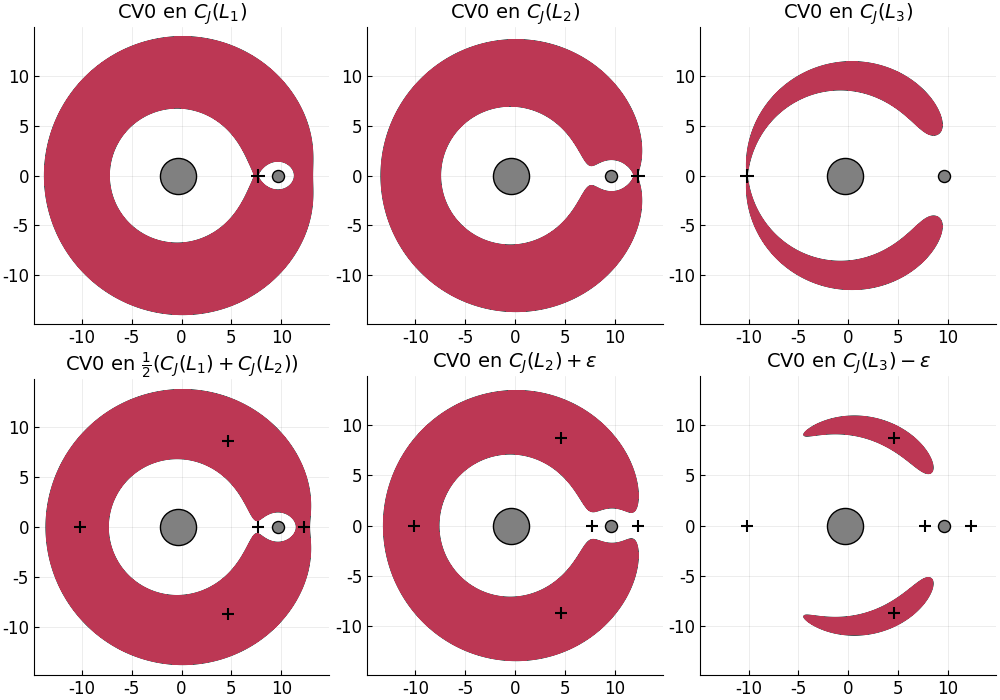
\includegraphics[width=0.9\linewidth]{zero_velocity_curves}
 \caption{\textit{Arriba:} curvas de velocidad cero (CV0) sobre los puntos $L_1, L_2$ y $L_3$, respectivamente. \textit{abajo:} CV0 sobre variaciones en energía sobre las de arriba, se tomó $\varepsilon = 0.05$.}
 \label{fig:zero_velocity_curves}
\end{figure}

La figura \ref{fig:zero_velocity_curves} muestra algunas de estas curvas con consantes de Jacobi alrededor de $L_1$, $L_2$ y $L_3$ y algunas variaciones respecto a estos\footnote{Se graficaron las energías mayores o iguales a la constante de Jacobi para ver la ``sección prohibida'' de las trayectorias.}. Al ser estos puntos tipo silla, dividen al espacio en regiones. El caso más interesantes está entre las energías de $L_1$ y $L_2$, ya que entre éstas se pueden diseñar condiciones iniciales que se queden siempre orbitando entre los dos planetas, o que se quede sólamente en uno de ellos eternamente.

%Falta escoger el segundo problema... esto será después de hacer todos los análisis pertinentes del CR3BP

% Para que de nuevo haya salto de linea. (buscar Dutch style)
\setlength{\parskip}{1.3ex plus 0.2ex minus 0.2ex}

\chapter{Resultados} 
\label{chap:results}
En el capítulo \ref{chap:CR3BP} se estudió el problema restringido circular de los tres cuerpos. Dos partículas primarias orbitando en un plano a velocidad constante respecto a su centro de masa y una tercera influenciada por las otras dos con una dinámica muy rica. Rica es por elementos como la sensibilidad al parámetro de masa, dada por la ecuación (\ref{eq:mu_critica}), la sensibilidad a condiciones inciales cercanas, las regiones discriminadas por su constante de Jacobi, o sus cinco puntos lagrangianos. Esta sección busca explotar el transporte de jets como se describe en el capítulo \ref{chap:jt} así como los indicadores y herramientas desarrolladas en \ref{chap:jt_indicators}.


Este capítulo se divide como sigue: La sección \ref{sec:parametrization} parametriza a $\mu$ y hace un TJ de dicha parametrización. La sección \ref{sec:asteroids} estudia la probabilidad de colisión entre dos asteroides orbitando cerca de la Tierra. Luego, en \ref{sec:C3BP_simplecticity} se estudia la simplecticidad del PC3C. Finalmente, en la sección \ref{sec:C3BP_heatmaps} se presentan los campos escalares y vectoriales de $\xi_{max}$ y $\theta_{\pm}$ y se compara con los resultados para el campo de ELTF.

\section{Parametrización de $\mu$}
\label{sec:parametrization}

Como se analizó en la sección \ref{sec:lag_points}, $L_i = L_i(\mu)$, es decir, los puntos de equilibrio del PC3C dependen todos del parámetro de masa del sistema. Los puntos $L_4(\mu)$ y $L_5(\mu)$ son de particular interés ya que, a diferencia de los otros tres, serán estables si $\mu \leq \mu_c$, donde $\mu_c$ es el parámetro crítico de la masa dado por (\ref{eq:mu_critica}). 

El análisis de eigenvalores alrededor de los puntos singulares nos da cómo es la estabilidad de dichos puntos. Sin embargo, es interesante ver las soluciones cerca de $\mu_c$ ya que nos permitirá ver directamente en el flujo el comportamiento de estabilidad de la partícula que visita a $L_4$ o $L_5$.

Para esto, se seguirá la filosofía de la sección \ref{sec:parameter_variation}, donde se agregará a las ecuaciones de movimiento la ecuación 
\begin{equation*}
 \dot{\mu} = 0.
\end{equation*}
Con esto, se hará un transporte en $\mu$, es decir, ésta se parametrizará como 
\begin{equation*}
 \mu = \mu_0 + \delta\mu,
\end{equation*}   
donde $\delta\mu \in \pkM$ y, por tanto, $\mu \in \pkM$ también. Se introduce la notación $\phi_\mu(t;t_0,\xo)$ para referirse a este tipo de transporte. Tomando $\mu_0 = \mu_c \approx 0.0385$, se está en el límite entre la estabilidad y la divergencia alrededor de los puntos $L_4$ y $L_5$.

%FIGURA!
\begin{figure}
 \centering
 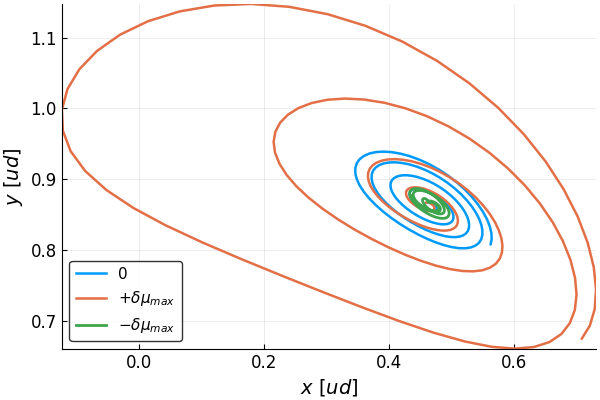
\includegraphics[width=0.8\linewidth]{flow_dmu}
 \caption{Espacio de configuraciones para $\phi_\mu$ con variaciones $\delta\mu = 0$ (azul), $\delta\mu = \delta\mu_{max}$ (naranja), y $\delta\mu = -\delta\mu_{max}$ (verde), donde $\delta\mu_{max} = \xi_{max}(\phi_\mu) \approx 0.00329$. Para el transporte se usó un jet de orden $M=18$ con condiciones iniciales $\left( L_{4_x}, L_{4_y} + \Delta y, 0, 0, \mu \right)$.}
 \label{fig:flow_dmu}
\end{figure}

Para el transporte, tomaremos como condición inicial a $\xo = \left( L_{4_x}, L_{4_y} + \Delta y, 0, 0, \mu \right)$ con $\Delta y = 7\times 10^{-4}$ para no estar exáctamente en el punto fijo. Las variaciones de $\delta\mu$ estarán acotadas por el tamaño máximo de vecindad de la expresión (\ref{eq:ximax}), es decir, $\lvert \delta\mu \rvert \leq \lvert \delta\mu_{max} \rvert = \xi_{max}(\phi_\mu) \approx 0.033$ en este caso. Se puede ver en la figura \ref{fig:flow_dmu} una integración a $40$ unidades temporales. Se observa cómo para $\delta \mu > 0$, las soluciones se alejan cada vez más de $L_4$, mientras que para $\delta \mu < 0$ se queda en cierta localidad. Una forma de observar este comportamiento de manera más clara es si medimos la separación de $\phi_\mu(t)$ respecto de $\xo$ para distintos valores de $\delta \mu$. La figura \ref{fig:remoteness_dmu} muestra esta separación en función del tiempo. Se puede observar que mientras mayor sea la variación de $\mu$, mayor es la tendencia y mayor la amplitud de oscilación. 

%FIGURA! 
\begin{figure}
 \centering
 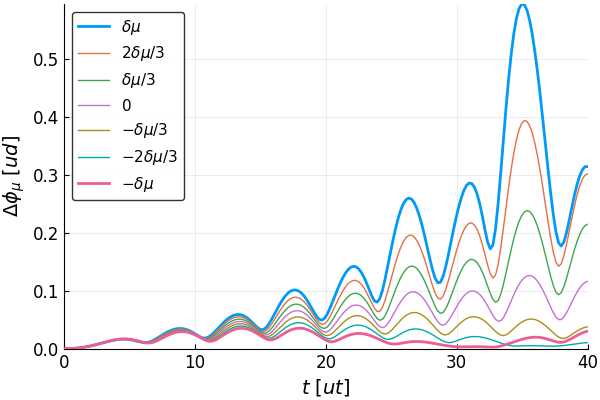
\includegraphics[width=0.8\linewidth]{remoteness_dmu}
 \caption{Diferencia $\Delta\phi_\mu(t) = \norm{ \phi_\mu(t) - \xo }$ del espacio de configuraciones para $\delta\mu \in \left\lbrace -\delta\mu_{max}, -2\delta\mu_{max}/3, -\delta\mu_{max}/3, 0, \delta\mu_{max}/3, 2\delta\mu_{max}/3, \delta\mu_{max}  \right\rbrace$.}
 \label{fig:remoteness_dmu}
\end{figure}

Una forma de ver realmente cuándo el flujo no diverge de la localidad de $L_4$ es si podemos aislar la tendencia de la amplitud de los ciclos. Para esto, se puede usar un filtro de Hodrick-Prescott, que separa una serie de tiempo en tendencia y ciclo. Sea $y_t$ la variable de una serie de tiempo al tiempo $t$. Se asume que dicha serie está compuesta de una componente de tendencia $\tau_t$ más una componente cíclica $c_t$, es decir, $y_t = \tau_t + c_t$\footnote{Normalmente se incluye una componente de error $\eta_t$ que, en este caso, será absorbida por $c_t$.}. Así, uno puede encontrar la tendencia, como se plantea en \cite{Hodrick1997}, bajo el problema de minimización
\begin{equation}
 \min_{\tau} \left( \sum_{t=1}^T (y_t - \tau_t)^2 + \lambda \sum_{t=2}^{T-1} \left[ (\tau_{t+1} - \tau_t) - (\tau_t - \tau_{t-1}) \right]^2 \right),
 \label{eq:hp-filter}
\end{equation} 
con $\lambda$ un parámetro positivo que regula la variabilidad en la componente de tendencia de la serie.

Tomaremos la solución matricial lineal de \cite{Kim2004}  
\begin{equation}
 \mathbf{y}_t = \left( \lambda \mathbf{F} + \mathbf{I}_t \right) \tau_t
 \label{eq:hp_matrix}
\end{equation}  
al derivar (\ref{eq:hp-filter}) respecto a $\tau_t$, donde
\begin{align}
 \mathbf{F} = \left[ \begin{array}{cccccccccc}
 1  & -2 & 1  & 0  & \cdots &        &        & & \cdots & 0    \\
 -2 & 5  & -4 & 1  & 0      & \cdots &        & & \cdots & 0    \\
 1  & -4 & 6  & -4 & 1      & 0      & \cdots & & \cdots & 0    \\
 0  & 1  & -4 & 6  & -4 & 1 & 0      & \cdots &        & \vdots \\
 \vdots  & \ddots  &  &  &  &  &  &  &        & \ddots          \\
    &    &    &  0 &  1 &-4 &    6   & -4     &      1 & 0      \\
   &   &  & \cdots &  0 & 1 &   -4   &  6     &      4 & 1      \\
   &   &  &  &   \cdots & 0 &    1   &  -4    &      5 & 2      \\
 0 &\cdots&  &  &  & \cdots &    0   &   1    &     -2 & 1      \\
 \end{array} \right],
\end{align}

ya que ésta es fácilmente programable. De (\ref{eq:hp_matrix}), obtenemos que $\mathbf{\tau}_t = \left( \lambda \mathbf{F} + \mathbf{I}_t \right)^{-1} y_t$ y $c_t = y_t - \tau_t$. Aplicando este filtro en la figura \ref{fig:remoteness_dmu}, se obtiene el ciclo y la tendencia tal como se presenta en la figura \ref{fig:trendcycle_dmu}. En ésta, se observa cómo desde la primera variación negativa ($\delta\mu = -\delta\mu_{max}/3$) hacia valores más negativos, la tendencia decrece después de llegar a un máximo. Esto quiere decir que la distancia respecto al punto inicial no diverge, como se había predicho en el análisis de estabilidad lineal de (\ref{eq:stability_CR3BP}). Por otro lado, es interesante ver cómo la amplitud de las oscilaciones en la parte cíclico de $\Delta\phi_\mu$ son mayores entre mayor sea $\delta_\mu$.

%FIGURA!
\begin{figure}[h!]
\centering
\begin{subfigure}{0.49\textwidth}
	\centering
	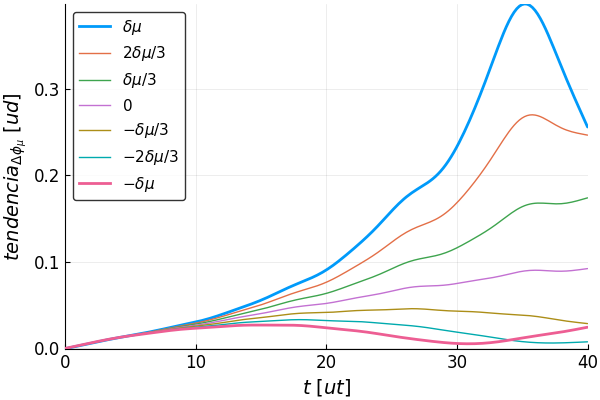
\includegraphics[width = \textwidth]{trends_dmu}
\end{subfigure}
%
\begin{subfigure}{0.49\textwidth}
	\centering
	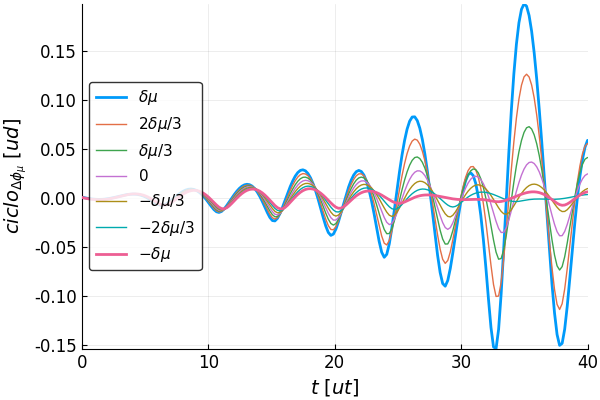
\includegraphics[width = \textwidth]{cycles_dmu}
\end{subfigure}
\caption{ Separación en tendencia (izquierda) y ciclo(derecha) de los valores de la figura \ref{fig:remoteness_dmu} usando un filtro de Hodrick-Prescott con $\lambda = 8000$.}
\label{fig:trendcycle_dmu}
\end{figure}

Hacer esta separación ayuda fuertemente al análisis de estabilidad de $\mu$ alrededor de $L_4$ y $L_5$ cuando $\mu = \mu_c \pm \delta\mu$, pero ¿seguirán siendo las órbitas en el caso donde $\mu \ll \mu_c$ como en el caso Tierra-Luna?

\subsection{Caso Tierra-Luna}
Dado que en la adimensionalización de las ecuaciones de movimiento el problema queda planteado únicamente en términos de $\mu$, basta ver que en el caso Tierra-Luna $M_T = 5.972 \times 10^{24} \textrm{kg} $, $M_L = 7.348 \times 10^{22} \textrm{kg}$ y, por tanto, $\mu_{TL} = 0.01215$. Notamos que $\mu_{TL} \ll \mu_c$ por lo que alrededor de $L_4$ y $L_5$ debería haber órbitas estables, aún cuando $\delta\mu_{max}$ sea grande.

%FIGURA!
\begin{figure}
 \centering
 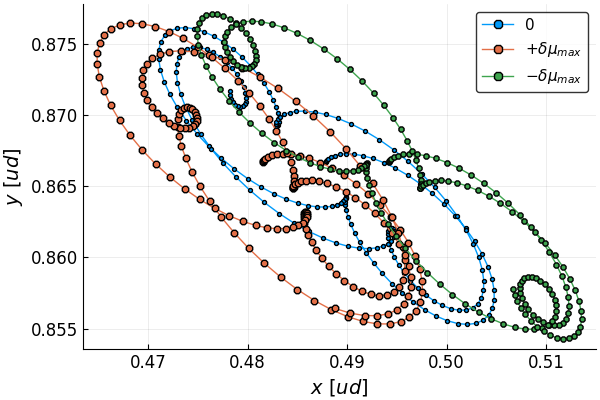
\includegraphics[width=0.8\linewidth]{flow_tl}
 \caption{Espacio de configuraciones para $\phi_\mu$ con variaciones $\delta\mu = 0$ (azul), $\delta\mu = \delta\mu_{max}$ (naranja), y $\delta\mu = -\delta\mu_{max}$ (verde), donde $\delta\mu_{max} = \xi_{max}(\phi_\mu) \approx 0.0063$. Para el transporte se usó un jet de orden $n=18$ con condiciones iniciales $\left( L_{4_x}, L_{4_y} + \Delta y, 0, 0, \mu \right)$.}
 \label{fig:flow_tl}
\end{figure}

Primero, al hacer el transporte de jets a $40$ unidades temporales y ver el espacio de configuraciones como se muestra en la figura \ref{fig:flow_tl}, se observa cómo las tres trayectorias $\delta\mu = \left\lbrace -\delta\mu_{max}, 0, \delta\mu_{max} \right\rbrace$ quedan siempre orbitando alrededor de $L_4$, es decir, no divergen. Resulta que $\delta\mu_{max} = 0.0063 $, lo cual equivale a una variación del $52.14 \%$ respecto a $\mu_{TL}$. Para ponerlo en perspectiva, $\mu_{TL}$ equivale a que la masa primaria (la Tierra) es unas $81$ veces más grande que la secundaria (luna). Así, $\mu_{TL} \pm \delta\mu_{max}$ equivale a que la masa primaria sea $53$ y $171$ veces más grande que la otra, respectivamente. Análogo a la figura \ref{fig:remoteness_dmu}, la figura \ref{fig:remoteness_tl} presenta la separación respecto a $\xo$ de la solución. Aquí se puede observar que, aunque al principio (en las primeras $8$ unidades, aproximadamente) las tendencias y oscilaciones siguen el mismo comportamiento que en el caso anterior, rápidamente se vuelven arbitrarias, sin tener tendencia aparente ni amplitudes creciente en los ciclos.

%FIGURA!
\begin{figure}
 \centering
 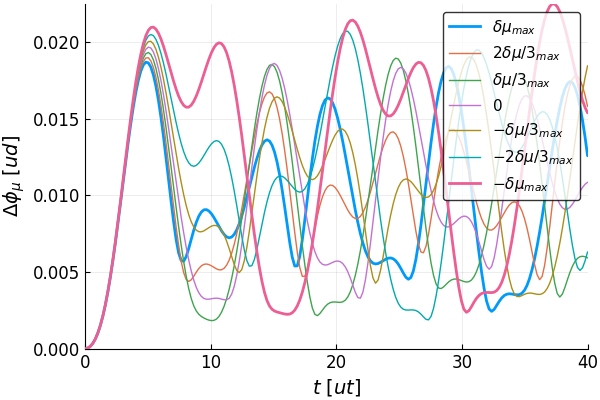
\includegraphics[width=0.8\linewidth]{remoteness_tl}
 \caption{Diferencia $\Delta\phi_\mu(t) = \norm{ \phi_\mu(t) - \xo }$ del espacio de configuraciones para $\delta\mu \in \left\lbrace -\delta\mu_{max}, -2\delta\mu_{max}/3, -\delta\mu_{max}/3, 0, \delta\mu_{max}/3, 2\delta\mu_{max}/3, \delta\mu_{max}  \right\rbrace$ integrado a $40$ unidades temporales.}
 \label{fig:remoteness_tl}
\end{figure}

De hecho, en la figura \ref{fig:trendcycle_tl} se muestran los gráficas al aplicar el filtro de Hodrick-Prescott. Al aplicar dicho filtro, ¡no se puede observar absolutamente nada! Ni la gráfica de ciclo ni la de tendencia tienen ninguna coherencia en realción a las variaciones del parámetro de masa. Esto significa que $\mu_{TL} + \delta\mu$ es, en efecto, estable para todo el conjunto de valores $\delta\mu$ evaluados alrededor de $L_4$ y $L_5$. Este es un caso donde el TJ es una herramienta natural para evaluar la estabilidad de estos puntos lagrangianos y para ver cómo varían las trayectorias en función de los parámetros del problema-. Muchas otras exploraciones se pueden hacer con variación de parámetros en el problema de tres cuerpos. Sin embargo, este análisis basta para ver las capacidades del TJ cuando no son específicamente ``Jets'' los que transporta.

%FIGURA!
\begin{figure}[h!]
\centering
\begin{subfigure}{0.49\textwidth}
	\centering
	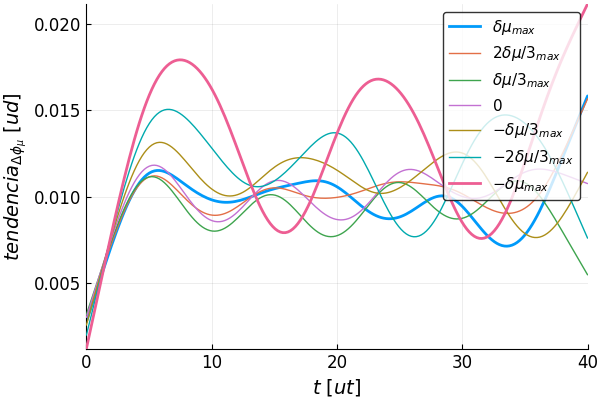
\includegraphics[width = \textwidth]{trends_tl}
\end{subfigure}
%
\begin{subfigure}{0.49\textwidth}
	\centering
	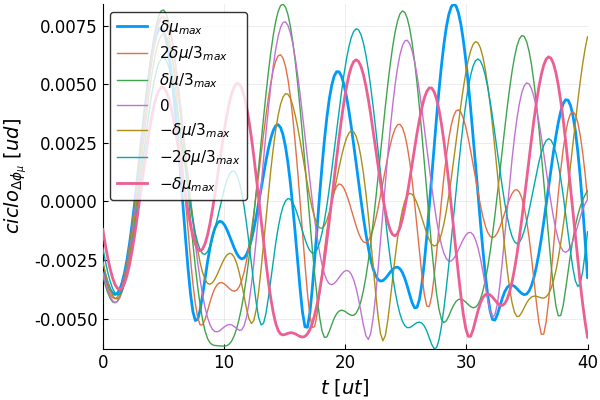
\includegraphics[width = \textwidth]{cycles_tl}
\end{subfigure}
\caption{ Separación en tendencia (izquierda) y ciclo(derecha) de los valores de la figura \ref{fig:remoteness_tl} usando un filtro de Hodrick-Prescott con $\lambda = 8000$.}
\label{fig:trendcycle_tl}
\end{figure}

\pagebreak
\section{Colisión de asteroides}
\label{sec:asteroids}

Sean $a_1$ y $a_2$ dos asteroides con la misma energía de Jacobi alrededor de la Tierra. Estos se verán afectados únicamente por la atracción gravitacional de la Tierra y la Luna. Cabe mencionar que éste es un sistema poco realista ya que, en general, habría que considerar la presencia gravitacional del Sol, la radiación solar, la geometría de los asteroides y demás efectos que influyen en la dinámica de $a_1$ y $a_2$. Por esto, esta sección plantea un modelo ilustrativo que permite ver cómo el TJ  ayuda en este tipo de situaciones. 

Inicialmente, los asteroides se encuentran a $\mathbf{x}_{a_1}(t_0) + \delta\mathbf{x}_{a_1}(t_0)$  y $\mathbf{x}_{a_2}(t_0) + \delta\mathbf{x}_{a_2}(t_0)$, respectivamente, donde $\delta\mathbf{x}_{a_i} \in \pkk{n}{2}$. La variación en cada condición representa el error de medición de éstos. Por tomar una referencia, tomemos la incertidumbre en el orden de los datos del asteroide Apophis en los años $2012 - 2028$ \cite{Desmars2013}, donde definimos $\Delta_{max} := 350 $ km como la incertidumbre máxima para los asteroides.

La figura \ref{fig:asteroid_collision_nominal_integration} muestra la trayectoria nominal de $a_1$ y $a_2$ para condiciones iniciales con energía $C_J = -1.81252 < C_J(L_1)$. En esta integración, la mínima distancia entre ambos cuerpos es de $0.00348$ que representa unos $1341$ kilómetros. Sin embargo, aunque para esta condición particular los asteroides no chocan, es posible que sí lo hagan dentro de una incertidumbre de radio $\Delta_{max}$. Esto se puede hacer con el transporte de jets de la siguiente manera: 

%FIGURA!
\begin{figure}
 \centering
 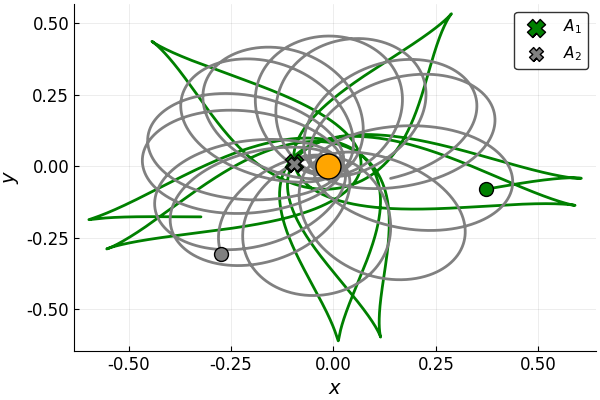
\includegraphics[width=0.7\linewidth]{asteroid_collision_nominal_integration}
 \caption{Integración nominal a $T=10 \approx $ unidades temporales, donde $\mathbf{q}_{a_1}(t_0) = \left( -0.373098, -0.0804321, 1.21995, \dot{y}_{a_1} \left( x_{a_1}(t_0), y_{a_1}(t_0), \dot{x}_{a_1}(t_0), C_J \right) \right)$ 
 y $\mathbf{q}_{a_2}(t_0) = \left( -0.27324, -0.307896, -0.307576, \dot{y}_{a_2} \left( x_{a_2}(t_0), y_{a_2}(t_0), \dot{x}_{a_2}(t_0), C_J \right) \right)$. El círculo naranja representa a $M_1$, y los círculos verde y gris a $\mathbf{q}_{a_1}(t_0)$ y $\mathbf{q}_{a_2}(t_0)$, respectivamente. La zona de mayor acercamiento se marca con cruces, donde en ésta, la distancia entre los asteroides es de $0.00348 \approx 1341$ km.}
 \label{fig:asteroid_collision_nominal_integration}
\end{figure}

\begin{itemize}
 \item Hacer una integración nominal de dos asteroides con energías similares o que se sepa que pueden tener riesgo de colisión.
 
 \item Obtener las coordenadas $\mathbf{q}_{a_i}^{(col)}$ donde la distancia entre $a_1$ y $a_2$ es mínima.
 
 \item Hacer TJ alrededor de las condiciones encontrada en el punto anterior para encontrar la parametrización de la vecindad que pasa por la zona de posible colisión.
 
 \item Encontrar la trayectoria de una distribución de $N$ puntos al evaluar los polinomios en la bola $\delta\mathbf{x}_i \leq \Delta_{max}$ alrededor de $\mathbf{q}_{a_i}^{(col)}$ para ambos asteroides y determinar la distancia entre cada par de puntos.
 
 \item Definir una distancia $D_{col}$ para la cual los asteroides chocarían y determinar qué puntos de la distribución son menores que ésta.
 
 \item Determinar la probabilidad de impacto $\mathcal{P}$ como la cantidad de veces puntos que quedan debajo de $D_{col}$ respecto al número de trayectorias totales $N^2$; así
 \begin{equation} 
 \mathcal{P} = \frac{ \# \left( \norm{\mathbf{x}_{a_1} - \mathbf{x}_{a_2} }    \leq D_{col} \right) }{N^2}.
 \end{equation}
\end{itemize}

%FIGURA!
\begin{figure}
 \centering
 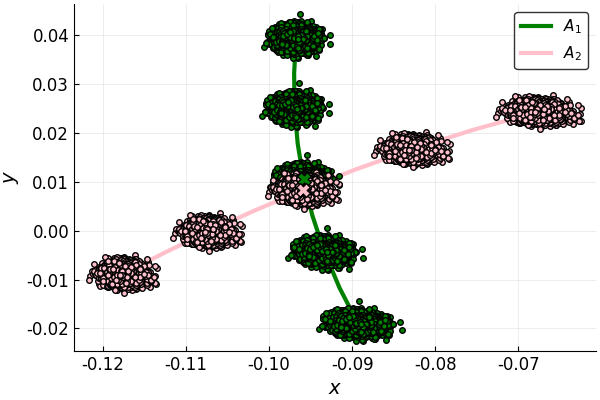
\includegraphics[width=0.7\linewidth]{asteroid_collision_distribution}
 \caption{Transporte de jets de orden $4$ alrededor de $\mathbf{q}_{a_i}^{(col)}$ (cruces en la figura) donde los cúmulos son la distribución de radio $\delta\mathbf{x}_{a_i} \leq 350$ km evaluados en el polinomio resultante del transporte. Para el método sólo se toman los cúmulos donde se encuentra $\mathbf{q}_{a_i}^{(col)}$, pero la figura busca ilustrar una sección de la trayectoria de los asteroides.}
 \label{fig:asteroid_collision_distribution}
\end{figure}

La figura \ref{fig:asteroid_collision_distribution} muestra una distribución normal de $7000$ puntos\footnote{$ N = 7000$ ya converge a una probabilidad cuyas cifras significativas no afectan el redondeo de la tabla \ref{table:collision_table}.} evaluados en el transporte alrededor de $\mathbf{q}_{a_i}^{(col)}$ para $i = \{1,2\}$. La probabilidad de impacto dependerá del tamaño que tengan los asteroides, la cual se presenta en la tabla \ref{table:collision_table}. Se presenta en la figura \ref{fig:asteroid_collision_histogram} la distribución de distancias entre ambos asteroides en la zona de riesgo de colisión. Aún cuando $D_{col}$ e incluso $\Delta_{max}$ quedan debajo del escenario más posible en la distribución, la probabilidad de impacto es suficientemente grande para no ser ignorada en los asteroides de mayor dimensión.

%TABLA!
\begin{table}[h!]
\centering
\begin{tabular}{c|c|c}
\toprule
\textbf{$ D_{col}$ [ km ]} & \textbf{$\mathcal{P}$ [ $\%$ ]} & \textbf{Colisiones [ $ \# $ ]} \\ \cmidrule(l){1-3} 
\textbf{$0.5$} &   $3.7 \times 10^{-5}$   & $18$          \\
\textbf{$5$}   &   $0.0048$               & $2356$        \\
\textbf{$30$}  &   $0.172$                & $84,609$     \\
\textbf{$150$} &   $4.357$                & $2,135,173$   \\ \bottomrule 
\end{tabular}
\caption{Número de colisiones y riesgo de choque para asteroides de distintas dimensiones.}
\label{table:collision_table}
\end{table}

%FIGURA!
\begin{figure}
 \centering
 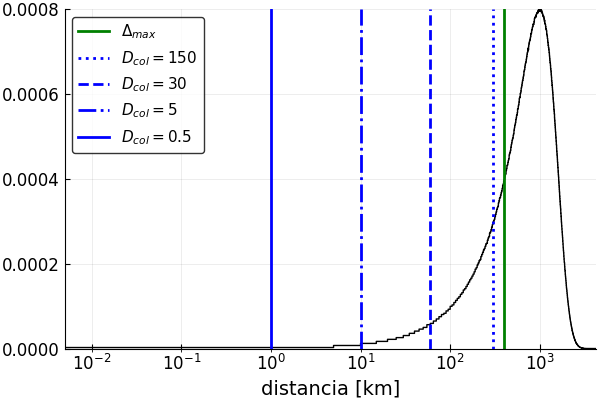
\includegraphics[width=0.7\linewidth]{asteroid_collision_histogram}
 \caption{Distribución normalizada de distancias entre $a_1$ y $a_2$ cerca del punto de posible dadas $7000$ variaciones iniciales alrededor de $\mathbf{q}_{a_1}^{col}$ y $\mathbf{q}_{a_2}^{col}$. Las líneas verticales muestran los valores usados en la tabla \ref{table:collision_table}.}
 \label{fig:asteroid_collision_histogram}
\end{figure}


Algo relevante al hacer transporte de jets es la presición de éste. Se encuentra que $\xi_{max}(\phi_{a_1}) = 0.0022 \approx 865 \ km \gg \Delta_{max}$\footnote{$\xi_{max}(\phi_{a_2})$ es prácticamente igual a $\xi_{max}(\phi_{a_1})$.}, por lo que se tiene bastante confianza en la precisión de las evaluaciones de la distribución. De hecho, al tomar una serie de variaciones $\norm{\delta\mathbf{x}_{a_i}} = \Delta_{max}$ y hacer la integración nominal de éstas, se encuentra que el error promedio respecto a éstas es del orden de $10^{-11} \approx 4 mm$, o sea, nada. Esto se muestra en la figura \ref{fig:asteroid_jt_vs_nominal}.

%FIGURA!
\begin{figure}
 \centering
 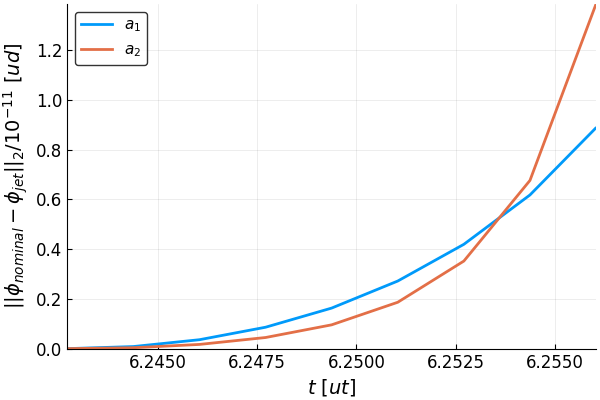
\includegraphics[width=0.7\linewidth]{asteroid_jt_vs_nominal}
 \caption{Promedio de la distancia entre la integración nominal y el transporte de jets para $500$ condiciones iniciales con variación $\norm{\delta\mathbf{x}_{a_1}} = \norm{\delta\mathbf{x}_{a_1}} = \Delta_{max}$.}
 \label{fig:asteroid_jt_vs_nominal}
\end{figure}

Así, ilustramos el método de posible colisión entre asteroides, donde se estableció la probabilidad de impacto para diferentes zonas de colisión. El transporte de jets permitió encontrar dichas probabilidades ya que en éste, simplemente hubo que evaluar la distribución de variaciones iniciales en un radio dado. Éste método es generalizable a cualquier sistema donde exista alguna incertidumbre en las condiciones iniciales. Sin embargo, hay que tener claro que el transporte de jets no es muy preciso para integraciones muy largas ni para vecindades muy grandes. En este ejemplo, el radio de las variaciones eran $0.46$ veces más pequeñas que $\xi_{max}$. Además, se hizo la integración de jets cerca del punto de posible colisión para tener tiempo de integración cortos. 

%Mencionar adimensionalización del tiempo para ver cuánto implica 1 unidad temporal.

\section{Simplecticidad del PC3C}
\label{sec:C3BP_simplecticity}

Se construyeron en el capítulo \ref{chap:CR3BP} los potenciales (\ref{eq:3body_potential}) y sus respectivas energías cinéticas (\ref{eq:3body_kinetic}) del problema general de tres cuerpos. Éstas nos permiten definir al hamiltoniano
\begin{equation}
 H(\mathbf{r}_1, \mathbf{r}_2, \mathbf{r}_3, \mathbf{p}_1, \mathbf{p}_2, \mathbf{p}_3) = \sum_{i=1}^3 h_i(r_{i,j}, r_{i,k}, \mathbf{p}_i),
 \label{eq:3BP_hamiltonian}
\end{equation} 
donde $\mathbf{p}_i = M_i \dot{\mathbf{r}}_i$ es el momento conjugado y
\begin{equation}
 h_i(r_{i,j}, r_{i,k}, \mathbf{p}_i) = \frac{1}{2 M_i} p_i^2 + U_{M_i}(r_{i,j}, r_{i,k}),
 \label{eq:individual_hamiltonian}
\end{equation}
los hamiltonianos para cada una de los cuerpos. Notemos que (\ref{eq:3BP_hamiltonian}) no depende del tiempo y, por lo tanto, es un sistema conservativo. 

Cuando en la sección \ref{sec:R3BP} se supuso que la masa menor no influye en la dinámica de las masas primarias, bastó con hacer una rotación con velocidad angular $\Omega$ para encontrar las ecuaciones de movimiento de $m_3$. Esto fija las masas primarias, cancela sus hamiltonianos ($  U_{M_2} = - U_{M_1}$) y define al hamiltoniano para la masa menor. Dicha rotación se puede realizar bajo el cambio de coordenadas
\begin{align*}
 x &= X\cos (\Omega t) - Y \sin (\Omega t), \\
 y &= X\sin (\Omega t) - Y \cos (\Omega t), 
\end{align*} 
con $(x,y)$ y $(X,Y)$ las nuevas y viejas coordenadas para $m_3$, respectivamente, tal como se muestra en la figura \ref{fig:FIGURA!}.

%FIGURA!

Para obtener el hamiltoniano modificado, que en alguna literatura se llama kamiltoniano \cite{Goldstein2007, Johns2011}, es necesario ver cómo se modifica el momento conjugado en el nuevo sistema donde, para esto, se debe conservar el principio de mínima acción

\begin{align}
 \delta \int_{t_0}^t \left( \dot{\mathbf{R}} \cdot \mathbf{P} - H(\mathbf{R}, \mathbf{P}, \tau) \right) d\tau &= 0 \nonumber \\
\implies \delta \int_{t_0}^t \left( \dot{\mathbf{r}} \cdot \mathbf{p} - K(\mathbf{r}, \mathbf{p}, \tau) \right) d\tau &= 0
 \label{eq:kamiltonian_condition}
\end{align}
en ambos ejes, lo cual sucede si
\begin{equation}
 \dot{\mathbf{R}} \cdot \mathbf{P} - H(\mathbf{R}, \mathbf{P}) = \dot{\mathbf{r}} \cdot \mathbf{p} - K(\mathbf{r}, \mathbf{p}, t) + \frac{dG(\mathbf{R}, \mathbf{p}, t)}{dt}.
\end{equation}
Aquí $\mathbf{P} = (P_x,P_y)$, $\mathbf{R} = (X,Y)$, $\mathbf{p} = (p_x,p_y)$, $\mathbf{r} = (x,y)$, $K$ es el kamiltoniano y $G = - \mathbf{r} \cdot \mathbf{p} + G_2(\mathbf{R}, \mathbf{p}, t)$ es una función que genera una transformación canónica entre ambos sistemas, también conocida como función generatriz de tipo 2 \cite{CanonicalTransformations}. Notemos que como 
\begin{align*}
 \frac{dG}{dt} =  - \dot{\mathbf{r}}\cdot \mathbf{p} - \mathbf{r}\cdot \dot{\mathbf{p}} + \pder{G_2}{\mathbf{R}}\dot{\mathbf{R}} + \pder{G_2}{\mathbf{p}}\dot{\mathbf{p}} + \pder{G_2}{t},
\end{align*}
entonces
\begin{align}
 \mathbf{P} &= \pder{G_2}{\mathbf{R}} \nonumber, \\
 \mathbf{r} &= \pder{G_2}{\mathbf{p}} \nonumber, \\
 \therefore K(\mathbf{r}, \mathbf{p}) &= H(\mathbf{r}, \mathbf{p}) + \pder{G_2}{t} (\mathbf{r}, \mathbf{p}).
 \label{eq:kamiltonian_formulae}
\end{align}

Definimos $G_2$ simplemente como
\begin{equation}
 G_2(\mathbf{R}, \mathbf{p}, t) = p_x \underbrace{\left( X \cos (\Omega t) - Y \sin (\Omega t) \right) }_{x} + p_x (\underbrace{ \left( X \sin (\Omega t) + Y \cos (\Omega t) \right)}_{y}
 \label{eq:generating_function}
\end{equation}

y, con (\ref{eq:kamiltonian_formulae}), permite formular explícitamente al kamiltoniano como
\begin{equation*}
 K(\mathbf{r}, \mathbf{p}) = \underbrace{ \frac{1}{2M_3}\left( p_x^2 + p_y^2 \right) - G \frac{M_1}{r_{1,3}} - G \frac{M_2}{r_{2,3}}}_{H(\mathbf{r}, \mathbf{p}) } + \underbrace{\Omega\left( p_y x - p_x y \right) }_{\pder{G}{t}(\mathbf{r}, \mathbf{p})}
\end{equation*}

\begin{equation}
 \therefore K = \frac{1}{2M_3} \left( (p_x - \Omega y)^2 + (p_y + \Omega x)^2 \right) - \left(G \frac{M_1}{r_{1,3}} + G \frac{M_2}{r_{2,3}} + \frac{\Omega^2}{2}\left( x^2 + y^2 \right) \right).
 \label{eq:kamiltonian}
\end{equation}

Notemos que $K = k_3$, así que la partícula menor define al hamiltoniano del sistema en el nuevo sistema de referencia. Esta nos permite probar numéricamente la propiedad simpléctica del PC3C que, contruido de otro modo, no hubiese sido evidente. Basta con hacer las transformaciones 
\begin{align}
p_x &\to p_x - \Omega y, \\
p_y &\to p_y + \Omega x,
\label{eq:momentum_transformation}
\end{align} 
y aplicar la relación (\ref{eq:sympletic_flow}).

%FIGURA!
\begin{figure}[h!]
\centering
\begin{subfigure}{0.49\textwidth}
	\centering
	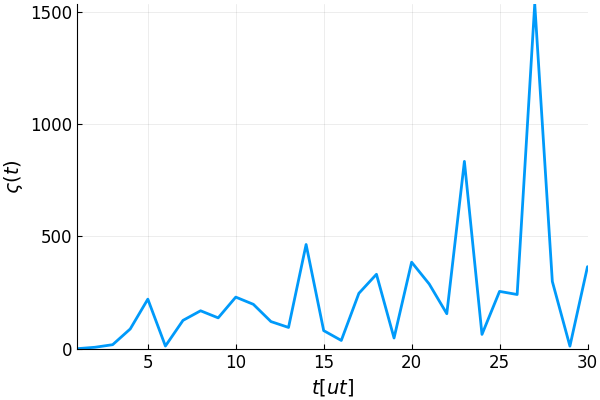
\includegraphics[width = \textwidth]{non_symplectic_L1}
\end{subfigure}
%
\begin{subfigure}{0.49\textwidth}
	\centering
	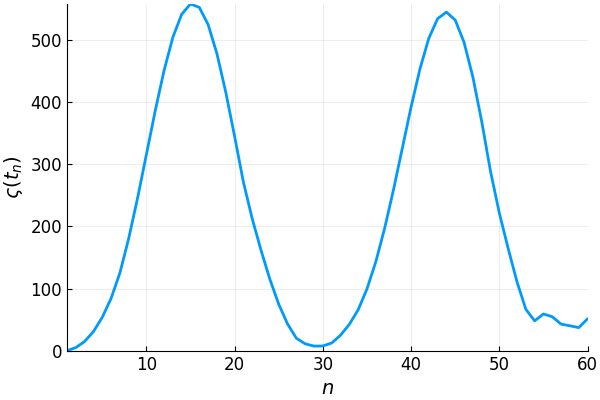
\includegraphics[width = \textwidth]{non_symplectic_L4}
\end{subfigure}
\caption{ $\varsigma(t)$ para $\phi(t)$ sin modificar el flujo en unidades adimensionales del PC3C. Las condiciones iniciales son $\xo = \left( \left( L_{1_x}, 0.001, 0, 0 \right)^T + \delta \xi \right) $ (izquierda) y $ \xo = \left( \left( L_{4_x}, L_{4_y} + 0.001, 0, 0 \right)^T + \delta \xi \right) $ (derecha) para $\delta \xi$ un polinomio de orden $3$.}
\label{fig:non_symplectic_L4_L1}
\end{figure}

Si uno no hace dichas transformaciones, parecerá que el problema no conserva la forma simpléctica, tal como en el ingenuo intento que se muestra en la figura \ref{fig:non_symplectic_L4_L1} para diferentes condiciones iniciales. Para obtener $\varsigma$ se utiliza la ecuación (\ref{eq:scalar_symplecticity}) que, como se discute en la sección \ref{sec:formas-simplecticas}, opera de manera muy natural con el TJ, ya que la parametrización de vecindades del espacio fase permite computar al jacobiano en cada punto de manera directa.

La figura \ref{fig:symplectic_L4_L1}, en cambio, muestra la conservación simpléctica del PC3C bajo la transformación (\ref{eq:momentum_transformation}), donde se observa cómo $\varsigma(t)$ se mantiene constante durante toda la integración. En ésta, se tomaron las mismas dos condiciones iniciales que en la figura \ref{fig:non_symplectic_L4_L1}; una cerca de $L_4$, que es una trayectoría estable, y otra cerca de $L_1$, que orbita alrededor de la masa primaria menor. Se puede observar cómo en la condición más estable la conservación de la simplecticidad varía en unos dos órdenes de magnitud menos que cerca de $L_1$. Sin emabrgo, ambas tienen variaciones menor a $10^{-10}$ en cada punto de la trayectoria, por lo que podemos decir que, en efecto, el sistema es simpléctico. Esta es una aplicación muy directa para el TJ que aprovecha su estructura paramétrica, de la cual se pueden obetener el jacobiano o incluso variaciones de órdenes mayores. 

%FIGURA!
\begin{figure}[h!]
\centering
\begin{subfigure}{0.49\textwidth}
	\centering
	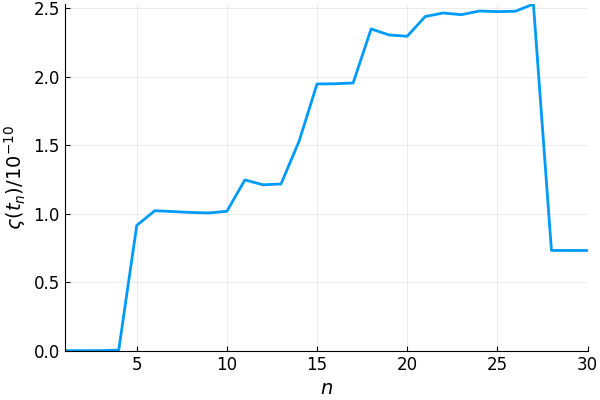
\includegraphics[width = \textwidth]{symplectic_L1}
\end{subfigure}
%
\begin{subfigure}{0.49\textwidth}
	\centering
	\includegraphics[width = \textwidth]{symplectic_L4}
\end{subfigure}
\caption{$\varsigma(t)$ para $\phi(t)$ con las transformaciones (\ref{eq:momentum_transformation}). Las condiciones iniciales son $\xo = \left( \left( L_{1_x}, 0.001, 0, 0 \right)^T + \delta \xi \right) $ (izquierda) y $ \xo = \left( \left( L_{4_x}, L_{4_y} + 0.001, 0, 0 \right)^T + \delta \xi \right) $ (derecha) para $\delta \xi$ un polinomio de orden $3$.}
\label{fig:symplectic_L4_L1}
\end{figure}

%Valdrá la pena hacer un análisis simpléctico de mayor dimensión?

\section{Campos de $\xi_{max}$ y $\varsigma_\pm$ para el PC3C}
\label{sec:C3BP_heatmaps}

El estudio y exploración del TJ ha utilizado la ecuación (\ref{eq:ximax}) en varias ocaciones. Ésta ha sido el parámetro que nos ha permitido saber qué tan grandes pueden ser las vecindades dado cierto error $\epsilon_{jet}$, tal como se discute en la sección \ref{sec:ximax}. Éste se utilizó en la sección \ref{sec:asteroids} para comprobar que la incertidumbre de medición diera resultados precisos al evaluar la distribución de puntos, y en \ref{sec:parametrization} para las variaciones del parámetro de masa y analizar la estabilidad de $L_4$. $\xi_{max}$ percibe, en esencia, qué tan compleja es la deformación de la vecindad y qué tanto se alejan las condiciones vecinas a la condición nominal, por lo que $\xi_{max} \ll 1$ implica una alta sensibilidad en las condiciones iniciales cercanas o un gran gradiente de velocidades para la vecindad. 

Para esta sección se hará un análisis del PC3C de los campos escalares de $\xi_{max}$ así como las tasas de expansión y contracción discutidas en \ref{sec:contraccion_expansion}. Dichos campos son comparables con el campo de ELTF desarrollado al principio del capítulo \ref{chap:jt_indicators}, por lo que se hará una comparación con estos al final de la sección. En el problema restringido el gradiente apunta siempre hacia las masas primarias del sistema, lo cual se puede observar en la figura \ref{fig:C3BP_ximax1}, donde se calcula el campo escalar para $\xi_{max}$ a $T = 0.3$ unidades adimensionales. Ésta es semejante a la representación de curvas de nivel de la figura \ref{fig:3body_pseudo_potential} de la sección \ref{sec:lag_points} y, al tener un tiempo de integración muy corto, no da tiempo a una gran deformación de las vecindades, planteando únicamente los lugares de mayor gradiente de velocidad. En todas las figuras que se presentan se ignoraron los puntos muy cercanos a las masas primarias, ya que el tiempo de computo es muy grande cerca de estos. 

%FIGURA! 
\begin{figure}
 \centering
 \includegraphics[width=0.8\linewidth]{C3BP_ximax1}
 \caption{Campo escalar de los tamaños máximos de vecindad $\xi_{max}$ en una retícula de $70 \times 70$  después de $0.3$ unidades adimensionales de tiempo. Éste se calculó con tolerancia $\epsilon_{Taylor} = 10^{-7}$, orden de jets $ = 2$ y orden máximo de la expansión $M = 20$. Las condiciones del PC3C son para $\xo = (x_{0_i}, y_{0_j}, 0, 0)^T$ con $\mu = 0.1$}
 \label{fig:C3BP_ximax1}
\end{figure}

La figura \ref{fig:C3BP_ximax3}, en cambio, presenta el mismo campo escalar pero integrada a $T = 3$ unidades adimensionales. Como se menciona al inicio de esta sección, las dos principales formas en las que $\xi_{max}$ sea chica es si el gradiente de velocidades en una vecindad es muy grande o si la deformación de la vecindad inicial es muy pronunciada. ambas figuras se observa cómo $\xi_{max}$ decrece gradualmente al aumentar el gradiente de velocidad hacia las singularidades. Esto muestra la tendencia de la tercer partícula atrayéndose hacia las masas primarias. Sin embargo, en la figura \ref{fig:C3BP_ximax3} se observan curvas donde $\xi_{max}$ es pequeña  respecto a los valores vecinos. Los puntos en estas curvas, a las cuales llamaremos $\mathcal{C}_s$, no reflejan un gran gradiente de velocidad, pero sí una deformación muy pronunciada del jet. Aquí seguramente divirgieron las condiciones por debajo y por arriba de la condición inicial. 

%FIGURA! 
\begin{figure}
 \centering
 \includegraphics[width=0.8\linewidth]{C3BP_ximax3}
 \caption{Mismas condiciones que para la figura \ref{fig:C3BP_ximax1} pero integrado a $3$ unidades temporales.}
 \label{fig:C3BP_ximax3}
\end{figure}

Para reforzar este análisis, se computaron las direcciones de mayor expansión para la vecindad de los puntos lagrangianos. La figura \ref{fig:C3BP_seprate3} presenta dichas direcciones en distintas secciones del espacio de configuraciones, donde se observa cómo en las zonas de menor expansión, equivalentes a las zonas donde $\xi_{max}$ es pequeña,  $\theta_{+}$ cambia drásticamente. Esto nos hace entender a las curvas como una especie de separatriz del problema. Esta figura presenta una acercamiento alrededor de $L_4$ y $L_3$, donde se observa cómo la dirección de  $\theta_{+}$ cambia cuando se cruza por una curva $\mathcal{C}_s$. Lejos de las singularidades el gradiente tiende hacia ellas pero al cruzar por estas curvas especiales, la dirección de expansión máxima cambia de sentido. 


%FIGURE!
\begin{figure}
 \centering
 \includegraphics[width=1.0\linewidth]{C3BP_seprate}
 \caption{Campos vectoriales dados por $\left( \cos(\theta_{+}(\xo), \sin(\theta_{+}(\xo) \right)^T$ sobre los campos escalares $\varsigma_{+}(\xo)$ en una cuadrícula de $20 \times 20$, con tolerancia $\epsilon_{Taylor} = 10^{-20}$, orden de los jets $M=2$ y orden de la expansió-n de Taylor $N = 25$ integradas a $T = 3$ unidades adimensionales. Las condiciones del PC3C son para $\xo = (x_{0_i}, y_{0_j}, 0, 0)^T$ con $\mu = 0.1$. A la izquierda se observan los puntos cerca de $L_4$, marcada con $\times$, mientras que a la izquierda se presentan las localidades de $L_3$.}
 \label{fig:C3BP_seprate3}
\end{figure}

Notemos de la figura \ref{fig:C3BP_FTLE}, que el campo escalar para $\xi_{max}$ es bastante similar al campo de los ELTF. Se presentan las mismas líneas separatrices que en \ref{fig:C3BP_ximax3}. Sin embargo, la diferencia conceptual es que en el caso de ELTF éstas representan las zonas de mayor tasa de expansión, mientras que en $\xi_{max}$ representan el tamaño donde las variaciones son más pequeñas.

%FIGURE!
\begin{figure}
 \centering
 \includegraphics[width=0.7\linewidth]{C3BP_FTLE}
 \caption{Campo escalar dado por los ELTF. Las condiciones y la retícula para esta figura son idénticas a las de \ref{fig:C3BP_ximax3}.}
 \label{fig:C3BP_FTLE}
\end{figure}

%Un poquito más de choro ya con la imagen, procurar ser más preciso en los datos dados y compararlo con algunas otras cosas... que no sea todo tan cualitativo, pues. Usar, potencialmente las CV0.

%Hacer una mejor discusión sobre estas órbitas, ver las energías de Jacobi y ver si, en efecto, éstas corresponden a los mismo lugares.
%Análisis de energía de las separatrices, ver si éstas tienen la misma  +- epsilon. 

%Ver si funciona ximax para el espacio planteado por Perez en su artículo, así hay punto de comparación. hacer referencia a las estructuras lagrangianas que se encuentran... si se encuentran.

%FIGURA! 

%Cerrar el capítulo de resultados con un bonito choro... 



% Para que de nuevo haya salto de linea. (buscar Dutch style)
\setlength{\parskip}{1.3ex plus 0.2ex minus 0.2ex}

\chapter{Conclusiones} 
\label{chap:conclusions}
\documentclass[letterpaper,12pt]{book}
\usepackage[spanish]{babel}
\decimalpoint 
\usepackage[utf8]{inputenc}

\usepackage{mathrsfs}
\usepackage{amsmath}
\usepackage{amssymb}
\usepackage{amsfonts}

\begin{document}



\end{document}

 
% Para que de nuevo haya salto de linea. (buscar Dutch style)
\setlength{\parskip}{1.3ex plus 0.2ex minus 0.2ex}


 
%%%%%%%%%%%%%%%%%   APÉNDICES   %%%%%%%%%%%%%%%%%
\cleardoublepage 
\phantomsection  %para el anclado este en la pagina correcta
\addcontentsline{toc}{chapter}{Apéndices}
\chaptermark{Apéndices} %cambia el encabezado
\appendix

% Reajuste de los encabezados para que diga Apendice 
\pagestyle{fancy}
\fancyhead[LO]{\leftmark}
\fancyhead[RE]{\emph{Apéndice \thechapter}}
\renewcommand{\headrulewidth}{0.5pt}

\chapter{El código}
\label{chap:code}
\input{Chapters/codigo}

\chapter{Mecánica Analítica}
\label{chap:mecanics}
Una buena forma de explorar cómo evoluciona un sistema dinámico que describa a un ente físico es encontrando las ecuaciones de movimiento que lo representa. Éste es el enfoque principal de la mecánica analítica de Hamilton y Lagrange\footnote{Claramente no son los únicos que desarrollaron esta teoría; grandes como Euler, Poisson o Liouville hicieron grandes aportaciones a la mecánica analítica, sin embargo, Hamilton y Lagrange cargan la bandera de la teoría gracias a que desarrollaron las ecuaciones de movimiento que llevan su nombre.} que, inspirados por Newton, encuentran la mejor descripción de sistemas macroscópicos basados en marcos de referencia inerciales\footnote{La elección de marcos de referencia inerciales dejan de lado la descripción relativista del mundo para esta teoría.}. Siempre que se hable de un sistema mecánico nos estaremos limitando a estas constricciones.

Un sistema mecánico está descrito a partir de las partículas que se mueven en él y de la interacción entre ellas. Una \textit{partícula} es un cuerpo puntual\footnote{Aquí es donde el concepto de macroscópico toma sentido; un cuerpo es macroscópico si se puede ver como un conjunto de objetos puntuales o partículas. En la mecánica cuántica, por ejemplo, esto no es así.}, es decir, el tamaño y dimensiones de ésta son despreciados y sólamente importará para su descripción la \textit{cantidad de materia y/o carga} que ocupa, su \textit{posición} respecto a un marco de referencia y su \textit{velocidad} en un instante dado. Un cuerpo macroscópico, como un balón de fútbol, puede describirse como un conjunto de partículas que interaccionan entre sí y cómo interaccionan éstas con el mundo externo que es, a su vez, otro conjunto de partículas. Dichas interacciones definen la energía que pueden intercambiar estas partículas y generalmente se le conoce como el \textit{potencial}. El movimiento intrínseco de éstas también conlleva cierta energía que dependerá de la cantidad de materia y la velocidad de éstas; a dicha energía se le refiere usualmente como \textit{cinética}.

Tomando como referencia un sistema de coordenadas cartesiano, podemos definir la posición de una partícula con su radio-vector $\mathbf{r}$ y su velocidad $\mathbf{v}$, que definimos como $\mathbf{v} := \frac{d \mathbf{r}}{dt} := \dot{\mathbf{r}}$. En general, una partícula vive en un espacio tridimensional así que necesita de tres coordenadas para describir su posición; un sistema de N partículas necesitará 3N coordenadas para describir la posición de todas. Resulta ser que si se conocen todas las posiciones y velocidades del sistema en un instante dado, se puede calcular, en principio, la dinámica de todo el sistema desde ese instante en adelante.\footnote{También se puede saber la dinámica desde ese instante hacia atrás; esa discusión se tendrá un poco más adelante.}

%FIGURA!


Dada la naturaleza del sistema, a veces es posible describir un sistema de N partículas con menos de 3N coordenadas. Ejemplo de esto se ilustra en la figura \ref{fig:circular_scheme}, donde la posición de una partícula $m$ se puede determinar con precisión si se conoce el radio $R$ respecto al centro del círculo, en el cual $m$ se mueve en relación a $\theta$, el ángulo respecto a alguna línea de referencia que creamos conveniente. Para este ejemplo, basta únicamente de $\theta$ para describir la trayectoria de $m$ en lugar de las 3 coordenadas que se mencionaban en el párrafo anterior; podemos pensar que dicha partícula está \textit{restringida} a moverse sobre el círculo de radio $R$, es decir, ésta pierde la libertad de moverse arbitrariamente en cualquier punto del espacio tridimensional en donde vive. Con esto, definimos como \textit{grados de libertad} al número mínimo de coordenadas independientes con las cuales se puede definir la posición de todas las partículas de un sistema.

\subsection{Principio de Mínima Acción}
\label{sec:least_action}

Un sistema tiene, en general, $s \leq N$ grados de libertad. Esto significa que se puede describir con $s$ cantidades independientes $\lbrace q_1, \ldots, q_s \rbrace$ que definen completamente la posición de todas las partículas. A estas cantidades se le llaman las \textit{coordenadas generalizadas} del sistema, y asociadas a ellas están las \textit{velocidades generalizadas} $\dot{q_i} = \frac{dq_i}{dt} \  \forall \ i \in [1,s]$. Parece ser que a la naturaleza\footnote{al menos a este nivel} le gusta seguir los caminos en los que la \textit{acción} sea mínima. Es decir, si a un instante $t_1$ el sistema ocupa las posiciones $q^{(1)} := (q_1(t_1), \ldots, q_s(t_1))$ y al instante $t_2$ las posiciones $q^{(2)}$,  debe existir una función $L$ con unidades de energía que dependa de las cantidades $q$, $\dot{q}$ y el tiempo tal que la integral
\begin{equation}
 S = \int_{t_1}^{t_2} L(q,\dot{q},t) dt
 \label{eq:action}
\end{equation}
sea mínima.\footnote{Notemos que $S$ tiene unidades de acción: $[ S ] = [energía \times tiempo]$.} Esta condición se conoce como el \textit{principio de mínima acción} o de \textit{principio de Hamilton}. A $L$ se le conoce como el \textit{lagrangiano} del sistema.

Supongamos que $q = q(t)$ es la trayectoria que minimiza a \ref{eq:action}, entonces cualquier variación $\delta q(t)$ a $q(t)$ hace que $S$ incremente. Tomaremos, sin pérdida de generalidad, el caso $s = 1$. Obviamente, $\delta q(t_1) = \delta q(t_2) = 0$ ya que, aunque queremos que la trayectoria tome un camino alternativo, éste debe empezar y terminar en los mismos puntos que $q(t)$.

Con esto, la variación en $S$ será
\begin{align*}
 \delta S = \int_{t_1}^{t_2} \delta L dt = \int_{t_1}^{t_2} \left( \pder{L}{q} \delta q + \pder{L}{ \dot{q} } \delta \dot{q} + \cancelto{0}{\mathcal{O}(\delta q^2)} \right) dt
\end{align*}

donde buscamos $\delta S = 0$ para que $S$ sea mínimo. Observando que $\delta \dot{q} = \delta \frac{dq}{dt}$ e integrando por partes, tenemos que

\begin{align*}
 \delta S &= \int_{t_1}^{t_2} \pder{L}{q} \delta q dt + \pder{L}{\dot{q}} \cancelto{0}{\delta q} \rvert_{t_1}^{t_2} - \int_{t_1}^{t_2} \frac{d}{dt} \left( \pder{L}{\dot{q}} \right) \delta q dt\\
 &= \int_{t_1}^{t_2} \left( \pder{L}{q} - \frac{d}{dt} \left( \pder{L}{ \dot{q} } \right) \delta q dt \right) = 0.
\end{align*}

Así, imponiendo la condición de que el integrando sea idénticamente cero, obtenemos las \textit{ecuaciones de movimiento de Lagrange}
\begin{equation}
 \pder{L}{d q_i} - \frac{d}{dt} \left( \pder{L}{ \dot{q_i} } \right) = 0 \ \forall \ i \in [1, \ldots, s],
 \label{eq:lagrange_equations}
\end{equation}

que son $s$ ecuaciones diferenciales ordinarias de segundo orden y, por tanto, $2s$ constantes o condiciones iniciales $\{ q_{1_0}, \ldots, q_{s_0}, \dot{q_{1_0}}, \ldots, \dot{q_{s_0}} \}$\footnote{Se entiende que $q_{i_0} = q_i(t_0)$.} son necesarias para resolverlas. Con esto, la pregunta primordial es: ¿Qué forma tiene $L$?

\subsection{Lagrangiano de la partícula libre}

Tomemos como primer caso a la partícula libre (de interacciones). Ésta no tiene constricciones ni interactúa con nadie más y, por tanto, tiene 3 grados de libertad. Tomaremos como marco de referencia inercial las coordenadas rectangulares definidas por $\{ \hat{\imath}, \hat{\jmath}, \hat{k} \}$ al cual llamaremos $\mathcal{K}$. Es importante para la descripción notar que en un marco de referencia inercial el espacio es homogéneo e isotrópico y el tiempo homogéneo.

Así, por la homogeneidad del éstos, $L$ no puede depender explícitamente de $\mathbf{r}$ ni de $t$ y, por tanto, $L(\mathbf{r},\mathbf{v},t) = L(\mathbf{v})$. Además, por lo isotrópico del espacio, debería ser indistinto para $L$ la dirección en la que la partícula se esté moviendo, de modo que la dependencia deberá sobre la magnitud de la velocidad, i.e., $L = L(\mathbf{v}) = L(v^2)$.

Por (\ref{eq:lagrange_equations}), tenemos que
 \begin{align*}
 \pder{L(\mathbf{v}) }{ \mathbf{r} } = 0 &\implies \frac{d}{dt}\pder{L(\mathbf{v})}{\mathbf{v}} = \frac{d}{dt} \frac{dL(\mathbf{v})}{d\mathbf{v}} = 0 \\
 &\therefore \mathbf{v} = \text{constante}.
 \end{align*}


Hay que resaltar dos detalles sobre el lagrangiano para continuar con esta descripción:
\begin{enumerate}

  \item Dos lagrangianos $L$ y $\mathcal{L}$ que difieren bajo una función $f(q,t)$ de la forma $\mathcal{L}(q,\dot{q},t) = L(q,\dot{q},t) + \frac{d f(q,t)}{dt}$ son equivalentes ya que $\delta S_{L} = \delta S_{\mathcal{L}} = 0$\footnote{$ \delta S_{\mathcal{L}} = \cancelto{0}{\delta S_L} + \delta f(q^{(2)},t_2) - \delta f(q^{(1)},t_1) = \pder{f(q^{(2)},t_2)}{q} \cancelto{0}{ \delta q^{(2)} } - \pder{f(q^{(1)},t_1)}{q} \cancelto{0}{ \delta q^{(1)} } = 0$.} y, por tanto, la forma de las ecuaciones definidas por (\ref{eq:lagrange_equations}) no cambia.

 \item Si dos lagrangianos $L_1$ y $L_2$ no interactúan entre sí en un mismo sistema, entonces ambos se pueden englobar en uno mismo como la suma indivudual de sus partes, i.e.
 \begin{equation}
  L = L_1 + L_2 .
  \label{eq:lagrangian_addititivy}
 \end{equation}

\end{enumerate}

Por lo primero, podemos encontrar la forma explícita de $L$ para la partícula libre. Sabemos que en el marco $\mathcal{K}$ la partícula se mueve con velocidad $\mathbf{v}$. Si otro marco inercial $\mathcal{K}'$ se mueve a $\mathbf{\epsilon} \ll \mathbf{v}$ respecto a $\mathcal{K}$, entonces la partícula se con velocidad $\mathbf{v}' = \mathbf{v} + \mathbf{\epsilon}$ en $\mathcal{K}'$. Así,
\begin{align*}
 \mathcal{L} = L(v'^2) = L(v^2 + 2 \mathbf{v} \cdot \mathbf{\epsilon} + \epsilon^2) \\
 \implies  L(v'^2) = L(v^2) + \pder{L}{v^2} 2 \mathbf{v} \cdot \mathbf{\epsilon} + \cancelto{0}{\mathcal{O}(\epsilon^2)}.
\end{align*}
Como $\mathcal{L}$ y $L$ sólo pueden diferir por la derivada temporal de alguna función $f(\mathbf{v},t)$, entonces
\begin{align*}
 \pder{L}{v^2} = \alpha
\end{align*}
y, por tanto
\begin{equation}
 L(v^2) = \alpha v^2 = \frac{1}{2}m v^2,
\end{equation}
con $m$ la masa de la partícula, consiguiendo que el lagrangiano tenga unidades de energía.

Por lo segundo, como las partículas libres, por definición, no interactúan entre sí, el lagrangiano de un sistema de $N$ partículas libres será
\begin{equation}
 L(\mathbf{v}_1, \ldots, \mathbf{v}_N) = L_1(\mathbf{v}_1) + \ldots + L_N(\mathbf{v}_N) = \sum_{i=1}^N \frac{1}{2}m_i v_i^2.
 \label{eq:kinetic}
\end{equation}

Notemos que este particular lagrangiano describe la energía del movimiento de las partículas cuando no interaccionan entre ellas; por esto, en el panorama más general, se le conoce como la \textit{energía cinética} del sistema: $L_{libre}(\mathbf{v}) := T(\mathbf{v})$.

\subsection{Lagrangiano de un sistema cerrado}

Un sistema de N partículas se llama cerrado si éstas interaccionan únicamente entre ellas; es decir, no hay agentes externos que alteren al sistema. Vimos que la energía cinética está dada por (\ref{eq:kinetic}) y, así, al lagrangiano se le debe agregar la interacción entre partículas o \textit{energía potencial}. Resulta que si el sistema es cerrado, el potencial será una función que depende únicamente de la posición que cada partícula tiene en un instante dado. Nombraremos $-U$ a esta función, y así
\begin{equation}
 L(\mathbf{r},\mathbf{v}) = \sum_{i=1}^N \frac{1}{2}m_i v_i^2 -U(\mathbf{r_1},\ldots,\mathbf{r_N}).
 \label{eq:lagrangian_cartesian_closed}
\end{equation}

Hay tres puntos que creo vale la pena mencionar. Primero, Como $U$ es función de las posiciones únicamente entonces, si la posición de cualquier partícula cambia, el potencial  afecta instantaneamente a todas las demás. Segundo, si suponiéramos que dichas interacciones no son instantáneas, entonces éstas se propagarían con cierta velocidad y, por tanto, la invarianza de las ecuaciones sobre marcos de referencia inerciales ya no sería válida. Tercero, sustituyendo (\ref{eq:lagrangian_cartesian_closed}) en (\ref{eq:lagrange_equations}) tenemos
\begin{align}
 -\pder{U(\mathbf{r_1}, \ldots, \mathbf{r_N})}{\mathbf{r}_i} &= \frac{d}{dt} \pder{}{\mathbf{v}_i} \sum_{i=1}^N \frac{1}{2}m_i v_i^2 \nonumber \\
 &\therefore m_i \ddot{\mathbf{r}_i} = -\pder{U(\mathbf{r_1}, \ldots, \mathbf{r_N})}{\mathbf{r}_i} =: \mathbf{F}_i(\mathbf{r}) \nonumber \\
 &\therefore \mathbf{F}(\mathbf{r}) = \sum \mathbf{F}_i(\mathbf{r}) = - \nabla U(\mathbf{r}),
 \label{eq:newton_second_law}
\end{align}
que corresponde a la \textit{segunda ley de Newton} para sistemas cerrados; de ahí la elección del ``$-$'' para la función $U$.

Ahora, el lagrangiano dado por (\ref{eq:lagrangian_cartesian_closed}) fue trabajado en coordenadas rectangulares dado que la partícula libre no tiene constricciones del espacio. Como el potencial puede que restringa las trayectorias en el que las partículas se mueven, es posible que el sistema pueda ser descrito en $s < 3N$  coordenadas generalizadas en donde existe una función $\mathbf{g}_j: \mathbb{R}^{s} \to \mathbb{R}^{N}, \ j \in \{1,2,3\}$ tal que $g_{j,i}(q) = x_{j,i}$, donde $\mathbf{r}_i = x_{1,i} \hat{\imath} + x_{2,i} \hat{\jmath} + x_{3,i} \hat{k}$, $\dot{x}_{j,i} = \sum_k \pder{\mathbf{g}_j(q)}{q_k} \dot{q_k}$ y $q \in \mathbb{R}^s$. Metiendo todo esto en el lagrangiano obtenemos
\begin{equation}
 L(q,\dot{q}) = \frac{1}{2}\sum_{i,k} a_{i,k}(q) \dot{q_i}\dot{q_k} - U(q),
 \label{eq:lagrangian_closed_generalized}
\end{equation}

el lagrangiano en coordenadas generalizadas, donde $\mathbf{a}(q)$ es la función que sale de sustituir la transformación en $T(\dot{\mathbf{r}}) = \frac{1}{2}\sum m_i \left( \dot{x}_{1,i}^2 + \dot{x}_{2,i}^2 + \dot{x}_{3,i}^2 \right)$. Es interesante destacar que en coordenadas generalizadas la energía cinética puede depender de las posiciones generalizadas y es, como antes, cuadrática en las velocidades.

\subsection{Lagrangiano de un sistema abierto}

Un sistema abierto es aquel que puede interactuar con sus alrededores. Si un sistema $A$ interactúa con un sistema $B$ decimos, desde la perspectiva de $A$, que éste se mueve en un campo externo dado por $B$. Suponiendo que el sistema conformado por $A$ y $B$ juntos es cerrado, entonces tendrá un lagrangiano
\begin{equation}
 L(q_A,q_B,\dot{q}_A,\dot{q}_B) = T_A(q_A,\dot{q}_A) + T_B(q_B,\dot{q}_B) - U(q_A,q_B),
\end{equation}
con $U$ un potencial que considera la interacción de todas las partículas $q_A$ y $q_B$.

Como no nos interesa la treyectoria de las partículas de $B$ sino únicamente en cómo afecta a $A$, podemos sustituir  en el lagrangiano $q_B \to q_b(t)$, la solución explicita en $t$ para $B$, obteniendo
\begin{align*}
 L(q_A,\dot{q}_A,t) = T_A(q_A,\dot{q_A}) + \cancelto{\frac{df}{dt}}{T_B(t)} - U(q_A,q_B(t)).
\end{align*}

Así, un sistema que interactúa con un campo externo difiere con uno cerrado sólo en el potencial, que tendrá una dependencia explícita del tiempo
\begin{equation}
 L(q,\dot{q},t) = T(q,\dot{q}) - U(q,t).
 \label{eq:lagrangian_open_generalized}
\end{equation}

\subsection{Marcos de referencia no inerciales}
\label{sec:ficticious_forces}

Se ha hablado hasta aquí de sistemas descritos por marcos de referencia inerciales. Dicha necesidad emerge de la invarianza ante estos y de la invarianza, así, de las ecuaciones de movimiento. Sin embargo, hay sistemas donde resulta más cómoda la descripción si el marco de referencia tiene ciérta aceleración respecto a los marcos de referencia inerciales con los que hemos trabajado. Un auto que busca tomar una curva en una carretera desde el punto de vista del piloto o un satélite que navega las órbitas entre dos planetas desde el punto del satélite son dos buenos ejemplos de esto. La aceleración dada por el marco de referencia brindará, según la segunda ley de Newton ($\ddot{\mathbf{r}}_{ref} \neq 0$), una fuerza extra al sistema siempre que un móvil masivo interactúe con él. A este tipo de fuerzas se le llaman \textit{ficticias}, ya que no son provocadas por campos externos ni interacción entre partículas, únicamente por la elección de un sistema de referencia que no va a velocidad constante.

Veremos como ejemplo las fuerzas ficticias que aparecen en un marco de referencia en rotación respecto a uno inercial. Ésto ilustará cómo trabajar en marcos de referencia no inerciales y se usará posteriormente para el problema de los tres cuerpos.

\subsubsection{Marcos rotantes}

Sea un marco que rota respecto algún eje de simetría con velocidad angular $\theta(t)$. Si basamos un marco de rerefencia inercial tal que el eje de rotación coincida con el eje $z$, entonces como se muestra en la figura \ref{fig:}, la relación entre ambos se puede expresar en coordenadas cilíndricas como
\begin{align}
 \hat{\imath}_r(t) &= \cos \theta(t) \hat{\imath}_i + \sin \theta(t) \hat{\jmath}_i \nonumber \\
 \hat{\jmath}_r(t) &= -\sin \theta(t) \hat{\imath}_i + \cos \theta(t) \hat{\jmath}_i \\
 \hat{k}_r(t) &= \hat{k}_i \nonumber
 \label{eq:rotating_unitaries}
\end{align}
donde los subíndices ``$r$'' y ``$i$'' se refieren a los marcos de referencia rotado e inercial, respectivamente. Así, el cambio de los unitarios respecto al tiempo son
\begin{align}
 \frac{d}{dt} \hat{\imath}_r(t) &= \dot{\theta}(t) \left( -\sin \theta(t) \hat{\imath}_i + \cos \theta(t) \hat{\jmath}_i  \right) \nonumber \\
 \frac{d}{dt} \hat{\jmath}_r(t) &= \dot{\theta}(t) \left( -\cos \theta(t) \hat{\imath}_i - \sin \theta(t) \hat{\jmath}_i \right) \\
 \frac{d}{dt} \hat{k}_r &= 0 \nonumber
 \label{eq:rotating_unitaries_derivs}
\end{align}
Siguiendo la construcción de \cite{wiki_rotating_frame}, definimos al vector de rotación $\mathbf{\Omega} := \left( 0, 0, \dot{\theta} \right)$ y, con éste, cualquier término de (\ref{eq:rotating_unitaries_derivs}) se puede expresar como
\begin{equation}
 \frac{d}{dt}\hat{u} = \mathbf{\Omega} \times \hat{u}.
\end{equation}

Sea entonces $\mathbf{f}(t) = f_x(t) \hat{\imath} + f_y(t) \hat{j} + f_z(t) \hat{k}$ una cantidad definida en el marco que rota, la descripción de su derivada desde el marco de referencia inercial es, por la regla del producto,
\begin{equation*}
 \left( \frac{d \mathbf{f}}{dt} \right)_i = \left( \frac{d\mathbf{f}}{dt} \right)_r  + \mathbf{\Omega} \times \mathbf{f}
\end{equation*}
y, por tanto,
\begin{equation}
 \left(\frac{d}{dt}\right)_i := \left( \frac{d}{dt} \right)_r + \mathbf{\Omega} \times
 \label{eq:rotating_derivative}
\end{equation}
es un operador que expresa la derivada de $\mathbf{f}$ en el marco de referencia inercial.

Con (\ref{eq:rotating_derivative}) se pueden expresar la velocidad
\begin{equation}
 \mathbf{v}_i = \dot{\mathbf{r}}_i = \mathbf{v}_r + \mathbf{\Omega} \times \mathbf{r}_r,
 \label{eq:rotating_velocity}
\end{equation}
y la aceleración
\begin{align}
 \mathbf{a}_i = \ddot{\mathbf{r}}_i &= \left[ \left( \frac{d}{dt}\right)_r + \mathbf{\Omega} \times \right]\left[ \mathbf{v}_r + \mathbf{\Omega} \times \mathbf{r}_r \right] \nonumber \\
 \nonumber \\
 \therefore \ddot{\mathbf{r}}_i &= \ddot{\mathbf{r}}_r + 2\mathbf{\Omega} \times \mathbf{\dot{r}}_r + \mathbf{\Omega} \times \left( \mathbf{\Omega} \times \mathbf{r}_r \right) + \dot{\mathbf{\Omega}} \times \mathbf{r}_r
 \label{eq:rotating_acceleration}
\end{align}
en relación al marco de referencia inercial del sistema.

Con esto, podemos ver que si una partícula de masa $m$ tiene una aceleración $\ddot{\mathbf{r}}$ en el marco en rotación, ésta sentirá una serie de fuerzas ficticias si es vista desde un marco inercial. Al término ``$2 m \mathbf{\Omega} \times \dot{\mathbf{r}}$'' se le conoce como \textit{fuerza centrípeta}, a ``$m \mathbf{\Omega} \times ( \mathbf{\Omega} \times \mathbf{r} )$'' como la \textit{fuerza de Coriolis} y a ``$m \dot{\mathbf{\Omega}} \times \mathbf{r}$'' como \textit{fuerza de Euler}.

Notemos que si la rotación es uniforme entonces $\dot{\mathbf{\Omega}} = 0$. Además, si el sistema es cerrado en el marco rotativo, entonces, por (\ref{eq:newton_second_law}), (\ref{eq:rotating_acceleration}) se reduce a
\begin{equation}
 \ddot{\mathbf{r}}_r + 2\mathbf{\Omega} \times \dot{\mathbf{r}}_r = \ddot{\mathbf{r}}_i - \nabla \left( \frac{1}{m}U(\mathbf{r}_r) +  \frac{1}{2} \mathbf{\Omega}^2 \mathbf{r}_r^2 \right).
 \label{eq:rotating_constant_acceleration}
\end{equation}

Salvo por la fuerza de Coriolis, que vuelve a éste un sistema abierto, se tiene que las ecuaciones de movimiento expresan un sistema cerrado con el nuevo potencial $U_{tot}(\mathbf{r}) = U(\mathbf{r}_r) + \frac{m}{2} \mathbf{\Omega}^2 \mathbf{r}_r^2$.\footnote{Si $\Omega = (0,0,\text{constante})$, entonces $\mathbf{\Omega} \times ( \mathbf{\Omega} \times \mathbf{r} ) =\Omega^2 r_r = \nabla \frac{1}{2}\Omega^2 r_r^2$.}

%Revisar ésto bien en sintaxis y signos y ver qué nos interesa en cada caso entre "i" y "r".
%Meter imágenes.

\subsection{Ecuaciones de Hámilton}
\label{sec:hamilton}

Estableciendo el principio de mínima acción encontramos qué condiciones debe satisfacer el lagrangiano. Ésta condición define las ecuaciones de movimiento del sistema en cuestión en términos de las posiciones, las velocidades y el tiempo $q, \dot{q}$ y $t$, respectivamente. Sin embargo, nada dice que éstas sean las únicas cantidades para describir a dicho sistema. En la formulación de las ecuaciones de movimiento de Hámilton, un sistema es descrito por $q,p$ y $t$, las posiciones generalizadas, el momento generalizado y el tiempo, respectivamente. De manera similar a lagrangiano, que es una función $L = L(q,\dot{q},t)$, llamaremos \textit{hamiltoniano} a la función que represente las ecuaciones de movimiento equivalentes, donde $H = H(q,p,t)$. Resulta conveniente muchas veces trabajar en este esquema ya que el hanmiltoniano representa a la energía total mecánica de este. Se puede pasar de un esquema al otro vía una transformada de Legandre.

Sabemos que
\begin{equation}
 dL = \sum_i \pder{L}{q_i} d q_i + \sum_i \pder{L}{\dot{q_i} }  d\dot{q_i}
 \label{eq:lagrangian_differential}
\end{equation}
y, definiendo
\begin{equation}
 p_i := \pder{L}{\dot{q}_i}
\end{equation}
obtenemos, sustituyendo en (\ref{eq:lagrange_equations}) que
\begin{equation}
 \pder{L}{q_i} = \dot{p}_i.
 \label{eq:dot_momentum}
\end{equation}

Por otro lado, por la regla del producto, observamos que $d\left( \sum p_i \dot{q}_i \right) = \sum p_i d \dot{q}_i + \sum d p_i \dot{q}_i$. Usando esto, y mezclándolo con (\ref{eq:dot_momentum}) y (\ref{eq:lagrangian_differential}), obtenemos
\begin{align}
 dL &= \sum_i \dot{p}_i d q_i + \sum_i p_i d \dot{q}_i \nonumber \\
 \implies d\left(\sum_i p_i \dot{q}_i - L \right) &= - \sum_i \dot{p}_i d q_i + \sum_i \dot{q}_i d p_i.
 \label{eq:legandre_ham_lag}
\end{align}

Como $H = H(q,p,t)$, entonces
\begin{equation}
 dH = \sum_i \pder{H}{q_i} dq_i + \sum_i \pder{H}{dp_i} dp_i,
 \label{eq:hamilton_differential}
\end{equation}
y, comparándolo con (\ref{eq:legandre_ham_leg}), concluimos que el hamiltoniano está dado por
\begin{equation}
 H = \sum_i p_i \dot{q}_i - L
 \label{eq:hamiltonian_legandre}
\end{equation}
y define las ecuaciones de movimiento
\begin{align}
 &\pder{H}{q_i} = - \dot{p}_i && \pder{H}{p_i} = \dot{q}_i.
\end{align}

Como el hamiltoniano representa la energía total del sistema, nos puede interesar cómo cambia en una trayectoria dada; así
\begin{equation*}
 \frac{dH}{dt} = \pder{H}{t} + \sum_i \pder{H}{p_i}\dot{p}_i + \sum_i \pder{H}{q_i}\dot{q}_i = \pder{H}{t} + \sum_i - \cancel{\dot{p}_i\dot{q}_i} + \cancel{\dot{p}_i\dot{q}_i} = \pder{H}{t}.
\end{equation*}
Observamos que si $H$ no depende explícitamente del tiempo entonces es constante, i.e.,
\begin{equation*}
 H(p,q) = \text{constante} \ \forall (q,p) \in q(t).
\end{equation*} Esto no es más que la conservación de la energía mecánica para un sistema cerrado.\footnote{Equivalentemente al lagrangiano, si el hamiltoniano no depende explícitamente del tiempo será un sistema cerrado; si sí, entonces será abierto.}

Otro punto interesante sobre la descripción hamiltoniana es que $H$ puede expresarse de una manera más elegante notando que la energía cinética es cuadrática en las velocidades, entonces
\begin{align*}
 \sum_i \dot{q}_i \pder{L}{\dot{q_i}} = \sum_i \dot{q}_i \pder{T}{\dot{q_i}} = 2 T.
\end{align*}
Sustituyendo esto último en (\ref{eq:hamiltonian_legandre}) obtenemos
\begin{align}
 H = 2T - L = 2T - \left( T - U \right) \nonumber \\
 \nonumber \\
 \therefore H(q,p,t) = T(q,p) + U(q,t).
 \label{eq:hamiltonian}
\end{align}
El hamiltoniano de un sistema es la suma de las energías cinética y potencial de éste.
  

\backmatter %los capitulos y titulos de nivel inferior no aparecen numerados

 
\pagestyle{plain} %Reajuste en encabezados
%\cleardoublepage %supuestamente necesario si tuviera mas de una pagina
\phantomsection  %para el anclado este en la pagina correcta
\addcontentsline{toc}{chapter}{Bibliografía}
\chaptermark{Bibliografía} %cambia el encabezado


\bibliographystyle{ieeetr}    

%\setlength{\bibsep}{4pt}
%\begin{spacing}{0.9} 
\bibliography{Chapters/biblio}
%\end{spacing}


       
\end{document}     